\documentclass[12pt,a4paper]{article}
\usepackage[utf8]{inputenc}
\usepackage[T1]{fontenc}
\usepackage[french]{babel}
\usepackage{geometry}
\usepackage{enumitem}
\usepackage{xcolor}
\usepackage{setspace}
\usepackage{titlesec}
\usepackage{hyperref}
\usepackage{natbib}
\usepackage{csquotes}
\usepackage{booktabs}
\usepackage{multirow}
\usepackage{colortbl}
\usepackage{graphicx}
\usepackage{float}
\usepackage{caption}
\usepackage{amsmath}
\usepackage{amssymb}
\usepackage{parskip}
\usepackage{tikz}
\usetikzlibrary{arrows.meta, positioning, calc, fit}

% --- Professional Color Palette ---
\definecolor{primary}{RGB}{33, 150, 243}
\definecolor{secondary}{RGB}{75, 75, 75}
\definecolor{accent}{RGB}{0, 150, 136}
\geometry{margin=2.5cm, top=2.5cm, bottom=2.5cm}
\setlength{\parindent}{0pt}
\onehalfspacing

% --- Section title formatting ---
\titleformat{\section}{\large\bfseries}{}{0em}{}[\titlerule]
\titleformat{\subsection}{\normalsize\bfseries}{}{0em}{}
\titleformat{\subsubsection}{\normalsize\itshape}{}{0em}{}

% --- Hyperref setup ---
\hypersetup{colorlinks=true, linkcolor=blue, citecolor=black, urlcolor=blue}

% --- Bibliography style ---
\bibliographystyle{apalike}

\begin{document}

% ======================================================
% TITLE PAGE
% ======================================================
\begin{titlepage}
\begin{center}

% ---- Header ----
\begin{minipage}{0.18\textwidth}
\raggedright

\includegraphics[height=2.7cm]{logos/logofsjeste.png}
\end{minipage}
\hfill
\begin{minipage}{0.78\textwidth}
\raggedleft
{\small Royaume du Maroc}\\[2pt]
{\large Universit\'e Abdelmalek Essa\^adi}\\[2pt]
{\normalsize Facult\'e des Sciences Juridiques, \'Economiques et Sociales}\\
{\normalsize T\'etouan}
\end{minipage}

\vspace{0.8cm}

% ---- Memoire ----
{\normalsize \textsc{M\'emoire de Fin d'\'Etudes}}\\[4pt]
{\small Pour l'obtention du Master en}\\[2pt]
{\normalsize \textbf{Finance, Actuariat et Data Science}}

\vspace{0.3cm}
\rule{\textwidth}{0.5pt}
\vspace{0.4cm}

% ---- TITLE ----
{\large \textbf{L'APPORT DE L'INTELLIGENCE ARTIFICIELLE}}\\[4pt]
{\normalsize \textbf{DANS LA PR\'EVISION BUDG\'ETAIRE}}\\[6pt]
{\small \textit{Cas du Minist\`ere de la Justice du Maroc}}

\vspace{0.4cm}
\rule{\textwidth}{0.5pt}

\vspace{0.6cm}

% ---- Author ----
\begin{flushleft}
\textbf{R\'ealis\'e par :}\\[2pt]
\hspace{0.4cm} ABBARI Fatima Ezzahraa
\end{flushleft}

\vspace{0.25cm}

% ---- Supervisors ----
\begin{flushleft}
\textbf{Encadr\'e par :}\\[2pt]
\hspace{0.4cm} Pr. DAKKON Mohamed, Professeur \`a la FSJES de T\'etouan\\
\hspace{0.4cm} M. ZABARATOU Iliass, Encadrant professionnel
\end{flushleft}

\vfill

% ---- Bottom: logo + academic year ----
\begin{center}

\includegraphics[height=2.4cm]{logos/ministry.png}\\[10pt]
\rule{0.35\textwidth}{0.4pt}\\[6pt]
{\footnotesize Ann\'ee universitaire : 2025--2026}
\end{center}

\vspace{0.2cm}

\end{center}
\end{titlepage}

% ---- TABLE OF CONTENTS ----
\pagenumbering{arabic}
\newpage
\tableofcontents
\newpage

% ======================================================
% REMERCIEMENTS
% ======================================================
\phantomsection
\section*{Remerciements}
\addcontentsline{toc}{section}{Remerciements}

\begin{center}

Au terme de ce travail, je tiens à exprimer ma sincère gratitude envers toutes les personnes qui ont contribué, de près ou de loin, à sa réalisation.

\vspace{0.4cm}

Je remercie en premier lieu \textbf{Monsieur Iliass Zabaratou}, mon encadrant professionnel, pour m'avoir guidé dans la définition du sujet de ce mémoire et pour m'avoir accordé sa confiance tout au long du stage.

\vspace{0.4cm}

Mes remerciements s'adressent également au \textbf{Professeur Mohamed Dakkon}, coordinateur du Master Finance, Actuariat et Data Science et encadrant académique de ce travail, pour son soutien, ses orientations et sa disponibilité.

% \vspace{0.4cm}

% Je souhaite exprimer ma profonde reconnaissance à \textbf{Monsieur Bilal Khanfoud}, dont l'aide a été déterminante à plusieurs étapes de ce travail.

% \vspace{0.4cm}

J'adresse mes sincères remerciements aux cadres et professionnels du bureau, et en particulier à \textbf{Zakaria} et \textbf{Kaoutar}, qui m'ont guidé dès le premier jour et ont veillé à ce que mon intégration se déroule dans les meilleures conditions. Je tiens également à exprimer ma gratitude envers \textbf{Khaoula}, \textbf{Idrissi}, \textbf{Fatima} et \textbf{Taoufiq} pour leurs conseils avisés et leur soutien constant tout au long de cette expérience.

\vspace{0.4cm}

Enfin, je remercie l'ensemble du corps enseignant du Master Finance, Actuariat et Data Science de la FSJES de Tétouan pour la qualité de la formation dispensée, ainsi que ma famille pour son soutien indéfectible.

\end{center}

\newpage

% ======================================================
% DÉDICACE
% ======================================================
\phantomsection
\section*{D\'edicace}
\addcontentsline{toc}{section}{D\'edicace}

\begin{center}
\vspace*{3cm}

\textit{\`A mes parents,}\\[4pt]
\textit{pour tout ce qu'ils ont sacrifi\'e pour que j'en arrive l\`a.}

\vspace{0.8cm}

\textit{\`A mon fr\`ere,}\\[4pt]
\textit{pour sa pr\'esence et son soutien au quotidien.}

\vspace{0.8cm}

\textit{\`A mes amis,}\\[4pt]
\textit{pour les moments partag\'es et les encouragements.}

\vspace{1.2cm}

\textit{Je d\'edie ce travail.}

\end{center}

\newpage

% ======================================================
% RÉSUMÉ
% ======================================================
\phantomsection
\section*{R\'esum\'e}
\addcontentsline{toc}{section}{R\'esum\'e}

Ce m\'emoire examine dans quelle mesure les approches de \textit{Machine Learning} peuvent am\'eliorer la pr\'ecision de la pr\'evision budg\'etaire au sein du Minist\`ere de la Justice du Maroc, par rapport aux m\'ethodes statistiques classiques.

La d\'epense publique marocaine est encadr\'ee depuis 2015 par la Loi Organique relative \`a la Loi de Finances (LOF~130-13), qui impose une budg\'etisation par la performance et une programmation triennale. Dans ce contexte, la fiabilit\'e des pr\'evisions de cr\'edits constitue un enjeu institutionnel majeur~: un \'ecart important entre pr\'evision et ex\'ecution expose le minist\`ere \`a des critiques parlementaires et \`a des observations de la Cour des Comptes.

\`A partir d'un jeu de donn\'ees trimestrielles reconstitut\'e \`a partir des morasses budg\'etaires annuelles et des rapports de la Tr\'esorerie G\'en\'erale du Royaume (2020--2025, 109~lignes budg\'etaires), nous \'evaluons quatre mod\`eles~: une moyenne historique et un d\'ecalage annuel (benchmarks), une r\'egression Lasso, et un algorithme de gradient boosting (XGBoost). La validation repose sur un protocole \textit{walk-forward} \`a fen\^etre expansive (4~folds sur 2022--2025), conforme \`a la contrainte de causalit\'e temporelle. Un module de d\'etection d'anomalies bas\'e sur le score~$z$ compl\`ete le dispositif en signalant les lignes en sous-ex\'ecution anormale en cours d'exercice.

Les r\'esultats montrent que les mod\`eles de Machine Learning, et en particulier XGBoost, offrent des gains de pr\'ecision substantiels par rapport aux benchmarks, tout en permettant une interpr\'etabilit\'e op\'erationnelle gr\^ace aux importances de variables. Ces r\'esultats sont int\'egr\'es dans un tableau de bord interactif d\'evelopp\'e en Python, mis \`a disposition de la Direction du Budget.

\bigskip
\noindent\textbf{Mots-cl\'es~:} pr\'evision budg\'etaire, Machine Learning, Lasso, XGBoost, LOF~130-13, Minist\`ere de la Justice, walk-forward, d\'etection d'anomalies.

\newpage

% ======================================================
% ABSTRACT
% ======================================================
\phantomsection
\section*{Abstract}
\addcontentsline{toc}{section}{Abstract}

This thesis investigates whether Machine Learning approaches can improve the accuracy of budget execution forecasting at the Moroccan Ministry of Justice, compared to classical statistical methods.

Moroccan public expenditure has been governed since 2015 by the Organic Finance Law (LOF~130-13), which introduced performance-based budgeting and a three-year programming framework. In this context, the reliability of budget forecasts has become a major institutional challenge: significant deviations between forecasts and actual execution expose the Ministry to parliamentary scrutiny and Court of Accounts observations.

Using a quarterly dataset reconstructed from annual budget documents (\textit{morasses budgétaires}) and Treasury General reports (2020--2025, 109 budget lines), we evaluate four models: a historical mean and an annual lag (benchmarks), a Lasso regression, and a gradient boosting algorithm (XGBoost). Validation follows a walk-forward protocol with an expanding window (4~folds over 2022--2025), strictly respecting temporal causality. A Z-score anomaly detection module complements the system by flagging budget lines with abnormal under-execution during the fiscal year.

Results show that Machine Learning models, particularly XGBoost, achieve substantial accuracy gains over the benchmarks while maintaining operational interpretability through variable importance scores. These results are integrated into an interactive Python dashboard made available to the Budget Directorate.

\bigskip
\noindent\textbf{Keywords:} budget forecasting, Machine Learning, Lasso, XGBoost, LOF~130-13, Ministry of Justice, walk-forward validation, anomaly detection.

\newpage

% ======================================================
% TABLE DES FIGURES
% ======================================================
\phantomsection
\addcontentsline{toc}{section}{Table des figures}
\listoffigures

\newpage

% ======================================================
% LISTE DES TABLEAUX
% ======================================================
\phantomsection
\addcontentsline{toc}{section}{Liste des tableaux}
\listoftables

\newpage

% ======================================================
% LISTE DES ACRONYMES
% ======================================================
\phantomsection
\section*{Liste des acronymes}
\addcontentsline{toc}{section}{Liste des acronymes}

\begin{tabular}{@{}ll@{}}
\textbf{IA}   & Intelligence Artificielle \\
\textbf{ML}   & Machine Learning \\
\textbf{LOF}  & Loi Organique relative \`a la Loi de Finances \\
\textbf{MJ}   & Minist\`ere de la Justice \\
\textbf{TGR}  & Tr\'esorerie G\'en\'erale du Royaume \\
\textbf{GID}  & Gestion Int\'egr\'ee de la D\'epense \\
\textbf{PLF}  & Projet de Loi de Finances \\
\textbf{RMSE} & Root Mean Squared Error \\
\textbf{MAE}  & Mean Absolute Error \\
\textbf{MAPE} & Mean Absolute Percentage Error \\
\end{tabular}

\newpage

% ======================================================
% INTRODUCTION GÉNÉRALE
% ======================================================
\phantomsection
\section*{Introduction g\'en\'erale}
\addcontentsline{toc}{section}{Introduction g\'en\'erale}

La pr\'evision budg\'etaire est au c\oe{}ur de la gouvernance financi\`ere publique. Pour un minist\`ere comme celui de la Justice du Maroc, anticiper avec pr\'ecision l'ex\'ecution des cr\'edits n'est pas un exercice formel~: c'est une condition de coh\'erence entre les ambitions programmatiques et les capacit\'es r\'eelles de d\'epense. Pourtant, malgr\'e les progr\`es introduits par la r\'eforme de la Loi Organique relative \`a la Loi de Finances (LOF~130-13), les \'ecarts entre pr\'evisions et r\'ealisations demeurent significatifs, notamment pour les d\'epenses d'investissement.

Face \`a ce constat, les approches de \textit{Machine Learning} offrent une piste prometteuse. En exploitant des structures non lin\'eaires, en mutualisant l'information entre lignes budg\'etaires et en s'adaptant aux donn\'ees courtes, ces m\'ethodes pourraient combler les limites des outils statistiques classiques utilis\'es jusqu'ici.

\phantomsection
\subsection*{Contexte et Probl\'ematique}
\addcontentsline{toc}{subsection}{Contexte et Probl\'ematique}

Depuis l'entr\'ee en vigueur de la LOF~130-13 en 2015 et sa mise en \oe{}uvre progressive jusqu'en 2020, le cadre budg\'etaire marocain a profond\'ement \'evolu\'e. La budg\'etisation par la performance, la programmation triennale et l'obligation de sinc\'erit\'e budg\'etaire (article~10) ont renforc\'e les exigences en mati\`ere de fiabilit\'e des pr\'evisions. Dans ce contexte, un \'ecart important entre pr\'evision et ex\'ecution expose le minist\`ere \`a des critiques parlementaires et \`a des observations de la Cour des Comptes.

Le Minist\`ere de la Justice pr\'esente par ailleurs des caract\'eristiques sp\'ecifiques qui compliquent la pr\'evision~: une masse salariale rigide repr\'esentant plus de 70\,\% des d\'epenses de fonctionnement, des d\'epenses d'investissement fortement concentr\'ees sur le dernier trimestre, et une nomenclature budg\'etaire d\'ecompos\'ee en plus d'une centaine de lignes h\'et\'erog\`enes.

C'est dans ce contexte que s'inscrit la probl\'ematique de ce m\'emoire~:

\begin{center}
\textit{Dans quelle mesure les approches de Machine Learning peuvent-elles am\'eliorer la pr\'ecision de la pr\'evision de l'ex\'ecution budg\'etaire au Minist\`ere de la Justice du Maroc, par rapport aux m\'ethodes statistiques classiques~?}
\end{center}

\phantomsection
\subsection*{Objectifs de la Recherche}
\addcontentsline{toc}{subsection}{Objectifs de la Recherche}

Ce travail poursuit quatre objectifs compl\'ementaires~:

\begin{enumerate}
    \item \textbf{Analyser} le cadre institutionnel et budg\'etaire du Minist\`ere de la Justice, afin d'identifier les facteurs qui commandent l'ex\'ecution des cr\'edits.
    \item \textbf{Construire} un jeu de donn\'ees trimestrielles fiable, reconstitut\'e \`a partir des morasses budg\'etaires annuelles et des rapports de la Tr\'esorerie G\'en\'erale du Royaume (2020--2025).
    \item \textbf{\'Evaluer} quatre mod\`eles de pr\'evision -- deux benchmarks classiques, une r\'egression Lasso et un algorithme XGBoost -- selon un protocole de validation \textit{walk-forward} rigoureux.
    \item \textbf{D\'eployer} les r\'esultats dans un tableau de bord interactif Python, op\'erationnel pour la Direction du Budget.
\end{enumerate}

\phantomsection
\subsection*{M\'ethodologie}
\addcontentsline{toc}{subsection}{M\'ethodologie}

La d\'emarche adopt\'ee articule trois composantes~:

\textbf{Une phase de contextualisation} (chapitres~1 et~2)~: description de l'institution, de son budget et du cadre juridique de la gestion budg\'etaire. Cette \'etape permet d'identifier les variables explicatives pertinentes et les contraintes propres aux donn\'ees disponibles.

\textbf{Une phase th\'eorique} (chapitre~3)~: pr\'esentation des fondements du Machine Learning appliqu\'e \`a la pr\'evision de s\'eries temporelles courtes. Sont d\'etaill\'es~: le compromis biais-variance, les mod\`eles retenus (Lasso et XGBoost), les benchmarks de r\'ef\'erence, le module de d\'etection d'anomalies par score~$z$, et le protocole de validation \textit{walk-forward} \`a fen\^etre expansive.

\textbf{Une phase empirique} (chapitre~4)~: construction du jeu de donn\'ees, entra\^inement et \'evaluation des mod\`eles, analyse des r\'esultats par indicateurs d'erreur (RMSE, MAE, MAPE).

\textbf{Une phase applicative} (chapitre~5)~: conception, d\'eveloppement et \'evaluation du syst\`eme de pilotage budg\'etaire -- tableau de bord interactif Python int\'egrant les pr\'evisions et les alertes d'anomalies, d\'eploy\'e pour la Direction du Budget.

\medskip

\textbf{Structure du m\'emoire~:} Le chapitre~1 pr\'esente le Minist\`ere de la Justice. Le chapitre~2 d\'ecrit la gestion budg\'etaire et ses contraintes. Le chapitre~3 pose les fondements th\'eoriques des mod\`eles utilis\'es. Le chapitre~4 expose la mise en \oe{}uvre empirique et les r\'esultats obtenus. Le chapitre~5 d\'etaille la conception et l'\'evaluation du syst\`eme de pilotage.

\newpage

\phantomsection
\section*{Chapitre 1 : Le Minist\`ere de la Justice}\addcontentsline{toc}{section}{Chapitre 1 : Le Minist\`ere de la Justice}

\bigskip

Tout projet d'optimisation budgétaire commence par comprendre l'institution dont on pilote les crédits. Ce chapitre retrace l'évolution du Ministère de la Justice depuis 1955, décrit ses missions, et présente son organisation. Une attention particulière est portée à la Direction du Budget~-- interlocuteur direct de cette étude.
%================================================================
\phantomsection
\subsection*{1.1 \quad Historique et missions}
\addcontentsline{toc}{subsection}{1.1 Historique et missions}
%================================================================

%----------------------------------------------------------------
\phantomsection
\subsubsection*{1.1.1 \quad \'Evolution institutionnelle}
\addcontentsline{toc}{subsubsection}{1.1.1 \'Evolution institutionnelle}
%----------------------------------------------------------------

Le minist\`ere de la Justice occupe une place singuli\`ere dans l'architecture institutionnelle marocaine. H\'eritier d'une tradition juridique plurielle (islamique, coutumi\`ere et civiliste), il a connu depuis sa cr\'eation en 1955 plusieurs mutations profondes refl\'etant l'\'evolution du cadre constitutionnel et des priorit\'es de l'\'Etat. La Constitution de 2011 constitue un tournant d\'ecisif~: en consacrant l'ind\'ependance du pouvoir judiciaire et en cr\'eant le Conseil Sup\'erieur du Pouvoir Judiciaire (CSPJ), elle a red\'efini le p\'erim\`etre d'intervention du minist\`ere, recentr\'e d\'esormais sur les missions administratives, financi\`eres et logistiques d'appui au syst\`eme judiciaire \citep{MEF2015}.

Cette \'evolution s'est accompagn\'ee d'une r\'eforme progressive du syst\`eme judiciaire, articul\'ee autour de la Charte de la R\'eforme du Syst\`eme Judiciaire adopt\'ee en 2013, dont les axes ont \'et\'e d\'eclin\'es en programmes et actions budg\'etaires conform\'ement \`a la Loi Organique relative \`a la Loi de Finances n\textsuperscript{o}~130-13.

%----------------------------------------------------------------
\phantomsection
\subsubsection*{1.1.2 \quad Missions et attributions}
\addcontentsline{toc}{subsubsection}{1.1.2 Missions et attributions}
%----------------------------------------------------------------

Les missions du minist\`ere, telles que d\'efinies par le D\'ecret n\textsuperscript{o}~2.22.400 du 18~octobre~2022 relatif aux attributions et \`a l'organisation du minist\`ere de la Justice, s'articulent autour de quatre domaines principaux~:

\begin{itemize}
    \item \textbf{La gestion administrative et financi\`ere des juridictions}~: le minist\`ere assure la gestion des ressources humaines, financi\`eres et logistiques des tribunaux de l'ensemble du territoire national. Il supervise l'organisation du travail administratif des greffes et assure la coordination entre les services judiciaires et les services d\'econcentr\'es.

    \item \textbf{La gestion du patrimoine et des infrastructures judiciaires}~: construction, r\'ehabilitation et \'equipement des palais de justice et des \'etablissements p\'enitentiaires. Cette mission mobilise une part significative des cr\'edits d'investissement du minist\`ere.

\item \textbf{La transformation numérique et la modernisation du service judiciaire}~: pilotage de la transition numérique des juridictions, déploiement de plateformes dématérialisées et intégration des technologies de l’information dans les procédures judiciaires et administratives.

\item \textbf{La gestion des ressources humaines du personnel judiciaire et administratif}~: recrutement, formation, avancement et gestion pr\'evisionnelle des effectifs du corps des magistrats, des greffiers, des administrateurs et du personnel p\'enitentiaire.
\end{itemize}

Dans le cadre de la mise en \oe{}uvre de la Charte Nationale pour la Réforme du Système Judiciaire, le ministère poursuit l’édification d’une administration judiciaire professionnelle fondée sur la déconcentration administrative et financière. Le Projet de performance du PLF~2026 structure cette réforme autour de trois axes~: la modernisation de la législation, la facilitation de l’accès à la justice et la qualification de l’administration judiciaire \citep{MJNumerique2026}. Sur le plan numérique, la vision stratégique 2025--2030 vise à placer le justiciable au c\oe{}ur de la transformation en déployant une justice numérique efficace et transparente et en mobilisant l’intelligence artificielle pour faciliter le travail de l’administration judiciaire, en partenariat avec le Programme des Nations Unies pour le développement~(PNUD). Parmi les plateformes en cours de déploiement figurent la plateforme numérique du document adoulaire (dématérialisation des actes liés au mariage, au divorce et aux successions), la plateforme de traitement des demandes de certificat de nationalité marocaine pour les Marocains résidant à l’étranger, le portail de dépôt des demandes de grâce et de libération conditionnelle, ainsi que les plateformes d’échange de données avec les établissements bancaires et les compagnies d’assurance, encadrées par une convention tripartite avec l’ACAPS et la Fédération Marocaine des Assurances~(FMA).



%================================================================
\phantomsection
\subsection*{1.2 \quad Organisation}
\addcontentsline{toc}{subsection}{1.2 Organisation}
%================================================================

Sur le plan organisationnel, le minist\`ere de la Justice s'articule autour de deux composantes~: les services centraux \'etablis \`a Rabat et les services d\'econcentr\'es r\'epartis sur l'ensemble du territoire national.

%----------------------------------------------------------------
\phantomsection
\subsubsection*{1.2.1 \quad Services centraux}
\addcontentsline{toc}{subsubsection}{1.2.1 Services centraux}
%----------------------------------------------------------------

En vertu du D\'ecret n\textsuperscript{o}~2.22.400 du 18~octobre~2022, le minist\`ere de la Justice est charg\'e de l'\'elaboration et de l'ex\'ecution de la politique du gouvernement dans le domaine de la justice, sans pr\'ejudice de l'ind\'ependance du pouvoir judiciaire. L'organisation interne des divisions et services est pr\'ecis\'ee par l'Arr\^et\'e du Ministre de la Justice n\textsuperscript{o}~1501.22 du 19~octobre~2022.

L'administration centrale regroupe, sous l'autorit\'e du ministre, un Secr\'etariat G\'en\'eral, une Inspection G\'en\'erale, huit directions th\'ematiques et un institut de formation~:

\begin{itemize}
    \item La Direction des Affaires Civiles, des Professions Juridiques et Judiciaires
    \item La Direction des Affaires Criminelles, des Gr\^aces et de la Surveillance de la D\'elinquance
    \item La Direction de la L\'egislation et des \'Etudes
    \item La Direction de la Modernisation et des Syst\`emes d'Information
    \item La Direction des Ressources Humaines
    \item La Direction du Budget (\textit{Modirriyat al-Miz\^aniyya})
    \item La Direction de la Gestion des \'Equipements et du Patrimoine
    \item La Direction de la Coop\'eration et de la Communication
    \item L'Institut National du Greffe et des Professions Juridiques et Judiciaires (INFCJ)
\end{itemize}


\begin{figure}[H]
\centering
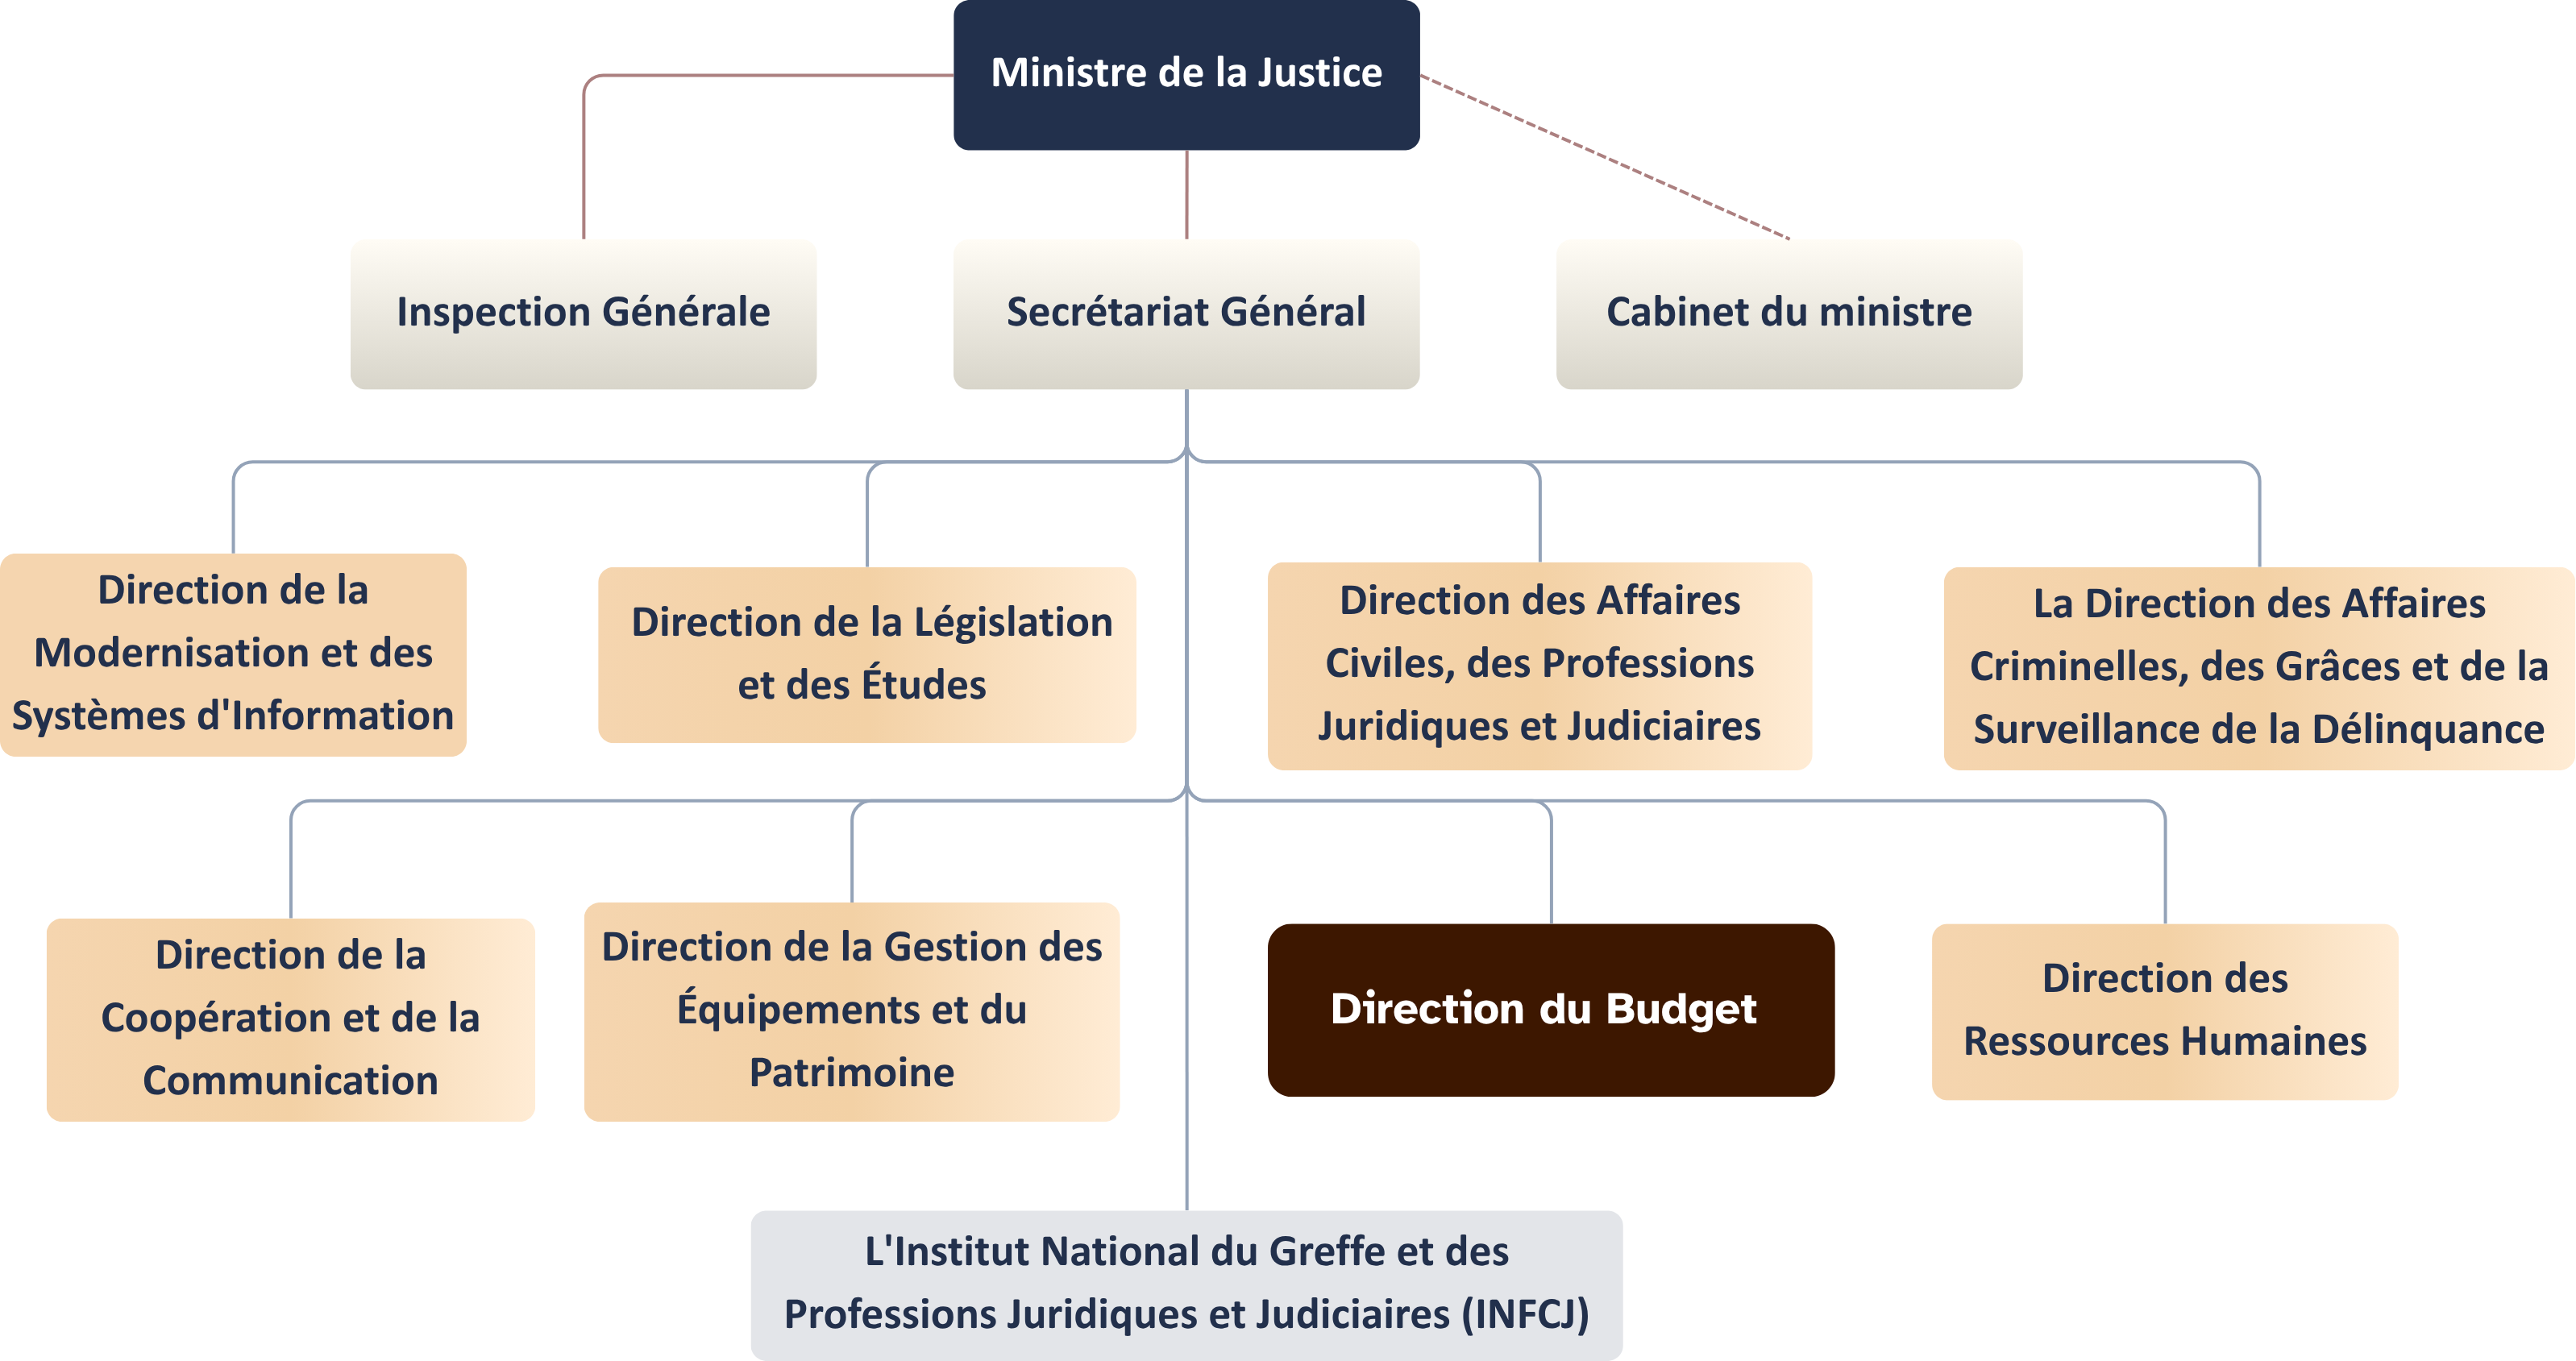
\includegraphics[width=\textwidth]{figures/organigrammeJustice.png}
\caption{Organigramme du minist\`ere de la Justice (source~: D\'ecret n\textsuperscript{o}~2.22.400).}
\label{fig:organigramme_ministere}
\end{figure}


Au sein du ministère, la Direction du Budget constitue l'interlocuteur principal avec le ministère de l'Économie et des Finances (MEF) et la Trésorerie Générale du Royaume (TGR). Son rôle est détaillé à la \hyperref[sec:direction-budget]{section~1.3}.
%----------------------------------------------------------------
\phantomsection
\subsubsection*{1.2.2 \quad Services d\'econcentr\'es}
\addcontentsline{toc}{subsubsection}{1.2.2 Services d\'econcentr\'es}
%----------------------------------------------------------------

Les services d\'econcentr\'es constituent la composante op\'erationnelle de l'institution. Ils comprennent notamment~:

\begin{itemize}
    \item La Cour de cassation (si\`ege \`a Rabat), juridiction supr\^eme de l'ordre judiciaire ordinaire
    \item Les Cours d'appel et les Cours administratives d'appel, r\'eparties dans les grandes villes du Royaume
    \item Les Tribunaux de premi\`ere instance (TPI) et les sections de justice de proximit\'e
    \item Les Tribunaux administratifs et les Tribunaux de commerce
    \item Les \'etablissements p\'enitentiaires g\'er\'es par la Direction G\'en\'erale de l'Administration P\'enitentiaire et de la R\'einsertion (DGAPR)
\end{itemize}

L'ensemble du r\'eseau judiciaire couvre les douze r\'egions du Royaume, avec des implantations dans la quasi-totalit\'e des provinces et pr\'efectures. Cette pr\'esence territoriale \'etendue explique en grande partie la complexit\'e logistique et budg\'etaire de l'institution~: des ordonnateurs secondaires d\'econcentr\'es re\c{c}oivent d\'el\'egation de cr\'edits et ex\'ecutent localement le budget, ce qui multiplie les flux budg\'etaires \`a suivre et \`a anticiper.

%================================================================
\phantomsection
\label{sec:direction-budget}
\subsection*{1.3 \quad La Direction du Budget}
\addcontentsline{toc}{subsection}{1.3 La Direction du Budget}
%================================================================

%----------------------------------------------------------------
\phantomsection
\subsubsection*{1.3.1 \quad Composition et positionnement}
\addcontentsline{toc}{subsubsection}{1.3.1 Composition et positionnement}
%----------------------------------------------------------------

Au sein de l'organigramme minist\'eriel, la Direction du Budget joue un r\^ole central dans la gestion des ressources financi\`eres de l'institution. Rattach\'ee hi\'erarchiquement au Secr\'etariat G\'en\'eral, elle constitue l'interface principale entre le minist\`ere de la Justice d'une part, et le MEF et la TGR d'autre part.

\paragraph{Composition~:}

Conform\'ement \`a l'article~30 du d\'ecret organisant les structures du minist\`ere (B.O.\ n\textsuperscript{o}~7161), la Direction du Budget comprend les entit\'es suivantes~:

\begin{itemize}
    \item \textbf{Division de la gestion du budget et de la comptabilit\'e} (\textit{qism tadbir al-miz\^aniyya wa-l-muh\^asaba})~: gestion des engagements de d\'epenses et des paiements, suivi des comptes affect\'es \`a des fins sp\'eciales, d\'el\'egations de cr\'edits aux ordonnateurs secondaires, et \'elaboration des situations annuelles d'ex\'ecution budg\'etaire.

    \item \textbf{Division des comptes des tribunaux} (\textit{qism his\^ab\^at al-mah\^akim})~: suivi et centralisation des comptes des tribunaux, gestion des comptables assign\'es aux caisses des tribunaux, et suivi des paiements \'electroniques.

    \item \textbf{Division du recouvrement} (\textit{qism al-tah\d{s}\^il})~: suivi du recouvrement des amendes et condamnations p\'ecuniaires, des frais et d\'epens judiciaires, et des paiements \'electroniques li\'es aux op\'erations de recouvrement.

    \item \textbf{Division de la pr\'evision et de la programmation financi\`ere} (\textit{qism al-tawaqqu\textquoteleft{} wa-l-barmaja al-m\^aliyya})~: \'elaboration des programmes budg\'etaires pluriannuels et du projet de budget annuel du minist\`ere, pr\'eparation du projet de performance et du rapport de nageât al-ad\^a\textquoteleft, conduite du dialogue de gestion avec les tribunaux, et pr\'evision, suivi et \'evaluation de l'ex\'ecution budg\'etaire.

    \item \textbf{Service des affaires techniques et logistiques} (\textit{masla\d{h}at al-shu\textquoteleft\^un al-tiqniyya wa-l-lujistikiyya})~: appui technique et logistique aux divisions de la direction.
\end{itemize}

C'est la \textbf{Division de la pr\'evision et de la programmation financi\`ere} qui constitue le terrain direct de notre recherche~: elle produit les pr\'evisions budg\'etaires annuelles et triennales et dispose de l'historique d'ex\'ecution n\'ecessaire \`a la mod\'elisation.

\begin{figure}[H]
\centering
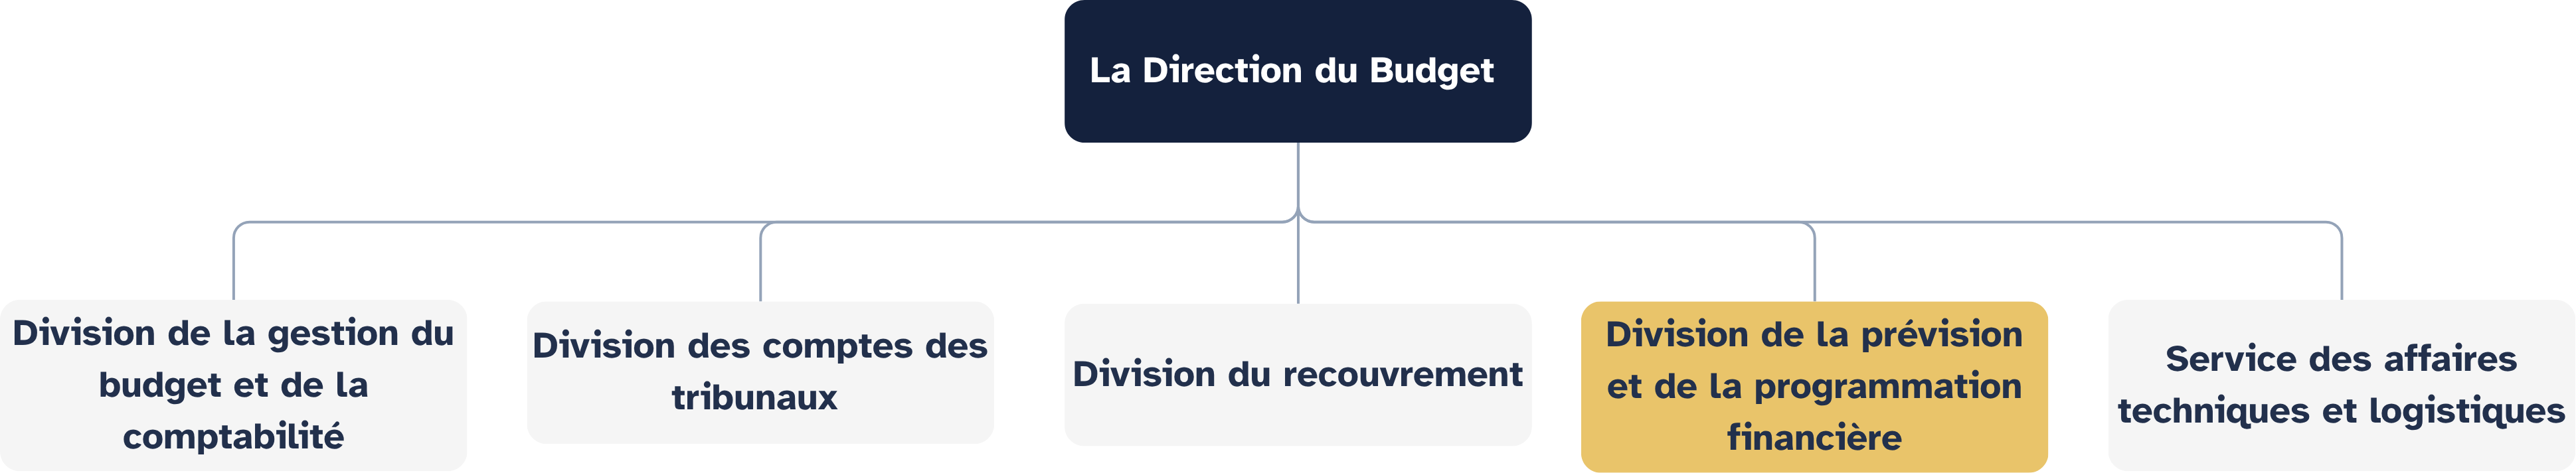
\includegraphics[width=0.95\textwidth]{figures/figure2.png}
\caption{Structure de la Direction du Budget du minist\`ere de la Justice.}
\label{fig:organigramme_db}
\end{figure}



%----------------------------------------------------------------
\phantomsection
\subsubsection*{1.3.2 \quad Fonctions et interfaces}
\addcontentsline{toc}{subsubsection}{1.3.2 Fonctions et interfaces}
%----------------------------------------------------------------

Les fonctions de la Direction du Budget couvrent l'ensemble du cycle de vie budg\'etaire~:

\begin{itemize}
    \item \textbf{La programmation budg\'etaire}~: coordination de l'\'elaboration des projets de performance annuels et triennaux (PBT-CDMT), consolidation des besoins remont\'es par les directions centrales et les services d\'econcentr\'es, et d\'efense des demandes de cr\'edits lors des conf\'erences budg\'etaires avec la Direction du Budget du MEF.

    \item \textbf{L'ex\'ecution budg\'etaire}~: gestion des cr\'edits d\'el\'egu\'es, suivi des engagements, coordination avec les ordonnateurs secondaires d\'econcentr\'es, et suivi du taux de consommation des cr\'edits en temps r\'eel via le syst\`eme GID de la TGR.

    \item \textbf{Le reporting et le contr\^ole de gestion}~: production des tableaux de bord budg\'etaires p\'eriodiques, renseignement des indicateurs de performance contractualis\'es avec le MEF, et alimentation des Rapports Annuels de Performance (RAP) transmis au Parlement conform\'ement \`a la LOF 130-13.

    \item \textbf{La gestion des archives d'ex\'ecution financi\`ere}~: extraction, compilation et archivage des \'etats d'ex\'ecution budg\'etaire mensuels produits par le syst\`eme GID, qui constituent la mati\`ere premi\`ere de notre analyse empirique (voir chapitre~3).

    \item \textbf{La gestion des restes \`a payer}~: suivi des engagements pluriannuels non encore sold\'es, coordination avec la TGR pour les ordonnancements diff\'er\'es, et pilotage de la tr\'esorerie budg\'etaire.
\end{itemize}

\paragraph{Interfaces externes~:}

Dans l'exercice de ses missions, la Direction du Budget interagit avec plusieurs acteurs ext\'erieurs au minist\`ere. La \textbf{Direction du Budget du MEF} fixe les enveloppes dans les lettres de cadrage et arbitre les demandes lors des conf\'erences budg\'etaires annuelles. La \textbf{TGR} assure l'ex\'ecution comptable et le contr\^ole des d\'epenses via le syst\`eme de Gestion Int\'egr\'ee de la D\'epense (GID), d\'eploy\'e depuis 2009 pour offrir une vision en temps r\'eel de l'\'etat de consommation des cr\'edits \citep{ElMoussali2023}. L'\textbf{Inspection G\'en\'erale des Finances (IGF)} proc\`ede \`a des audits p\'eriodiques de la gestion financi\`ere. La \textbf{Cour des Comptes} exerce le contr\^ole juridictionnel \textit{a posteriori} sur les comptes publics, et ses observations alimentent annuellement le dialogue de gestion entre le minist\`ere et le MEF.

C'est dans ce contexte que s'inscrit la probl\'ematique de ce m\'emoire. La Direction du Budget dispose d'un historique riche de donn\'ees d'ex\'ecution budg\'etaire, mais les m\'ethodes de pr\'evision conventionnelles restent insuffisamment adapt\'ees \`a la complexit\'e des dynamiques de d\'epense. Ceci soul\`eve la question centrale de notre recherche~:

\begin{center}
\textit{Dans quelle mesure les mod\'eles de Machine Learning peuvent-ils am\'eliorer
la pr\'evision du taux d'ex\'ecution budg\'etaire au sein du minist\'ere de la Justice,
et comment ces pr\'evisions peuvent-elles alimenter un syst\'eme d'aide \`a la d\'ecision
pour un pilotage proactif des cr\'edits en cours d'exercice~?}
\end{center}

Cette question ne postule pas que le Machine Learning \textit{surpasse} n\'ecessairement
les m\'ethodes statistiques classiques sur un crit\'ere de pr\'ecision brut~: elle
s'interroge sur la \textbf{valeur ajout\'ee op\'erationnelle} que ces outils peuvent
apporter \`a un gestionnaire budg\'etaire (d\'etection pr\'ecoce des lignes \`a risque,
generation de sc\'enarios, aide \`a la r\'eallocation des cr\'edits) l\`a o\'u une
simple moyenne historique ne fournit qu'une projection passive.

%----------------------------------------------------------------
\phantomsection
\subsubsection*{1.3.3 \quad La Division de Pr\'evision et de Programmation Financi\`ere}
\addcontentsline{toc}{subsubsection}{1.3.3 La Division de Prévision et de Programmation Financière}
%----------------------------------------------------------------

C'est au sein de cette direction, et plus pr\'ecis\'ement dans la \textbf{Division de Pr\'evision et de Programmation Financi\`ere} (\textit{qism al-tawaqqu\textquoteleft{} wa-l-barmaja al-m\^aliyya}), que s'est d\'eroul\'e notre stage. D\'efinie par l'article~34 du d\'ecret n\textsuperscript{o}~2.22.400\footnote{Bulletin Officiel n\textsuperscript{o}~7161 du 16~janvier~2023, page~485.}, cette division est investie des missions suivantes~:

\begin{enumerate}
    \item \textbf{\'Elaboration des programmes budg\'etaires pluriannuels et du projet de budget annexe annuel} du minist\`ere~: traduction des orientations strat\'egiques en enveloppes financi\`eres pluriannuelles (CDMT triennal) et construction du projet de budget pr\'epar\'e \`a l'occasion de chaque loi de finances.

    \item \textbf{Pr\'eparation du projet et du rapport de performance} (\textit{naja\textquoteleft{}at al-ad\^a\textquoteleft{}}) annex\'es au projet de loi de finances~: formalisation des objectifs strat\'egiques, d\'efinition des indicateurs et renseignement des cibles, conform\'ement aux exigences de la LOF~130-13.

    \item \textbf{Pr\'eparation et conduite du dialogue de gestion avec les tribunaux} (\textit{hiw\^ar al-tadbir ma\textquoteleft{}a al-mah\^akim})~: animation de la concertation annuelle avec les ordonnateurs secondaires d\'econcentr\'es pour la r\'epartition des cr\'edits et la n\'egociation des objectifs de performance.

    \item \textbf{\'Elaboration des programmes contractuels et suivi de leur ex\'ecution}~: mise en \oe{}uvre des engagements contractualis\'es avec le MEF, pilotage des programmes d'investissement pluriannuels et reporting p\'eriodique sur l'avancement physique et financier.

    \item \textbf{Pilotage financier des projets et coordination avec les partenaires institutionnels}~: gestion des partenariats, suivi des conventions de financement et articulation avec les bailleurs de fonds institutionnels.

    \item \textbf{Pr\'evision, suivi et \'evaluation de l'ex\'ecution budg\'etaire, et accompagnement des services d\'econcentr\'es} en mati\`ere financi\`ere et comptable~: c'est la mission \textit{cardinale} au regard de notre recherche. Elle implique la production de pr\'evisions de taux d'ex\'ecution \`a horizon mensuel et trimestriel, le suivi des \'ecarts entre cr\'edits ouverts et cr\'edits consomm\'es, et le conseil proactif aux ordonnateurs secondaires sur les risques de sous-ex\'ecution ou de d\'epassement.

    \item \textbf{Pr\'eparation du compte administratif et rapport sur l'ex\'ecution des d\'epenses budg\'etaires}~: cl\^oture annuelle du cycle budg\'etaire, consolidation des \'etats comptables finals et production du bilan d'ex\'ecution transmis au MEF et \`a la Cour des Comptes.
\end{enumerate}

C'est la mission~6 qui fonde directement l'utilit\'e op\'erationnelle de ce m\'emoire~: disposer de pr\'evisions d'ex\'ecution fiables et pr\'ecoces constitue, pour cette division, une exigence fonctionnelle permanente, que les m\'ethodes actuelles fond\'ees sur des extrapolations tendancielles ou des comparaisons \`a l'ann\'ee pr\'ec\'edente ne satisfont qu'imparfaitement.

%================================================================
\phantomsection
\subsection*{1.4 \quad Enjeux et objectifs du m\'emoire}
\addcontentsline{toc}{subsection}{1.4 Enjeux et objectifs du m\'emoire}
%================================================================

%----------------------------------------------------------------
\phantomsection
\subsubsection*{1.4.1 \quad Enjeux du projet}
\addcontentsline{toc}{subsubsection}{1.4.1 Enjeux du projet}
%----------------------------------------------------------------

Ce m\'emoire s'inscrit dans une d\'emarche qui d\'epasse le simple exercice acad\'emique~: il r\'epond \`a des enjeux concrets et imm\'ediats pour le minist\`ere de la Justice et, plus largement, pour la gouvernance financi\`ere publique au Maroc.

\begin{itemize}
    \item \textbf{Cr\'edibilit\'e budg\'etaire et redevabilit\'e parlementaire~:}
    La LOF~130-13 a institu\'e l'obligation pour chaque minist\`ere de produire un Rapport Annuel de Performance (RAP) pr\'esentant les r\'ealisations par rapport aux pr\'evisions. Des \'ecarts persistants entre pr\'evisions et ex\'ecution fragilisent la cr\'edibilit\'e de l'institution vis-\`a-vis du Parlement et de la Cour des Comptes~; ils signalent \'egalement un d\'eficit de pilotage interne. Le D\'ecret n\textsuperscript{o}~2-22-580 du 3~mars~2023 rend d\'esormais obligatoire, dans chaque d\'epartement minist\'eriel, un dispositif de contr\^ole de gestion destin\'e \`a \og{}v\'erifier, en permanence, l'atteinte des objectifs de performance au regard des ressources allou\'ees et \`a analyser les r\'esultats par rapport aux pr\'evisions\fg{} \citep{DecretCDG2023}. Am\'eliorer la qualit\'e pr\'edictive des pr\'evisions est donc un enjeu de gouvernance autant que de gestion.

    \item \textbf{Optimisation de l'allocation des ressources~:}
    Un minist\`ere dont les cr\'edits d'investissement sont syst\'ematiquement sous-consomm\'es en d\'ebut d'exercice et sur-sollicit\'es en fin d'ann\'ee subit un co\^ut d'opportunit\'e r\'eel~: des projets judiciaires (construction de tribunaux, \'equipement num\'erique) sont retard\'es, des restes \`a payer s'accumulent, et la qualit\'e du service public se d\'egrade. Une meilleure anticipation des flux permet une allocation plus fluide et plus efficiente des cr\'edits tout au long de l'ann\'ee budg\'etaire.

    \item \textbf{Positionnement dans la transformation digitale de l'administration~:}
    La Strat\'egie Nationale de D\'eveloppement des Donn\'ees Publiques et les orientations du Programme de R\'eforme de l'Administration placent la data et l'IA au c\oe{}ur de la modernisation de l'\'Etat. Le minist\`ere de la Justice, d\'ej\`a engag\'e dans la transformation num\'erique de ses services aux justiciables, peut \'etendre cette d\'emarche \`a son propre pilotage interne en exp\'erimentant des mod\`eles pr\'edictifs sur ses donn\'ees budg\'etaires.

    \item \textbf{Contribution \`a la recherche appliqu\'ee au contexte marocain~:}
    La litt\'erature sur l'application de l'IA \`a la pr\'evision des d\'epenses publiques est abondante au niveau international mais quasi inexistante pour le contexte marocain \`a l'\'echelle minist\'erielle. Ce travail contribue \`a combler cette lacune et peut servir de r\'ef\'erence m\'ethodologique pour d'autres d\'epartements minist\'eriels.
\end{itemize}

%----------------------------------------------------------------
\phantomsection
\subsubsection*{1.4.2 \quad Objectifs de la recherche}
\addcontentsline{toc}{subsubsection}{1.4.2 Objectifs de la recherche}
%----------------------------------------------------------------

Pour r\'epondre \`a ces enjeux, ce m\'emoire poursuit trois objectifs articul\'es~:

\begin{itemize}
    \item \textbf{Constituer et analyser une base de donn\'ees d'ex\'ecution budg\'etaire~:}
    Collecter, nettoyer et structurer les rapports trimestriels d'ex\'ecution budg\'etaire publi\'es par la Tr\'esorerie G\'en\'erale du Royaume (TGR) sur la p\'eriode 2020--2025 (24~observations), compl\'et\'es par les morasses annuelles extraites du portail \texttt{lof.finances.gov.ma}~; analyser les propri\'et\'es statistiques des s\'eries reconstitu\'ees (stationnarit\'e, saisonnalit\'e, effet COVID-19).

    \item \textbf{D\'evelopper et \'evaluer des mod\`eles de pr\'evision du taux d'ex\'ecution~:}
    Construire, calibrer et \'evaluer plusieurs mod\`eles, comprenant une r\'egression lin\'eaire r\'egularis\'ee (Lasso, puis Ridge apr\`es validation) et un algorithme de gradient boosting (XGBoost), ainsi que deux benchmarks na\"\i fs (d\'ecalage annuel et moyenne historique), selon un protocole de validation \textit{walk-forward} \`a fen\^etre expansive~; mesurer leurs performances relatives via des m\'etriques standardis\'ees (RMSE, MAE, MAPE)~; analyser ce que ces r\'esultats r\'ev\`elent sur la structure des d\'epenses du minist\`ere de la Justice.

    \item \textbf{Concevoir et impl\'ementer un syst\`eme d'aide \`a la d\'ecision op\'erationnel~:}
    D\'evelopper un tableau de bord interactif sous Power BI int\'egrant les pr\'evisions T4 ligne par ligne et un module de d\'etection d'anomalies fond\'e sur le score~$z$ du taux T2, illustrant comment les mod\`eles pr\'edictifs peuvent \^etre mobilis\'es au service du pilotage budg\'etaire courant et formuler des recommandations concr\`etes pour leur appropriation par les \'equipes de la Direction du Budget.
\end{itemize}

%----------------------------------------------------------------
\phantomsection
\subsubsection*{1.4.3 \quad Conclusion du chapitre}
\addcontentsline{toc}{subsubsection}{1.4.3 Conclusion du chapitre}
%----------------------------------------------------------------

Ce premier chapitre a permis de poser le cadre institutionnel et organisationnel dans lequel s'inscrit notre recherche. \`A travers la pr\'esentation du minist\`ere de la Justice (son histoire, ses missions, son organisation et la Direction du Budget qui en constitue le terrain direct), il est apparu que l'institution g\`ere un budget complexe, territorialement d\'econcentr\'e, soumis \`a des contraintes de performance croissantes depuis l'entr\'ee en vigueur de la LOF~130-13.

La Division de la pr\'evision et de la programmation financi\`ere produit des pr\'evisions budg\'etaires annuelles \`a partir de m\'ethodes qui restent, \`a ce jour, insuffisamment exploit\'ees par les outils quantitatifs disponibles. C'est pr\'ecis\'ement cette lacune que ce m\'emoire se propose de combler, en explorant comment les apports du Machine Learning peuvent \^etre int\'egr\'es dans le pilotage budg\'etaire~: non pas comme un substitut aux m\'ethodes existantes, mais comme un syst\`eme d'aide \`a la d\'ecision capable de travailler \`a la granularit\'e de la ligne budg\'etaire, de d\'etecter les anomalies en cours d'exercice, et de quantifier le risque de sous-ex\'ecution en temps r\'eel.

Le chapitre suivant approfondit le cadre budg\'etaire~: composition du budget, dispositif LOF, cycle d'ex\'ecution et d\'efis de la pr\'evision. Cette analyse permettra d'identifier avec pr\'ecision les s\'eries et les variables sur lesquelles repose notre mod\'elisation.

%================================================================\item \textbf{La transformation numérique et la modernisation du service judiciaire}~: dans le cadre du chantier de réforme inscrit dans la Charte Nationale pour la Réforme du Système Judiciaire, le ministère de la Justice œuvre à l'édification d'une administration judiciaire professionnelle, fondée sur la déconcentration administrative et financière et sur les piliers de la Justice numérique. La vision stratégique 2025--2030 place le justiciable au cœur de la transformation numérique, en visant à améliorer sa relation avec les juridictions, à garantir un accès équitable et égal au système juridique, et à mobiliser l'intelligence artificielle pour faciliter le travail de l'administration judiciaire \citep{MJNumerique2026}. Cette dynamique se concrétise par le déploiement de plusieurs plateformes numériques~: la plateforme de la \textit{Wissiqa el-Adliya} pour la dématérialisation des actes notariés liés au mariage, au divorce et aux successions~; la plateforme électronique de traitement des demandes de certificat de nationalité marocaine au bénéfice des Marocains résidant à l'étranger~; le portail de dépôt des demandes de grâce et de libération conditionnelle~; et la plateforme d'échange électronique de données interopérable avec les établissements bancaires et les sociétés d'assurance, en partenariat avec l'ACAPS et la Fédération Marocaine des Assurances.


\newpage
\section*{Chapitre 2 : Contexte institutionnel --- Le ministère de la Justice du Maroc}
\addcontentsline{toc}{section}{Chapitre 2 : Contexte institutionnel --- Le ministère de la Justice du Maroc}

\bigskip

Ce chapitre ancre notre recherche dans son terrain institutionnel. Comprendre le ministère de la Justice --- ses missions, son architecture budgétaire, ses pratiques de gestion financière --- est une condition préalable indispensable à la conception d'un dispositif de prévision pertinent et opérationnellement utile. Ce chapitre s'articule autour de trois axes : une présentation de l'institution et de ses composantes, une analyse du processus budgétaire tel qu'il se déroule concrètement au sein du ministère, et enfin le cadrage du projet de recherche issu du contexte du stage.

%================================================================
\subsection*{2.1 \quad Présentation du ministère de la Justice}
\addcontentsline{toc}{subsection}{2.1 Présentation du ministère de la Justice}
%================================================================

%----------------------------------------------------------------
\subsubsection*{2.1.1 \quad Missions et organisation générale}
%----------------------------------------------------------------

Le ministère de la Justice occupe une place singulière dans l'architecture institutionnelle du Maroc. Héritier d'une tradition juridique plurielle --- islamique, coutumière et civiliste --- il est chargé de garantir le bon fonctionnement du service public de la justice, de veiller à l'application des textes législatifs et réglementaires, et d'assurer la protection des droits et libertés des citoyens. À ce titre, il constitue l'un des piliers de l'État de droit consacré par la Constitution de 2011 \citep{MEF2015}.

\paragraph{Missions institutionnelles.}

Les missions du ministère de la Justice, telles que définies par les textes organiques et réaffirmées dans les documents de programmation budgétaire, s'articulent autour de cinq domaines principaux :

\begin{itemize}
    \item \textbf{L'organisation et la gestion du système judiciaire} : supervision du réseau des juridictions sur l'ensemble du territoire national, administration du corps de la magistrature, coordination avec les autres acteurs de la chaîne pénale et civile.

    \item \textbf{La gestion du système pénitentiaire} : encadrement et supervision de la Direction Générale de l'Administration Pénitentiaire et de la Réinsertion (DGAPR), responsable des établissements pénitentiaires et des programmes de réhabilitation des détenus.

    \item \textbf{La régulation des professions juridiques} : tutelle sur les professions d'officiers ministériels --- notaires, adoul, huissiers de justice, experts judiciaires, traducteurs --- et définition des conditions d'exercice et de déontologie.

    \item \textbf{La production normative} : contribution à l'élaboration des projets de lois et de textes réglementaires, coordination des travaux législatifs en matière civile, pénale et commerciale, codification du droit marocain.

    \item \textbf{La modernisation du service public judiciaire} : développement des services numériques (e-justice), amélioration de l'accès à la justice, déploiement des programmes de réhabilitation des juridictions et de réduction des délais de traitement \citep{Ouajdouni2020}.
\end{itemize}

Ces missions s'inscrivent dans le cadre de la politique nationale de réforme de la justice, articulée autour de la Charte de la Réforme du Système Judiciaire adoptée en 2013, dont les axes ont été progressivement déclinés en programmes et actions budgétaires au titre de la LOF 130-13 \citep{Hmioui2021}.

\paragraph{Organisation générale.}

Sur le plan organisationnel, le ministère de la Justice s'articule autour de deux composantes principales : les services centraux, établis à Rabat, et les services déconcentrés répartis sur l'ensemble du territoire national.

Les \textbf{services centraux} comprennent, outre le cabinet ministériel et le secrétariat général, plusieurs directions thématiques :

\begin{itemize}
    \item La Direction des Affaires Civiles
    \item La Direction des Affaires Pénales et Criminelles
    \item La Direction des Études, de la Législation et de la Codification (DELC)
    \item La Direction des Ressources Humaines (DRH)
    \item La Direction des Affaires Financières et du Budget (DAFB)
    \item La Direction de la Réforme Numérique et de la Modernisation (DRNM)
    \item La Direction Générale de l'Administration Pénitentiaire et de la Réinsertion (DGAPR)
    \item L'Inspection Générale des Services Judiciaires (IGSJ)
\end{itemize}

Les \textbf{services déconcentrés} constituent la composante opérationnelle de l'institution. Ils comprennent :

\begin{itemize}
    \item La Cour de cassation (siège à Rabat), juridiction suprême de l'ordre judiciaire ordinaire
    \item Les Cours d'appel et les Cours administratives d'appel, réparties dans les grandes villes du Royaume
    \item Les Tribunaux de première instance (TPI) et les Sections de justice (justice de proximité)
    \item Les Tribunaux administratifs et les Tribunaux de commerce
    \item Les quelque quatre-vingts établissements pénitentiaires sous la tutelle de la DGAPR
\end{itemize}

L'ensemble du réseau judiciaire couvre l'intégralité des douze régions du Royaume, avec des implantations dans la quasi-totalité des provinces et préfectures. Cette présence territoriale étendue est l'un des facteurs qui expliquent la complexité logistique et budgétaire de l'institution.

\paragraph{Envergure budgétaire et structure des programmes.}

Par son volume de crédits et la diversité de ses programmes, le ministère de la Justice figure parmi les départements ministériels à budget significatif au sein du paysage budgétaire marocain. Conformément à la LOF 130-13, ses crédits sont structurés en plusieurs programmes correspondant chacun à une politique publique distincte \citep{MEF2015} :

\begin{itemize}
    \item \textbf{Programme 1 : Gouvernance et appui} --- regroupe les fonctions transversales de pilotage, de gestion administrative et d'encadrement institutionnel (secrétariat général, ressources humaines, systèmes d'information, communication).

    \item \textbf{Programme 2 : Services judiciaires} --- finance le fonctionnement des juridictions et les activités des magistrats, greffiers et auxiliaires de justice, ainsi que les programmes d'accès à la justice.

    \item \textbf{Programme 3 : Administration pénitentiaire et réinsertion} --- couvre les dépenses de la DGAPR (alimentation et santé des détenus, personnel pénitentiaire, sécurité des établissements, programmes de réinsertion).

    \item \textbf{Programme 4 : Réhabilitation des juridictions et des établissements pénitentiaires} --- regroupe les dépenses d'investissement en infrastructure judiciaire et pénitentiaire (construction, réhabilitation, équipement).
\end{itemize}

La masse salariale --- magistrats, greffiers, personnel pénitentiaire --- représente la composante la plus importante et la plus rigide du budget, concentrant historiquement plus de 70\% des crédits de fonctionnement \citep{MJMaroc2023}. Les dépenses d'investissement, quant à elles, se caractérisent par des profils d'exécution particulièrement irréguliers, avec des taux de paiement concentrés sur le dernier trimestre de l'exercice --- phénomène constitutif du problème de prévision que cette étude cherche à résoudre.

\begin{center}
\begin{tabular}{llr}
\toprule
\textbf{Programme} & \textbf{Intitulé} & \textbf{Poids approximatif} \\
\midrule
Programme 1 & Gouvernance et appui & $\sim$\,8\,\% \\
Programme 2 & Services judiciaires & $\sim$\,22\,\% \\
Programme 3 & Administration pénitentiaire et réinsertion & $\sim$\,55\,\% \\
Programme 4 & Réhabilitation des infrastructures & $\sim$\,15\,\% \\
\bottomrule
\end{tabular}
\end{center}
\vspace{4pt}
{\small\textit{Tableau 2.1 --- Structure des programmes budgétaires du ministère de la Justice (part approximative en crédits ouverts)}}

%----------------------------------------------------------------
\subsubsection*{2.1.2 \quad La Direction des Affaires Financières et du Budget : rôle et positionnement dans la chaîne de dépense}
%----------------------------------------------------------------

Au sein de l'organigramme ministériel, la Direction des Affaires Financières et du Budget (DAFB) joue un rôle central dans la gestion des ressources financières de l'institution. C'est elle qui constitue l'interface principale entre le ministère de la Justice d'une part, et le ministère de l'Économie et des Finances (MEF) et la Trésorerie Générale du Royaume (TGR) d'autre part.

\paragraph{Positionnement institutionnel.}

La DAFB est rattachée hiérarchiquement au Secrétariat Général du ministère. Elle assure la coordination des fonctions financières entre les différentes directions centrales et les services déconcentrés, en jouant un rôle d'agrégateur de l'information budgétaire et de conseil auprès des responsables de programme. Son positionnement au carrefour de la chaîne de dépense lui confère une vision consolidée des flux financiers de l'institution, ce qui en fait l'interlocuteur naturel pour tout projet d'amélioration des outils de prévision budgétaire.

\paragraph{Fonctions principales.}

Les fonctions de la DAFB couvrent l'ensemble du cycle de vie budgétaire :

\begin{itemize}
    \item \textbf{La programmation budgétaire} : coordination de l'élaboration des projets de performance annuels et triennaux (PBT-CDMT), consolidation des besoins remontés par les centres de responsabilité, et défense des demandes de crédits lors des conférences budgétaires avec la Direction du Budget du MEF.

    \item \textbf{L'exécution budgétaire} : gestion des crédits délégués, visa et contrôle des engagements de dépenses, coordination avec les ordonnateurs secondaires déconcentrés, et suivi du taux de consommation des crédits en temps réel via le système GID de la TGR.

    \item \textbf{Le reporting et le contrôle de gestion} : production des tableaux de bord budgétaires périodiques, renseignement des indicateurs de performance contractualisés avec le MEF, et alimentation des Rapports Annuels de Performance (RAP) transmis au Parlement conformément à la LOF.

    \item \textbf{La gestion des morasses et des archives financières} : extraction, compilation et archivage des états d'exécution budgétaire mensuels (les \textit{morasses}), qui constituent la matière première de notre analyse empirique.

    \item \textbf{La gestion des restes à payer (RAP)} : suivi des engagements pluriannuels non encore soldés, coordination avec la TGR pour les ordonnancements différés, et pilotage de la trésorerie budgétaire.
\end{itemize}

\paragraph{Interfaces externes.}

Dans l'exercice de ses missions, la DAFB interagit avec plusieurs acteurs extérieurs au ministère. La \textbf{Direction du Budget} du MEF fixe les enveloppes dans les lettres de cadrage et arbitre les demandes lors des conférences budgétaires annuelles. La \textbf{Trésorerie Générale du Royaume (TGR)} assure l'exécution comptable et le contrôle des dépenses publiques via le système GID, dont la DAFB est l'utilisateur principal au sein du ministère. L'\textbf{Inspection Générale des Finances (IGF)} procède à des audits périodiques de la gestion financière. La \textbf{Cour des Comptes} exerce le contrôle juridictionnel \textit{a posteriori} sur les comptes publics, et ses observations annuelles alimentent le dialogue de gestion entre le ministère et le MEF.

%================================================================
\subsection*{2.2 \quad Le processus budgétaire au sein du ministère}
\addcontentsline{toc}{subsection}{2.2 Le processus budgétaire au sein du ministère}
%================================================================

%----------------------------------------------------------------
\subsubsection*{2.2.1 \quad Cycle de préparation et d'exécution}
%----------------------------------------------------------------

Le processus budgétaire au ministère de la Justice, comme dans l'ensemble des ministères marocains depuis l'entrée en vigueur de la LOF 130-13, s'articule autour d'un cycle annuel structuré dont chaque phase mobilise différents niveaux hiérarchiques et fonctionnels.

\paragraph{Phase 1 --- La programmation stratégique (janvier--avril).}

Le cycle s'ouvre, en début d'année $N$, par une phase de programmation pluriannuelle. Chaque direction centrale du ministère et chaque responsable de programme procède à la révision de son Cadre de Dépenses à Moyen Terme (CDMT) sur l'horizon $N+1$/$N+2$/$N+3$, en actualisant les prévisions de crédits à la lumière des réalisations de l'exercice $N-1$ et des nouvelles priorités stratégiques. Cette phase mobilise des méthodes de projection tendancielle pour les dépenses de fonctionnement et des estimations de coûts de projets pour les dépenses d'investissement. C'est précisément à ce stade que les limites des approches classiques de prévision se manifestent le plus clairement, comme l'a établi l'analyse de la section 1.2.

\paragraph{Phase 2 --- La conférence budgétaire et les arbitrages (mai--juillet).}

Au mois de mai, la Direction du Budget du MEF adresse aux ministères sectoriels une circulaire budgétaire fixant les lettres de plafond et les hypothèses macroéconomiques pour l'élaboration du Projet de Loi de Finances (PLF) de l'année $N+1$. Sur cette base, le ministère de la Justice procède à ses arbitrages internes --- entre programmes, entre fonctionnement et investissement, entre directions concurrentes --- avant de soumettre ses propositions lors des conférences budgétaires organisées par le MEF. Cette phase de négociation est cruciale pour la pertinence des prévisions pluriannuelles : les plafonds de crédits finalement retenus conditionnent la programmation sur $N+1$ et $N+2$, et une révision à la baisse des enveloppes génère mécaniquement des écarts entre prévision initiale et dotation réelle.

\paragraph{Phase 3 --- Le vote parlementaire et la promulgation (août--décembre).}

Le PLF, consolidant les propositions arbitrées de l'ensemble des ministères, est déposé au Parlement en octobre. Après discussion en commissions et vote en séance plénière par les deux Chambres, la Loi de Finances est idéalement promulguée avant la fin de l'exercice en cours pour permettre une mise en exécution dès le 1\textsuperscript{er} janvier de l'exercice suivant.

\paragraph{Phase 4 --- L'exécution budgétaire (janvier--décembre de l'année $N+1$).}

L'exécution s'ouvre par la délégation de crédits aux ordonnateurs secondaires déconcentrés (cours d'appel, DGAPR régionale, etc.). Elle suit ensuite le cycle séquentiel de la dépense --- engagement, liquidation, ordonnancement, paiement --- tel que décrit en section 1.1.3. L'exécution budgétaire au ministère de la Justice est caractérisée par une saisonnalité marquée : les dépenses de fonctionnement (masse salariale mensuelle, consommations courantes) sont relativement régulières, tandis que les dépenses d'investissement présentent un profil fortement concentré sur le dernier trimestre, particulièrement les mois de novembre et décembre, en raison des délais de passation des marchés publics et de la pression à consommer les crédits avant la clôture de l'exercice.

\paragraph{Phase 5 --- L'évaluation et le reporting (premier semestre $N+2$).}

La clôture de l'exercice donne lieu à l'élaboration du Rapport Annuel de Performance (RAP), qui compare les réalisations aux objectifs et indicateurs contractualisés. Ce document est transmis au Parlement et alimente la mise à jour des projections pluriannuelles du cycle suivant.

\begin{center}
\begin{tabular}{lll}
\toprule
\textbf{Période} & \textbf{Phase} & \textbf{Acteurs principaux} \\
\midrule
Jan.--Avr. & Programmation pluriannuelle (CDMT-PBT) & DAFB, Responsables de programme \\
Mai--Juil. & Conférence budgétaire et arbitrages & DAFB, Direction du Budget (MEF) \\
Août--Déc. & Vote parlementaire et promulgation & Parlement, MEF, DAFB \\
Jan.--Déc. & Exécution budgétaire (GID) & DAFB, ordonnateurs, TGR \\
Jan.--Juin & Bilan et rapport annuel de performance & DAFB, Secrétariat Général \\
\bottomrule
\end{tabular}
\end{center}
\vspace{4pt}
{\small\textit{Tableau 2.2 --- Cycle budgétaire annuel au ministère de la Justice}}

%----------------------------------------------------------------
\subsubsection*{2.2.2 \quad Outils et pratiques actuels}
%----------------------------------------------------------------

La gestion budgétaire au ministère de la Justice s'appuie sur un ensemble d'outils informatiques et de pratiques organisationnelles qui ont évolué significativement depuis l'entrée en vigueur de la LOF 130-13.

\paragraph{Le système GID (Gestion Intégrée de la Dépense).}

Le système GID, déployé et administré par la Trésorerie Générale du Royaume, constitue le référentiel central de l'exécution budgétaire dans l'ensemble des ministères marocains. Il couvre toutes les phases de la dépense publique --- engagement, liquidation, ordonnancement --- et fournit une traçabilité complète de chaque opération budgétaire depuis l'ouverture des crédits jusqu'au paiement par le comptable public.

Pour la DAFB, le GID est à la fois un outil d'exécution et une source de données. Les états d'exécution extraits mensuellement de ce système --- désignés dans la pratique administrative marocaine sous le terme de \textit{morasses} --- constituent les documents de référence pour le suivi de la consommation des crédits. Ces morasses fournissent, pour chaque programme et chaque ligne budgétaire, les montants cumulés des crédits ouverts, délégués, engagés, liquidés et ordonnancés à la date d'extraction.

\paragraph{Le portail e-Budget.}

Le portail e-Budget du MEF est utilisé dans la phase de programmation pluriannuelle pour la saisie et la consolidation des propositions budgétaires lors des conférences annuelles. Il centralise les informations relatives aux enveloppes CDMT, aux projets de performance et aux arbitrages entre le ministère et la Direction du Budget. Bien qu'il marque un progrès important en matière de standardisation des échanges d'information entre administrations, il présente des fonctionnalités d'analyse prospective encore limitées par rapport aux besoins opérationnels des services financiers ministériels.

\paragraph{Les outils bureautiques.}

Malgré la disponibilité de systèmes structurés comme le GID et e-Budget, une part significative du travail de programmation et d'analyse budgétaire demeure réalisée à l'aide de tableurs (Microsoft Excel). Les responsables de programme et les agents de la DAFB recourent à des fichiers Excel pour consolider les données issues du GID, calculer les indicateurs de taux de consommation et élaborer les projections pluriannuelles selon des méthodes tendancielles. Cette dépendance aux tableurs, si elle répond à un besoin réel de flexibilité analytique, génère des risques d'erreurs de saisie, de silos d'information entre services, et d'absence de traçabilité et de reproductibilité des analyses \citep{Hmioui2021}. C'est l'une des faiblesses que notre projet vise à contribuer à corriger.

\paragraph{Le reporting budgétaire.}

Le ministère produit, à intervalles réguliers, plusieurs types de documents de reporting : des tableaux de bord mensuels à usage interne (situation des engagements, taux de consommation par programme et par nature de dépense), des rapports trimestriels à destination du MEF, et des Rapports Annuels de Performance (RAP) transmis au Parlement conformément aux exigences de la LOF. La production de ces documents mobilise un travail manuel important de consolidation et de vérification des données issues du GID, ce qui illustre l'espace disponible pour des outils plus automatisés et plus robustes.

%----------------------------------------------------------------
\subsubsection*{2.2.3 \quad Diagnostic de l'existant : forces et limites}
%----------------------------------------------------------------

L'analyse du processus budgétaire du ministère de la Justice révèle un ensemble de forces et de limites qui définissent précisément le contexte opérationnel dans lequel s'inscrit notre projet de recherche.

\paragraph{Acquis institutionnels.}

Depuis la mise en œuvre progressive de la LOF 130-13 (2016--2020), le ministère de la Justice a accompli des progrès notables dans la modernisation de sa gestion budgétaire :

\begin{itemize}
    \item La structuration des crédits en programmes (services judiciaires, administration pénitentiaire, réhabilitation des infrastructures, gouvernance) a clarifié les responsabilités budgétaires et amélioré la lisibilité de l'allocation des crédits pour les parlementaires et les auditeurs externes.

    \item Les contrats de performance conclus avec le MEF ont introduit une culture d'accountability qui commence à infuser les pratiques managériales des responsables de programme.

    \item Le déploiement généralisé du GID a uniformisé les pratiques d'exécution et renforcé la traçabilité des dépenses à toutes les étapes du cycle budgétaire.

    \item La constitution progressive d'un historique de données d'exécution (plusieurs exercices de morasses mensuelles depuis 2016) crée le substrat technique indispensable à des analyses prospectives avancées --- substrat dont notre étude exploite précisément le potentiel.
\end{itemize}

\paragraph{Limites et points de tension.}

Plusieurs fragilités structurelles persistent néanmoins, qui justifient la recherche de méthodes de prévision plus performantes \citep{Abdelali2019} :

\textbf{La qualité et la précision des prévisions budgétaires} demeurent insuffisantes au regard des exigences de sincérité imposées par la LOF. Les écarts entre les prévisions initiales et les réalisations effectives sont récurrents et parfois significatifs, en particulier pour les dépenses d'investissement (programme 4) et les dépenses de fonctionnement hors masse salariale. Ces écarts alimentent un cycle problématique : sous-consommation de crédits en cours d'exercice, demandes de reports ou de virements en fin d'année, et distorsions dans la calibration des enveloppes de l'exercice suivant.

\textbf{La réactivité des outils de prévision} est limitée. Les méthodes de projection actuelles, principalement tendancielles, peinent à intégrer rapidement les nouvelles informations pertinentes --- évolution de la population carcérale, réorientations de politique pénale, chocs exogènes --- dans les projections budgétaires. La pandémie de COVID-19 de 2020-2021 a illustré de manière particulièrement saillante les limites des modèles fondés sur la simple continuité des tendances historiques.

\textbf{La fragmentation de l'information} constitue un obstacle récurrent à une prévision de qualité. Les données utiles sont dispersées entre plusieurs systèmes (GID pour l'exécution, e-Budget pour la programmation, systèmes sectoriels de la DGAPR pour les données pénitentiaires, outils de reporting du service des ressources humaines pour la masse salariale) et leur consolidation demeure largement manuelle, coûteuse en temps et source d'erreurs.

\textbf{Le manque de compétences en analyse quantitative avancée} au sein des services financiers constitue un frein à l'adoption spontanée d'outils plus sophistiqués. Si les agents maîtrisent parfaitement les outils réglementaires et comptables, les capacités en modélisation statistique et en science des données restent peu développées, ce qui renforce la nécessité d'accompagner tout outil d'aide à la décision d'une démarche de formation et de transfert de compétences.

%================================================================
\subsection*{2.3 \quad Contexte du stage et cadrage du projet}
\addcontentsline{toc}{subsection}{2.3 Contexte du stage et cadrage du projet}
%================================================================

%----------------------------------------------------------------
\subsubsection*{2.3.1 \quad Enjeux identifiés lors du stage}
%----------------------------------------------------------------

Le stage réalisé au sein de la Direction des Affaires Financières et du Budget du ministère de la Justice a constitué le point d'entrée opérationnel de ce projet de recherche. Il a permis d'observer de l'intérieur les pratiques de programmation et d'exécution budgétaire, de participer aux travaux de consolidation des morasses et d'élaboration des tableaux de bord, et d'identifier avec précision les points de tension les plus significatifs.

L'enjeu central mis en évidence est celui de la \textbf{précision de la prévision budgétaire à l'horizon pluriannuel}. Les échanges avec les responsables de la DAFB ont révélé une insatisfaction partagée quant aux méthodes actuelles de projection, notamment pour les dépenses d'investissement, les dépenses de fonctionnement hors masse salariale, et --- dans une moindre mesure --- les recettes propres (amendes judiciaires, droits de timbre). Les agents témoignent de la récurrence des écarts entre prévisions et réalisations, et du temps considérable consacré aux ajustements en cours et en fin d'exercice.

Derrière cet enjeu de précision se dessine un enjeu plus large de \textbf{gouvernance budgétaire et de sincérité}. La LOF 130-13 a fait de la sincérité des prévisions et de l'atteinte des objectifs de performance deux piliers de la réforme des finances publiques. Un ministère dont les prévisions s'écartent systématiquement des réalisations s'expose à des critiques lors des évaluations parlementaires et des audits de la Cour des Comptes. La mise en place d'outils de prévision plus robustes constitue donc une réponse à la fois technique et institutionnelle à ces pressions croissantes.

Un troisième enjeu, révélé par l'analyse de la période récente, est celui de la \textbf{résilience face aux chocs exogènes}. L'épisode de la pandémie de COVID-19 en 2020-2021 a illustré de manière particulièrement saillante les limites des modèles de prévision fondés sur la continuité des tendances passées : suspension temporaire des audiences, libérations exceptionnelles de détenus réduisant les besoins pénitentiaires, gel de certains programmes d'investissement --- autant de perturbations qu'aucune méthode tendancielle n'aurait pu anticiper, mais dont les effets auraient pu être mieux encadrés grâce à des modèles intégrant des variables de contexte exogènes.

%----------------------------------------------------------------
\subsubsection*{2.3.2 \quad Objectifs du projet de recherche}
%----------------------------------------------------------------

Sur la base des enjeux identifiés et des lacunes documentées dans la littérature, ce projet de recherche poursuit quatre objectifs complémentaires et articulés.

\textbf{Objectif 1 --- Caractériser les écarts de prévision budgétaire au ministère de la Justice.}
Il s'agit de produire une analyse descriptive et statistique rigoureuse des écarts entre prévisions initiales et réalisations effectives sur la période post-LOF, d'en dégager la structure (systématique vs aléatoire), les régularités temporelles et les patterns différenciés selon les programmes.

\textbf{Objectif 2 --- Construire et entraîner des modèles de prévision alternatifs.}
À partir des données des morasses budgétaires et de variables exogènes sélectionnées, développer et calibrer plusieurs modèles de prévision appartenant à trois familles méthodologiques : économétrique (ARIMA/SARIMA, VAR, Prophet), Machine Learning (Random Forest, XGBoost) et Deep Learning (LSTM, GRU).

\textbf{Objectif 3 --- Comparer les performances prédictives des modèles.}
Sur la base d'un protocole de validation rigoureux (validation croisée temporelle walk-forward, métriques standards MAE, RMSE, MAPE, $R^2$, test de Diebold-Mariano), évaluer la supériorité relative des approches d'IA par rapport aux méthodes économétriques de référence, et identifier les conditions dans lesquelles chaque famille de modèles est la plus performante.

\textbf{Objectif 4 --- Formuler des recommandations opérationnelles et développer un prototype.}
Capitalisant sur les résultats de la modélisation, proposer des recommandations pratiques pour l'amélioration des outils de programmation budgétaire au sein de la DAFB, et développer un prototype d'outil de visualisation (Streamlit) facilitant l'interprétation et l'appropriation des prévisions par les équipes opérationnelles.

Ces quatre objectifs s'inscrivent directement dans le prolongement des trois hypothèses de recherche formulées en section 1.4, et dont la vérification empirique constitue le cœur des chapitres 3 à 5 de ce mémoire.


\newpage
%================================================================
\phantomsection
\section*{Chapitre 3 : Fondements théoriques du Machine Learning appliqué à la prévision budgétaire}
\addcontentsline{toc}{section}{Chapitre 3 : Fondements théoriques du Machine Learning appliqué à la prévision budgétaire}
%================================================================

\bigskip

La prévision des taux d'exécution budgétaire est un problème difficile~: les données
sont peu nombreuses, les comportements varient d'une ligne à l'autre, et les méthodes
statistiques classiques atteignent rapidement leurs limites. Ce chapitre présente les
outils de Machine Learning retenus pour y répondre, en expliquant à chaque étape
\textit{pourquoi} ces outils ont été choisis, comment ils fonctionnent, et quelles
précautions ont été prises pour garantir la fiabilité des résultats.

La première section expose les défis spécifiques de la prévision budgétaire.
La deuxième section développe les fondamentaux de l'apprentissage supervisé et du 
compromis biais-variance. La troisième présente les quatre modèles retenus.
La quatrième traite de la validation rigoureuse et de la prévention de la fuite de données.

%================================================================
\phantomsection
\subsection*{3.1 \quad Prévision budgétaire}
\addcontentsline{toc}{subsection}{3.1 Prévision budgétaire}
%================================================================

%----------------------------------------------------------------
\phantomsection
\subsubsection*{3.1.1 \quad Les défis spécifiques}
\addcontentsline{toc}{subsubsection}{3.1.1 Les défis spécifiques}
%----------------------------------------------------------------

\paragraph{Définition et principe~:}

Le \textbf{Machine Learning} (ML) constitue une branche de l'intelligence artificielle
qui dote les systèmes informatiques d'une capacité d'apprentissage automatique
à partir des données, sans qu'une codification explicite des règles de décision
par un expert ne soit nécessaire. Son principe directeur s'oppose à l'approche
déterministe consistant à spécifier les règles a priori (par exemple~: \textit{«~si
le taux de réalisation en juin dépasse 40\,\%, alors la ligne sera satisfaisante en fin
d'année~»})~: l'algorithme se voit soumettre un ensemble d'exemples historiques dont
l'issue est connue, à partir desquels il infert lui-même les régularités statistiques
sous-jacentes.

Cette capacité est particulièrement précieuse pour la prévision budgétaire~: les
déterminants de l'exécution d'une ligne dépendent de facteurs nombreux et
interdépendants (programme, région, rythme trimestriel, saisonnalité institutionnelle)
qui seraient impossibles à encoder manuellement de façon exhaustive. En laissant
le modèle découvrir ces relations depuis les données historiques, on obtient un outil
adaptatif, capable de traiter simultanément des centaines de lignes budgétaires.

\paragraph{Les quatre familles du Machine Learning~:}

Le ML ne se résume pas à un seul type d'apprentissage. Selon la nature des données
disponibles et l'objectif poursuivi, on distingue quatre familles principales~:

\begin{itemize}
    \item \textbf{L'apprentissage supervisé}~: le modèle apprend à partir d'exemples
    étiquetés, c'est-à-dire des paires (entrée, réponse connue). C'est la famille
    utilisée dans ce travail pour prédire le taux d'exécution annuel à partir des taux
    trimestriels. Les algorithmes courants incluent la régression, les arbres de décision,
    les forêts aléatoires (Random Forest) et le gradient boosting (XGBoost).
    \item \textbf{L'apprentissage non supervisé}~: aucune étiquette n'est disponible~;
    l'algorithme cherche des structures cachées dans les données (groupes similaires,
    réductions de dimensions). Le \textit{clustering} est un exemple typique~: il peut
    regrouper automatiquement les lignes budgétaires selon leur profil d'exécution, sans
    qu'on lui ait dit à l'avance combien de groupes existent.
    \item \textbf{L'apprentissage semi-supervisé}~: une petite partie des données est
    étiquetée et une grande partie ne l'est pas. L'algorithme exploite les deux pour
    améliorer ses prédictions, ce qui est utile lorsque l'annotation manuelle est
    coûteuse.
    \item \textbf{L'apprentissage par renforcement}~: un agent apprend en interagissant
    avec un environnement et en recevant des récompenses ou des pénalités selon ses
    décisions. Cette famille est surtout utilisée dans les jeux, la robotique et la
    gestion de systèmes dynamiques en temps réel.
\end{itemize}

\begin{figure}[h]
    \centering
    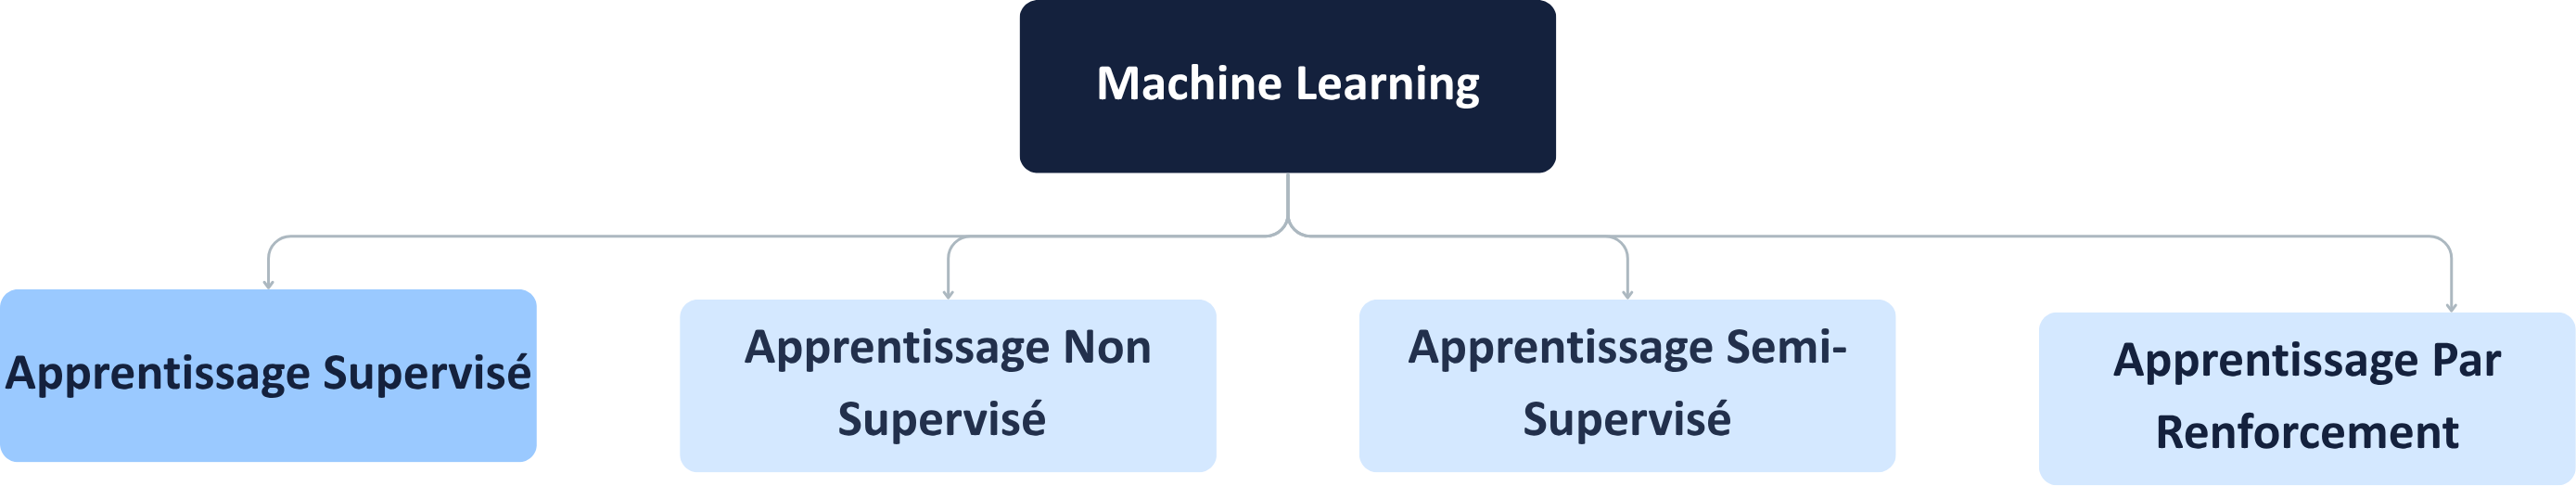
\includegraphics[width=0.85\textwidth]{figures/machinelearningtypes.png}
    \caption{Les quatre familles du Machine Learning.}
    \label{fig:ml-types}
\end{figure}

Dans notre contexte, l'apprentissage \textbf{supervisé} est le seul pertinent~:
nous disposons d'un historique d'exécutions passées (les étiquettes) et l'objectif
est précis : prédire le taux annuel $T4$. Il est important de noter que le ML est
une \textit{branche} de l'intelligence artificielle~: certains systèmes d'IA
fonctionnent par règles écrites manuellement par un expert (on parle de
\textit{systèmes experts}) sans jamais apprendre à partir de données. Dans le
contexte de la prévision budgétaire, où les dynamiques sont trop complexes pour
être encodées à la main, c'est le ML supervisé qui s'impose naturellement.

\paragraph{Le cadre de l'apprentissage supervisé~:}

Dans ce travail, nous utilisons exclusivement l'\textbf{apprentissage supervisé}~: le
modèle apprend à partir d'exemples pour lesquels la «~bonne réponse~» est connue.
Chaque exemple est un couple~:

\begin{itemize}
    \item \textbf{Les variables d'entrée} $\mathbf{x}_i$ (appelées \textit{features})~:
    tout ce qu'on sait \textit{avant} la fin de l'année (taux de réalisation au premier,
    deuxième et troisième trimestre, programme budgétaire, région, part de la ligne dans
    le budget total).
    \item \textbf{La variable à prédire} $y_i$ (appelée \textit{variable cible})~: le
    taux de réalisation annuel final $T4$, connu seulement en fin d'exercice.
\end{itemize}

Le modèle cherche une fonction $f$ telle que $f(\mathbf{x}_i) \approx y_i$~: étant
donné ce qu'on sait en cours d'année, il estime ce que sera le taux final. En termes
formels, l'algorithme minimise une \textbf{fonction de perte} $\mathcal{L}$, qui
mesure l'écart entre la prédiction et la réalité, sur l'ensemble des exemples
historiques~:

$$\hat{f} = \arg\min_{f \in \mathcal{F}} \sum_{i=1}^{n}
\mathcal{L}\bigl(y_i,\, f(\mathbf{x}_i)\bigr)$$

Dans notre application, $\mathcal{L}$ est l'erreur quadratique $(y - \hat{y})^2$, qui
pénalise davantage les grandes erreurs de prédiction.

\paragraph{Comment se déroule un projet de Machine Learning~?}

Un projet de Machine Learning s'inscrit dans un cycle méthodologique structuré, allant
de la collecte des données à leur intégration opérationnelle. Bien que présenté de
manière séquentielle, il convient de souligner d'emblée qu'il s'agit d'un processus
fondamentalement itératif, dans lequel les résultats de chaque phase informent en retour
les décisions prises lors des phases antérieures. Dans le contexte du présent travail,
ce cycle se décline selon les étapes suivantes~:

\begin{enumerate}
    \item \textbf{Collecte des données}~: rassembler des données fiables et
    représentatives. Dans notre cas, il s'agit des rapports trimestriels d'exécution
    budgétaire publiés par la TGR sur la période 2020--2025, complétés par les morasses
    annuelles du ministère de la Justice.
    \item \textbf{Préparation des données}~: nettoyer, structurer et transformer les
    données brutes en un format exploitable par les algorithmes. Cette étape inclut
    la gestion des valeurs manquantes, la création des variables (features) et
    l'encodage des identifiants catégoriels (programme, région).
    \item \textbf{Choix de l'algorithme}~: sélectionner le type de modèle adapté
    au problème. Pour une prévision sur données tabulaires avec historique court,
    Ridge et XGBoost ont été retenus (voir section~3.3).
    \item \textbf{Entraînement du modèle}~: présenter les exemples historiques
    à l'algorithme. Celui-ci ajuste ses paramètres internes pour minimiser l'écart
    entre ses prédictions et les valeurs réelles, selon la formule ci-dessus.
    \item \textbf{Évaluation}~: tester le modèle sur des données qu'il n'a pas
    vues pendant l'entraînement, en mesurant son erreur via le RMSE, le MAE et le
    MAPE. Dans ce travail, cette évaluation se fait par validation walk-forward
    (section~3.4).
    \item \textbf{Amélioration}~: analyser les erreurs commises, ajuster les
    hyperparamètres (profondeur des arbres, taux de régularisation $\lambda$) et
    affiner l'ingénierie des features jusqu'à obtenir des performances satisfaisantes.
    \item \textbf{Déploiement et surveillance}~: intégrer le modèle dans un
    environnement opérationnel et surveiller en continu sa performance sur les
    nouvelles données, en le ré-entraînant si la structure des données évolue.
\end{enumerate}

Ce cycle n'est pas linéaire~: les résultats de l'évaluation conduisent souvent
à revenir sur la préparation des données ou le choix des features. Dans notre
travail, plusieurs itérations ont été nécessaires pour identifier et corriger
les problèmes de fuite de données décrits en section~3.4.

\begin{figure}[h]
    \centering
    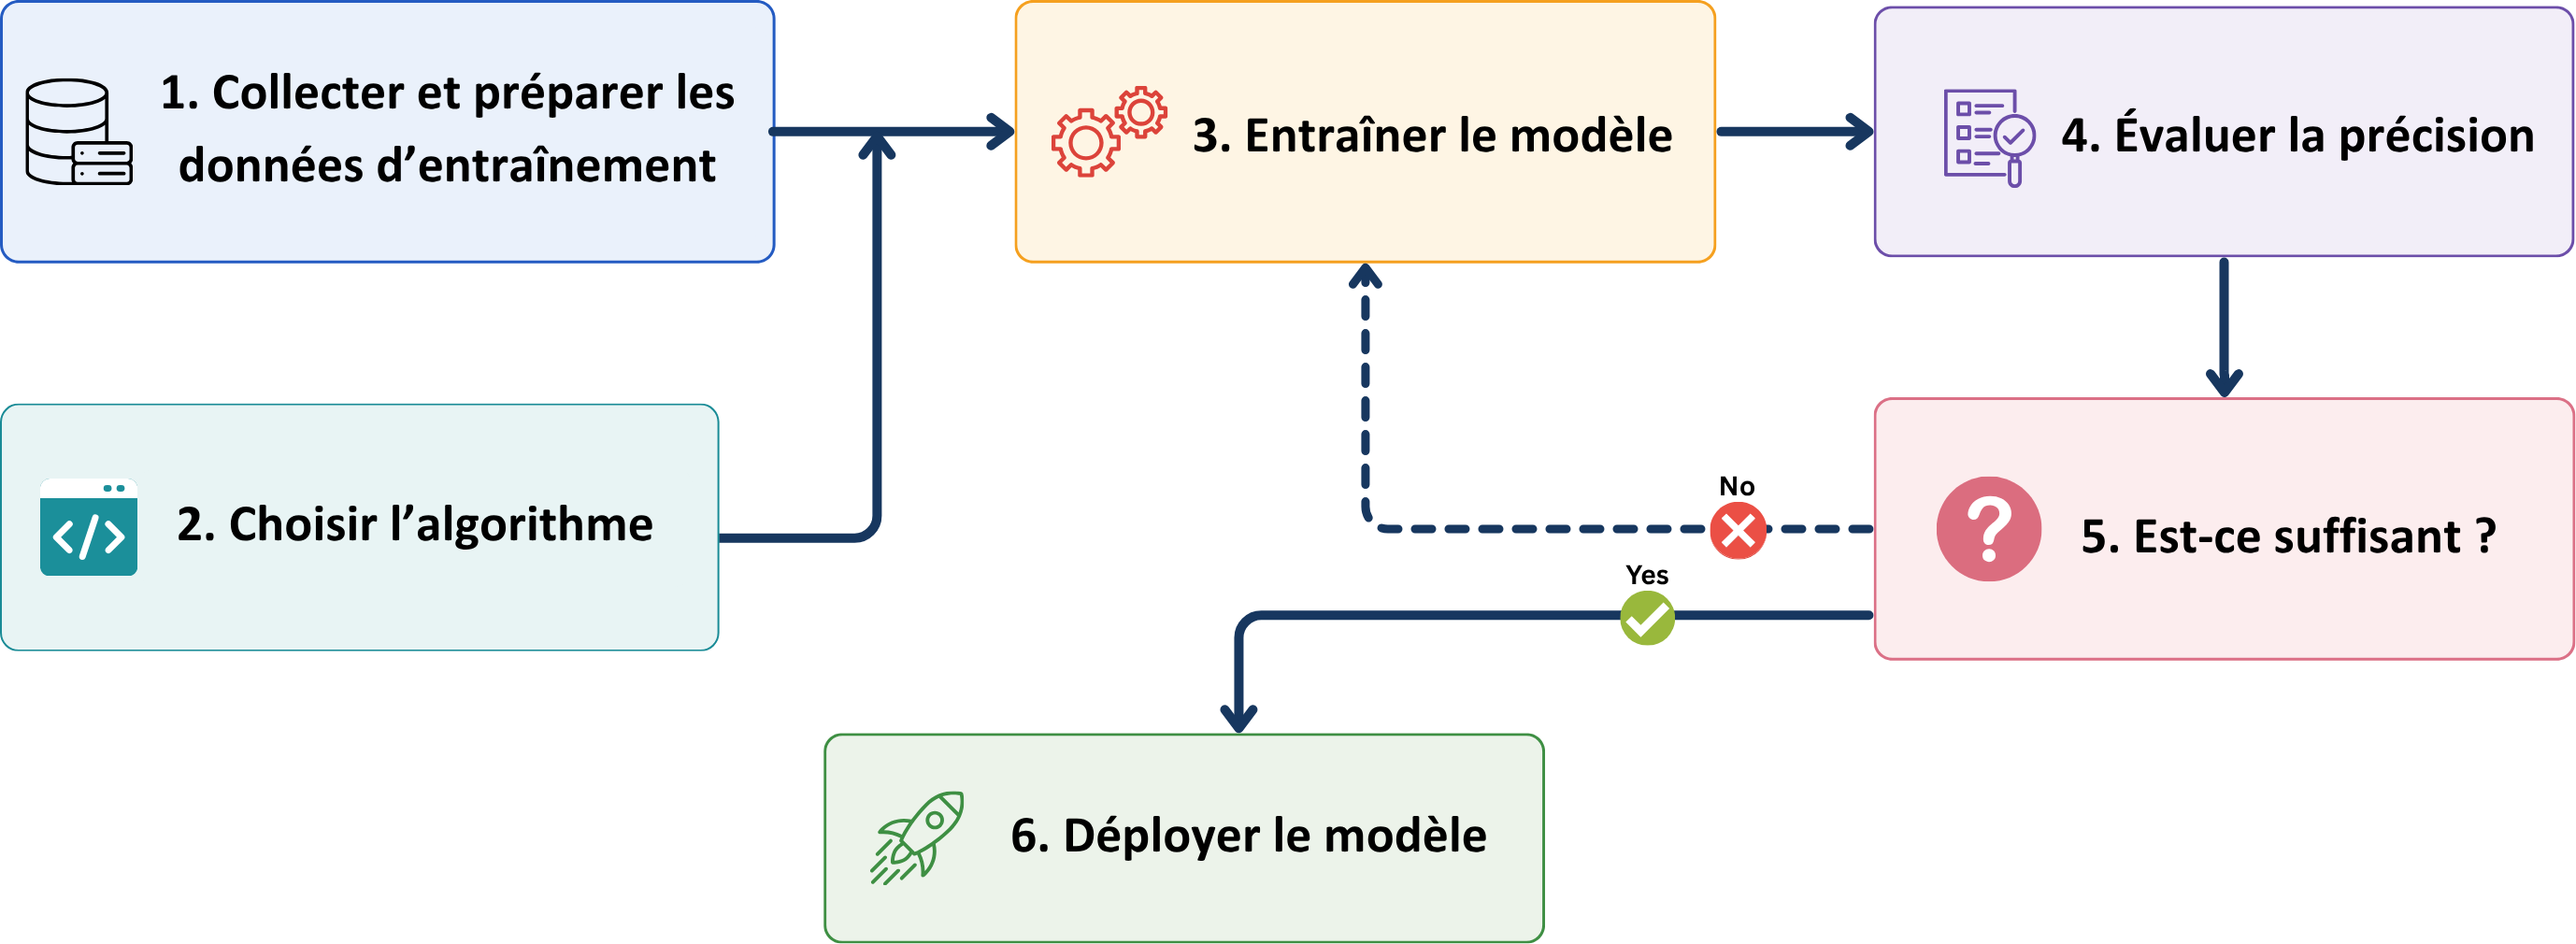
\includegraphics[width=0.85\textwidth]{figures/CommentfonctionneleML.png}
    \caption{Cycle de fonctionnement d'un projet de Machine Learning~: de la
    collecte des données au déploiement, avec itérations d'amélioration.}
    \label{fig:cycle-ml}
\end{figure}

%----------------------------------------------------------------
\phantomsection
\subsubsection*{3.1.2 \quad Pourquoi le Machine Learning}
\addcontentsline{toc}{subsubsection}{3.1.2 Pourquoi le Machine Learning}
%----------------------------------------------------------------

La pr\'evision des taux d'ex\'ecution budg\'etaire pr\'esente trois caract\'eristiques
qui rendent les approches classiques de s\'eries temporelles difficiles \`a appliquer
dans notre contexte~: les comportements sont non lin\'eaires, l'information pertinente
est multidimensionnelle, et l'historique disponible par ligne est court. C'est
pr\'ecis\'ement face \`a ces trois propri\'et\'es que le Machine Learning d\'emontre
le plus clairement sa valeur ajout\'ee.

\paragraph{Non-lin\'earit\'es et effets de seuil~:}

L'ex\'ecution budg\'etaire n'ob\'eit pas \`a une logique de proportionnalit\'e
simple. Une ligne d\'ej\`a \`a 60\,\% de r\'ealisation au deuxi\`eme trimestre
ne se comportera pas du tout de la m\^eme fa\c{c}on qu'une ligne \`a 10\,\%,
m\^eme si l'\'ecart brut avec leur historique respectif est identique. Il existe
des \textbf{effets de seuil et d'acc\'el\'eration}~: au-del\`a d'un certain
niveau d'avancement, la dynamique d'ex\'ecution change de nature. Les algorithmes
ML, en particulier les arbres de d\'ecision (XGBoost), d\'etectent et mod\'elisent
ces ruptures automatiquement, sans qu'on ait besoin de les sp\'ecifier \`a
l'avance.

\paragraph{Int\'egration des variables contextuelles~:}

La capacit\'e d'ex\'ecution d'une ligne budg\'etaire est tributaire d'une multiplicit\'e
de facteurs contextuels~: la cat\'egorie budg\'etaire (Investissement ou Fonctionnement
selon la nature de la d\'epense), le programme de rattachement (Soutien et pilotage,
Performance de l'administration judiciaire, Modernisation du syst\`eme judiciaire et
juridique, ou Renforcement des droits et des libert\'es), la localisation r\'egionale,
la part relative de la ligne dans le budget global, ou encore les profils historiques
de lignes comparables. Les algorithmes ML se distinguent pr\'ecis\'ement par leur capacit\'e
\`a int\'egrer simultan\'ement l'ensemble de ces dimensions et \`a \'etablir, de mani\`ere
automatis\'ee, le poids relatif de chacune d'entre elles selon le type de d\'epense et
l'horizon de pr\'evision consid\'er\'e.

\paragraph{Mutualisation de l'information entre lignes budg\'etaires~:}

Avec seulement 5 \`a 6 ann\'ees d'historique par ligne, tout mod\`ele traitant
chaque ligne s\'epar\'ement travaille sur une base statistique fragile. Le ML
r\'esout ce probl\`eme en \textbf{agr\'egeant toutes les lignes et toutes les
ann\'ees dans un seul jeu d'entra\^inement}~: une ligne qui n'a que 5 ann\'ees
d'historique b\'en\'eficie des patterns observ\'es sur l'ensemble du panel. Le
mod\`ele apprend des r\`egles transversales~: par exemple, que les lignes
d'investissement en retard \`a mi-ann\'ee rattrapent en g\'en\'eral leur d\'eficit
au quatri\`eme trimestre, ou que les lignes de fonctionnement \`a forte part
budg\'etaire sont structurellement pr\'evisibles. Cette mutualisation est l'un
des avantages les plus d\'ecisifs de l'approche dans notre contexte.

\vspace{4pt}
Le tableau suivant synth\'etise ces propri\'et\'es~:

\begin{table}[h]
\centering
\caption{Comparaison des m\'ethodes classiques et des approches de Machine Learning.}
\label{tab:comparaison-ml}
\begin{tabular}{lll}
\hline
\textbf{Propri\'et\'e} & \textbf{M\'ethodes classiques}
& \textbf{ML (Ridge / XGBoost)} \\
\hline
Non-linéarités et effets de seuil & Non & Oui \\
Variables contextuelles multiples & Limité & Naturellement intégrées \\
Courtes séries par ligne & Fragile & Robuste (mutualisation) \\
Interprétabilité & Coefficients & Coefficients (Ridge), importance (XGB) \\
\hline
\end{tabular}
\end{table}

%----------------------------------------------------------------
\phantomsection
\subsubsection*{3.1.3 \quad Limites des approches classiques de prévision}
\addcontentsline{toc}{subsubsection}{3.1.3 Limites des approches classiques de prévision}
%----------------------------------------------------------------

Le chapitre~2 a recensé les principales méthodes de prévision utilisées dans la
littérature budgétaire~: modèles ARIMA/SARIMA, régressions saisonnières, lissages
exponentiels. Ces approches reposent sur des hypothèses qui se révèlent difficiles
à satisfaire dans notre contexte.

Premièrement, elles exigent des séries temporelles suffisamment longues par entité
prédite~: ARIMA recommande au moins 50 observations pour une estimation fiable, ce
qui correspond à plus de 12 années de données trimestrielles par ligne. Avec
seulement 5 à 6 ans d'historique, l'estimation des paramètres est instable et les
intervalles de confiance très larges.

Deuxièmement, ces méthodes traitent chaque ligne budgétaire de façon isolée~: elles
ne peuvent pas exploiter le fait que des lignes relevant du même programme ou de
la même région partagent des dynamiques communes. L'information potentiellement
précieuse contenue dans les centaines de lignes du budget n'est pas mutualisée.

Troisièmement, l'intégration de variables contextuelles explicatives (programme,
région, indicateurs judiciaires) dans un modèle ARIMA requiert des extensions
ARIMAX qui augmentent considérablement sa complexité sans garantir une amélioration
sensible des performances quand l'historique est court. Ces limites motivent le
recours au Machine Learning, dont les apports spécifiques à notre contexte ont été
présentés en section~3.1.2.

%================================================================
\phantomsection
\subsection*{3.2 \quad Apprentissage supervisé}
\addcontentsline{toc}{subsection}{3.2 Apprentissage supervisé}
%================================================================

%----------------------------------------------------------------
\phantomsection
\subsubsection*{3.2.1 \quad Généralisation}
\addcontentsline{toc}{subsubsection}{3.2.1 Généralisation}
%----------------------------------------------------------------

Un modèle ML n'a de valeur que s'il prédit correctement des situations qu'il n'a
\textit{jamais vues}. Or un algorithme suffisamment puissant peut «~mémoriser~»
tous ses exemples d'entraînement sans réellement comprendre les patterns sous-jacents.
Ce phénomène s'appelle le \textbf{surapprentissage} (\textit{overfitting})~: le
modèle performe brillamment sur ses données d'entraînement et échoue sur de
nouvelles données. La \textbf{généralisation} désigne précisément la capacité d'un
modèle à maintenir ses performances sur des données inédites, critère
déterminant pour un usage opérationnel.

La généralisation dépend d'un équilibre délicat entre la complexité du modèle et
la quantité de données disponibles. Un modèle trop simple ne captera pas les
patterns importants~; un modèle trop complexe les mémorisera sans les comprendre.
Cet équilibre est formalisé par le compromis biais-variance.

%----------------------------------------------------------------
\phantomsection
\subsubsection*{3.2.2 \quad Le compromis biais-variance}
\addcontentsline{toc}{subsubsection}{3.2.2 Le compromis biais-variance}
%----------------------------------------------------------------

L'erreur totale d'un modèle peut toujours se décomposer en trois termes~:

$$\text{Erreur totale} = \underbrace{\text{Biais}^2}_{\text{modèle trop simple}}
+ \underbrace{\text{Variance}}_{\text{modèle trop complexe}}
+ \text{Bruit irréductible}$$

\begin{itemize}
    \item Le \textbf{biais} traduit un \textit{sous-apprentissage}~: le modèle est
    trop simple et rate des patterns importants. Exemple~: supposer que le taux final
    est toujours égal au taux du deuxième trimestre.
    \item La \textbf{variance} traduit un \textit{surapprentissage}~: le modèle est
    trop complexe et apprend le bruit au lieu du signal. Il s'adapte parfaitement à
    l'historique, mais généralise mal.
    \item Le \textbf{bruit irréductible}~: une partie de la réalité est par nature
    imprévisible (décisions politiques de dernière minute, suspensions de dépenses
    imprévues, événements exceptionnels). Aucun modèle ne peut l'éliminer.
\end{itemize}

Les métriques d'évaluation quantifient cet écart entre prédictions et réalité.
Trois indicateurs sont utilisés dans ce travail~:

$$\text{RMSE} = \sqrt{\frac{1}{n}\sum_{i=1}^{n}(y_i - \hat{y}_i)^2} \qquad
\text{MAE} = \frac{1}{n}\sum_{i=1}^{n}|y_i - \hat{y}_i| \qquad
\text{MAPE} = \frac{100}{n}\sum_{i=1}^{n}\left|\frac{y_i - \hat{y}_i}{y_i}\right|\,\%$$

\begin{itemize}
    \item Le \textbf{RMSE} (Racine de l'Erreur Quadratique Moyenne) est la métrique
    principale. Il pénalise plus fortement les grandes erreurs~: se tromper de 20\,\%
    est bien pire que deux erreurs de 10\,\%.
    \item Le \textbf{MAE} (Erreur Absolue Moyenne) donne l'erreur typique en valeur
    absolue, moins sensible aux cas exceptionnels.
    \item Le \textbf{MAPE} (Erreur Absolue Moyenne en Pourcentage) exprime l'erreur
    en pourcentage, ce qui facilite la comparaison entre lignes de niveaux très
    différents.
\end{itemize}

Dans notre protocole, le RMSE sert de critère principal de sélection des modèles~;
MAE et MAPE sont présentés en complément dans les tableaux du chapitre~4.

%----------------------------------------------------------------
\phantomsection
\subsubsection*{3.2.3 \quad Surapprentissage et robustesse}
\addcontentsline{toc}{subsubsection}{3.2.3 Surapprentissage et robustesse}
%----------------------------------------------------------------

Avec seulement 5 à 6 années d'historique par ligne, un modèle très complexe risque
fortement de mémoriser les données plutôt que d'en extraire des règles généralisables.
Nous privilégions donc des modèles \textbf{régularisés} (Lasso et XGBoost avec
pénalités $L_1/L_2$) qui incluent un mécanisme interne limitant leur propre
complexité, trouvant ainsi le bon équilibre entre simplicité et précision.

Trois contraintes spécifiques à notre contexte plafonnent par ailleurs la précision
atteignable~:

\begin{enumerate}
    \item \textbf{Volume de données limité}~: cinq à six années d'historique par ligne
    représentent un volume modeste. Les modèles à grand nombre de paramètres risquent
    de mémoriser ces quelques exemples plutôt que d'en extraire des règles robustes.

    \item \textbf{Données partiellement synthétiques}~: les taux d'exécution publiés
    par la Trésorerie Générale du Royaume (TGR) sont des agrégats par catégorie, sans
    ventilation par programme ni par région. La construction du panel désagrégé repose
    donc sur une simulation calibrée (décrite au chapitre~4), ce qui introduit une
    imprécision structurelle dans les données d'entraînement.

    \item \textbf{Variables non observables}~: certains facteurs qui influencent
    l'exécution budgétaire ne figurent tout simplement pas dans les données : une
    décision de suspendre temporairement des dépenses en cours d'année, un retard
    dans le lancement d'un appel d'offres, ou une réallocation de crédits d'un
    programme vers un autre décidée au niveau central. Ces événements, invisibles
    pour le modèle, peuvent pourtant modifier significativement le niveau de
    consommation observé en fin d'année. Même le meilleur algorithme ne peut pas
    prédire ce qu'il ne voit pas.
\end{enumerate}

%================================================================
\phantomsection
\subsection*{3.3 \quad Les modèles retenus}
\addcontentsline{toc}{subsection}{3.3 Les modèles retenus}
%================================================================

Quatre modèles ont été évalués dans ce travail~: deux \textbf{benchmarks naïfs}
(sans apprentissage statistique) qui servent de barre minimale, et deux
\textbf{algorithmes ML} à proprement parler. Le choix a été guidé par deux critères~:
la pertinence théorique face aux données budgétaires, et la faisabilité d'un
déploiement réel dans une administration publique (un modèle trop opaque ou trop
coûteux à maintenir n'a pas de valeur opérationnelle).

%----------------------------------------------------------------
\phantomsection
\subsubsection*{3.3.1 \quad Modèles de référence (benchmarks naïfs)}
\addcontentsline{toc}{subsubsection}{3.3.1 Modèles de référence (benchmarks naïfs)}
%----------------------------------------------------------------

Avant l'introduction de tout modèle sophistiqué, il convient d'établir des références
méthodologiques simples~: des prévisions qu'un gestionnaire pourrait produire sans recours
à des techniques avancées, et qui constituent dès lors la borne minimale que tout modèle
de Machine Learning se doit de surpasser pour justifier sa complexité additionnelle.

\paragraph{Benchmark 1~: Moyenne historique~:}

Le benchmark le plus élémentaire repose sur l'extrapolation directe de la performance
historique~: si une ligne a réalisé en moyenne 82\,\% de son enveloppe annuelle au cours
des cinq derniers exercices, on projette ce même taux d'exécution pour l'année en cours.

$$\hat{y}_i = \frac{1}{N} \sum_{t=1}^{N} y_{i,t}$$

\noindent\small\textit{où $\hat{y}_i$ est la prévision pour la ligne $i$, $N$ le nombre d'années d'entraînement, et $y_{i,t}$ le taux d'exécution réel de la ligne $i$ en année $t$.}\normalsize

Ce benchmark capture la \textbf{persistance structurelle} du taux d'exécution~:
certaines lignes sont structurellement bien exécutées, d'autres chroniquement
sous-exécutées. Ignorer cet historique serait une erreur.

\paragraph{Benchmark 2~: Naïf saisonnier lag-4~:}

Une variante alternative consiste à projeter, pour l'année courante, le taux d'exécution
exactement réalisé lors de l'exercice antérieur.

$$\hat{y}_i = y_{i,\, Y-1}$$

\noindent\small\textit{où $y_{i,\, Y-1}$ est le taux d'exécution réel de la ligne $i$ l'année précédente.}\normalsize

Ce benchmark s'avère souvent difficile à surpasser en pratique, dans la mesure où il
capture implicitement les phénomènes d'inertie institutionnelle et les tendances récentes
de la dynamique budgétaire. Par conséquent, un modèle de Machine Learning incapable de
produire des prévisions plus fiables que cette simple reconduction n'apporte aucune
valeur ajoutée opérationnelle.

Ces deux benchmarks constituent la \textbf{barre minimale} que les modèles ML doivent
franchir pour justifier leur déploiement.

%----------------------------------------------------------------
\phantomsection
\subsubsection*{3.3.2 \quad Ridge (régularisation)}
\addcontentsline{toc}{subsubsection}{3.3.2 Ridge (régularisation)}
%----------------------------------------------------------------

\paragraph{Principe en langage clair~:}

La régression linéaire classique cherche la combinaison de variables qui prédit le
mieux le taux final~: «~le taux final vaut approximativement $a$ fois le taux T2,
plus $b$ fois la part budgétaire, plus une constante~». Le problème~: avec beaucoup
de variables et peu d'observations, le modèle peut attribuer des coefficients
aberrants à des variables peu informatives, ce qui nuit à la généralisation.

Le \textbf{Ridge} (Tikhonov regularization) ajoute une contrainte~: les coefficients
trop grands sont pénalisés. Contrairement au Lasso qui force certains coefficients
à zéro, Ridge réduit progressivement tous les coefficients vers zéro sans les
éliminer complètement. Cela produit un modèle plus stable et robuste, particulièrement
utile en présence de données avec outliers.

$$\min_{\beta_1,\ldots,\beta_p} \;\; \underbrace{\frac{1}{n}\sum_{i=1}^{n}(y_i - \hat{y}_i)^2}_{\text{erreur de prédiction}} \;+\; \lambda \underbrace{\sum_{j=1}^{p}\beta_j^2}_{\text{pénalité L2 sur les coefficients}}$$

\noindent\small\textit{Les $\beta_j$ sont les coefficients du modèle. $\lambda$ est choisi par validation croisée.}\normalsize

Le paramètre $\lambda$ contrôle l'intensité de cette contrainte~: plus $\lambda$ est
grand, plus les coefficients sont réduits. Sa valeur est choisie automatiquement par
validation croisée (voir section~3.4).

\paragraph{Pourquoi Ridge pour les dépenses de matériel~?}

Les dépenses de matériel et dépenses diverses ont un profil d'exécution
\textbf{régulier et prévisible}, avec peu de variation d'une année à l'autre. Dans
ce contexte, l'hypothèse de linéarité est raisonnable. Ridge est particulièrement
adapté car (1) il limite le surapprentissage sur peu de données, (2) il conserve
tous les prédicteurs même faibles, ce qui améliore la stabilité face aux outliers,
et (3) ses résultats restent interprétables~: un gestionnaire peut comprendre qu'
«~une hausse d'un point de pourcentage du taux au deuxième trimestre se traduit par
une hausse de $\beta_{T2}$ points du taux annuel final~».

\textbf{Note sur la normalisation~:} Les variables d'entrée doivent être normalisées avant
d'être soumises à Ridge. Deux stratégies sont possibles~: le \textit{StandardScaler},
fondé sur la moyenne et l'écart-type (optimal pour distributions gaussiennes, sensible
aux valeurs extrêmes), ou le \textit{RobustScaler}, fondé sur la médiane et l'intervalle
interquartile (plus robuste en présence d'outliers). Le choix dépend de la structure
des données. Dans ce travail, le \textit{RobustScaler} s'est révélé supérieur sur
les dépenses de matériel car il neutralise les anomalies de courte durée (voir
section 4.5.5 pour les détails d'optimisation post-validation).

%----------------------------------------------------------------
\phantomsection
\subsubsection*{3.3.3 \quad Méthodes d'ensemble (XGBoost)}
\addcontentsline{toc}{subsubsection}{3.3.3 Méthodes d'ensemble (XGBoost)}
%----------------------------------------------------------------

\paragraph{Principe en langage clair~:}

Le \textbf{gradient boosting} repose sur un principe de correction itérative des erreurs
mis en œuvre par un ensemble séquentiel de modèles faibles~: un premier modèle produit
une estimation initiale~; chaque modèle subséquent se concentre spécifiquement sur la
correction des résidus engendrés par les précédents. Cette approche cumulative, par laquelle
l'ensemble des corrections successives s'agrègent, conduit à une prévision globale
sensiblement plus fidèle que celle qu'aurait pu fournir un modèle unique considéré
isolément.

Dans XGBoost, chaque «~expert~» est un \textbf{arbre de décision}~: une suite de
questions simples du type «~est-ce que le taux T2 est supérieur à 45\,\%~?~» qui
débouche sur une prévision. L'algorithme construit une séquence d'arbres
$T_1, T_2, \ldots, T_K$, chacun corrigeant les erreurs du précédent~:

$$\underbrace{\hat{y}_i^{(k)}}_{\text{nouvelle pr\'evision}} = \underbrace{\hat{y}_i^{(k-1)}}_{\text{pr\'evision pr\'ec\'edente}} + \eta \cdot \underbrace{T_k(x_i)}_{\text{correction de l'arbre }k}$$

où $\eta$ est un «~taux d'apprentissage~» qui contrôle à quel point chaque correctif
est appliqué (une valeur faible rend l'apprentissage plus prudent). La prévision
finale est la somme de tous les arbres~:

$$\hat{y}_i = \sum_{k=1}^{K} \eta \cdot T_k(x_i)$$

Pour éviter le surapprentissage, chaque arbre est contraint dans sa complexité par
des paramètres de régularisation~: limite sur la profondeur des arbres, pénalités
sur les feuilles, et sous-échantillonnage aléatoire des données à chaque étape.

\paragraph{Pourquoi XGBoost pour les dépenses d'investissement~?}

Le choix de XGBoost pour les dépenses d'investissement se fonde sur une observation
empirique déterminante~: les dynamiques d'exécution de cette catégorie présentent des
\textbf{non-linéarités prononcées}. À titre d'illustration, une ligne dont le taux
d'exécution s'établit à 5\,\% au deuxième trimestre, rattachée à un programme
d'investissement en infrastructure, peut atteindre 80\,\% en clôture d'exercice grâce
à des décaissements massifs concentrés en fin d'année --- phénomène qu'un modèle
linéaire ne saurait anticiper. XGBoost s'avère particulièrement adapté à ce type de
configuration, et ce pour les raisons suivantes~:

\begin{itemize}
    \item Il capture naturellement les \textbf{effets de seuil et les interactions}~:
    l'effet du taux T2 peut être différent selon le programme, la région ou la taille
    de la ligne.
    \item Il \textbf{généralise bien avec peu de données}~: contrairement aux réseaux
    de neurones, XGBoost est efficace avec quelques centaines d'observations grâce à
    sa régularisation intégrée.
    \item Il est \textbf{interprétable}~: l'importance de chaque variable (combien elle
    contribue en moyenne aux prédictions) peut être extraite et présentée à des
    gestionnaires non-spécialistes.
    \item Il est \textbf{open-source et rapide}~: déployable sans licence commerciale,
    son exécution sur un ordinateur de bureau standard prend quelques secondes,
    un impératif dans un contexte ministériel.
\end{itemize}

%----------------------------------------------------------------
\phantomsection
\subsubsection*{3.3.4 \quad Couche de détection d'anomalies}
\addcontentsline{toc}{subsubsection}{3.3.4 Couche de détection d'anomalies}
%----------------------------------------------------------------

En complément des prévisions, le système intègre une \textbf{couche de détection
d'anomalies de sous-exécution}. Le principe est simple~: \textit{le système calcule
un score Z par ligne, comparant son taux d'exécution T2 à sa propre moyenne
historique. Une déviation de plus de 1,5~écarts-types déclenche une alerte
opérationnelle.} Formellement, pour chaque ligne budgétaire $i$, on calcule un
\textbf{score Z} comme suit~:

$$z_i = \frac{\text{taux}_{i,\text{T2}} - \mu_i}{\sigma_i}$$

\noindent\small\textit{où $\mu_i$ et $\sigma_i$ sont la moyenne et l'écart-type du
taux T2 de la ligne $i$ sur les années d'entraînement.}\normalsize

Une ligne est \textbf{signalée comme anomalie} si $z_i < -1{,}5$, ce qui indique
que son niveau d'exécution à mi-année est statistiquement anormal par rapport à
son propre historique. Trois niveaux de sévérité sont distingués~:

\begin{itemize}
    \item \textbf{Exécution nulle}~: taux T2~$= 0$, aucun décaissement enregistré~;
    \item \textbf{Sous-exécution sévère}~: $z_i < -2$, écart très inhabituel~;
    \item \textbf{Sous-exécution modérée}~: $-2 \leq z_i < -1{,}5$, signal d'alerte préventive.
\end{itemize}

Cette couche ne constitue \textit{pas} une détection de fraude au sens pénal~: elle
identifie des \textbf{anomalies opérationnelles} -- lignes bloquées administrativement,
crédits non encore délégués, ou projets n'ayant pas démarré -- qui nécessitent une
intervention de pilotage avant la clôture de l'exercice.

%----------------------------------------------------------------
\phantomsection
\subsubsection*{3.3.5 \quad Justification des modèles écartés}
\addcontentsline{toc}{subsubsection}{3.3.5 Justification des modèles écartés}
%----------------------------------------------------------------

\paragraph{Principe~:}

Le Random Forest fonctionne lui aussi sur le principe d'une «~équipe d'arbres~»,
mais différemment~: au lieu de travailler en séquence (chacun corrigeant le
précédent), les arbres travaillent \textbf{en parallèle et indépendamment}, chacun
entraîné sur un sous-ensemble aléatoire des données. La prévision finale est la
moyenne de toutes leurs réponses~:

$$\hat{y}_i = \frac{1}{B} \sum_{b=1}^{B} \underbrace{T_b(x_i)}_{\text{r\'eponse de l'arbre }b}$$

\noindent\small\textit{$B$ arbres votent ind\'ependamment~; la pr\'evision finale est leur moyenne.}\normalsize

Cette indépendance réduit le risque de surapprentissage, mais elle a un coût~: les
arbres ne se corrigent pas mutuellement, ce qui les rend moins précis individuellement.

\paragraph{Pourquoi Lasso a été écarté~:}

Lasso (Least Absolute Shrinkage and Selection Operator) a initialement été considéré
pour prédire les dépenses de matériel, car il offre une sélection automatique des
prédicteurs. Cependant, la validation walk-forward a révélé ses limitations~:

\begin{enumerate}
    \item \textbf{Sensibilité aux outliers}~: Le mécanisme de sélection (force
    certains coefficients à zéro) peut ètre fragilisé par quelques valeurs extrêmes,
    conduisant à des modèles instables d'une année à l'autre.
    \item \textbf{Ridge plus stable}~: Ridge (Régularisation L2) réduit progressivement
    tous les coefficients sans les éliminer, produisant une meilleure stabilité
    face aux outliers par normalisation avec RobustScaler.
    \item \textbf{Performance empirique}~: Sur les données du ministère de la Justice,
    Ridge + RobustScaler a surpassé Lasso + StandardScaler de 9,1~points de RMSE
    (voir section 4.5.5).
\end{enumerate}

Lasso est néanmoins documenté dans les tableaux de comparaison du chapitre~4 comme
algorithme initialement testé ; sa évaluation comparative appuie la pertinence du
choix de Ridge pour ce contexte.

\paragraph{Pourquoi Random Forest a été écarté~:}

Random Forest a été évalué lors de la validation walk-forward (détaillée au
chapitre~4), mais n'a pas été retenu comme modèle de production, pour trois raisons~:

\begin{enumerate}
    \item \textbf{Performances inférieures}~: XGBoost a systématiquement produit des
    erreurs plus faibles sur les dépenses d'investissement, la catégorie la plus
    complexe. L'entraînement sur des sous-échantillons aléatoires peut éliminer
    des patterns utiles quand les données sont rares.
    \item \textbf{Incapacité à extrapoler}~: les arbres de décision ne peuvent pas
    prédire au-delà des valeurs observées pendant l'entraînement. Pour des lignes
    dont les taux 2025 dépassent tous les niveaux historiques, Random Forest plafonne
    méchaniquement, tandis que XGBoost peut s'ajuster prudemment.
    \item \textbf{Parcimonie opérationnelle}~: dans un contexte de déploiement réel,
    retenir le modèle le plus performant par catégorie est préférable à empiler
    plusieurs algorithmes dans un ensemble hybride difficile à expliquer et à maintenir.
\end{enumerate}

Random Forest est néanmoins présenté dans les tableaux de résultats du chapitre~4
comme point de comparaison ; sa mise en concurrence avec les autres modèles est un
élément de rigueur méthodologique essentiel.

%================================================================
\phantomsection
\subsection*{3.4 \quad La validation rigoureuse}
\addcontentsline{toc}{subsection}{3.4 La validation rigoureuse}
%================================================================

Construire un modèle ML n'est que la moitié du travail. L'autre moitié consiste à
\textbf{mesurer honnêtement sa performance}~: combien d'erreur fait-il sur des
données qu'il n'a jamais vues~? Cette question semble simple, mais elle cache un
piège redoutable dans le contexte des séries temporelles.

%----------------------------------------------------------------
\phantomsection
\subsubsection*{3.4.1 \quad Les données temporelles}
\addcontentsline{toc}{subsubsection}{3.4.1 Les données temporelles}
%----------------------------------------------------------------

\paragraph{La validation croisée standard~: efficace mais inadaptée ici~:}

La validation croisée en $k$ groupes (\textit{k-fold}) constitue la méthode standard
d'évaluation des modèles de Machine Learning~: l'ensemble des données est partitionné
en $k$ sous-ensembles disjoints~; à chaque itération, l'un de ces sous-ensembles est
réservé au test, tandis que le modèle est entraîné sur les $k-1$ sous-ensembles
restants. La performance globale est alors estimée par la moyenne des erreurs sur
l'ensemble des folds.

\begin{table}[h]
\centering
\caption{Sch\'ema de la validation crois\'ee $k$-fold (exemple~: Groupe~2 = test).}
\label{tab:kfold}
\begin{tabular}{|c|c|c|c|c|}
\hline
\textbf{Groupe 1} & \cellcolor{primary!40}\textbf{Groupe 2} & \textbf{Groupe 3} & \textbf{Groupe 4} & \textbf{Groupe 5} \\
\hline
Entr. & \textbf{Test} & Entr. & Entr. & Entr. \\
\hline
\end{tabular}\\[4pt]
{\scriptsize Groupe 2 = test~; groupes 1, 3, 4, 5 = entra\^inement}
\end{table}

Si cette approche demeure valide lorsque les observations satisfont l'hypothèse
d'indépendance mutuelle, son application à des données temporelles introduit un biais
méthodologique critique~: la permutation aléatoire des années au sein des groupes de
validation autorise le modèle à accéder, lors de son entraînement, à des informations
postérieures à la période qu'il est censé prédire. Autrement dit, un modèle ayant
«~observé~» les réalisations de 2024 pour prédire celles de 2022 bénéficie d'une
divulgation implicite d'information temporelle, ce qui invalide dès lors la mesure de
sa capacité prédictive réelle.

\paragraph{La contrainte fondamentale~: toujours prédire vers l'avant~:}

Pour les séries temporelles, une règle doit être respectée absolument~: les données
d'entraînement doivent toujours être antérieures aux données de test. Cela donne
naissance à des protocoles de validation spécifiques.

%----------------------------------------------------------------
\phantomsection
\subsubsection*{3.4.2 \quad Validation walk-forward}
\addcontentsline{toc}{subsubsection}{3.4.2 Validation walk-forward}
%----------------------------------------------------------------

Le protocole retenu dans ce travail est la \textbf{validation walk-forward à fenêtre
expansive}, qui reproduit fidèlement le cadre opérationnel auquel se trouvera confronté
le décideur en conditions réelles. Concrètement~:

\begin{itemize}
    \item Pour prédire l'année 2022, le modèle s'entraîne uniquement sur 2020--2021.
    \item Pour prédire 2023, il s'entraîne sur 2020--2022.
    \item Pour prédire 2024, il s'entraîne sur 2020--2023.
    \item Pour prédire 2025, il s'entraîne sur 2020--2024.
\end{itemize}

La caractéristique centrale de cette approche réside dans l'élargissement progressif
de la fenêtre d'entraînement à chaque étape temporelle, reflétant l'accumulation
naturelle d'expérience historique au fil du temps. Ainsi, plus l'horizon de prévision
se rapproche du présent, plus le modèle bénéficie d'un volume substantiel de données
antérieures. La performance globale est in fine estimée en moyennant les erreurs commises
sur les quatre périodes de test ainsi définies.

\begin{table}[h]
\centering
\setlength{\tabcolsep}{4pt}
\caption{Protocole de validation walk-forward \`a fen\^etre expansive (2022--2025).}
\label{tab:walkforward}
\begin{tabular}{l|ccccc}
\hline
 & \textbf{2021} & \textbf{2022} & \textbf{2023} & \textbf{2024} & \textbf{2025} \\
\hline
Fold 1 (test 2022) & \cellcolor{accent!30}Entr. & \cellcolor{primary!40}\textbf{Test} & & & \\
Fold 2 (test 2023) & \cellcolor{accent!30}Entr. & \cellcolor{accent!30}Entr. & \cellcolor{primary!40}\textbf{Test} & & \\
Fold 3 (test 2024) & \cellcolor{accent!30}Entr. & \cellcolor{accent!30}Entr. & \cellcolor{accent!30}Entr. & \cellcolor{primary!40}\textbf{Test} & \\
Fold 4 (test 2025) & \cellcolor{accent!30}Entr. & \cellcolor{accent!30}Entr. & \cellcolor{accent!30}Entr. & \cellcolor{accent!30}Entr. & \cellcolor{primary!40}\textbf{Test} \\
\hline
\end{tabular}\\[4pt]
{\scriptsize \colorbox{accent!30}{\strut Entra\^inement} \quad
\colorbox{primary!40}{\strut Test} \quad Cases vides = donn\'ees non encore disponibles}
\end{table}

Ce protocole présente trois avantages majeurs~:

\begin{itemize}
    \item \textbf{Simulation exacte du déploiement réel}~: chaque fold reproduit
    fidèlement la situation du gestionnaire : il dispose de tout l'historique passé
    et prédit l'année courante.
    \item \textbf{Aucune contamination temporelle}~: à aucun moment le modèle n'est
    entraîné sur des données postérieures à l'année qu'il prédit.
    \item \textbf{Mesure de la progression}~: comparer les erreurs du fold 2022 (peu
    de données) à celles du fold 2025 (plus de données) quantifie l'apport de chaque
    année d'historique supplémentaire.
\end{itemize}

%----------------------------------------------------------------
\phantomsection
\subsubsection*{3.4.3 \quad Risque de data leakage}
\addcontentsline{toc}{subsubsection}{3.4.3 Risque de data leakage}
%----------------------------------------------------------------

\paragraph{Qu'est-ce que la fuite de données~?}

La \textbf{fuite de données} (\textit{data leakage}) est une erreur qui consiste à
laisser entrer dans le processus d'entraînement des informations qui ne seraient pas
disponibles au moment d'une vraie prévision. Le modèle apprend alors des patterns
«~trop faciles~» qui disparaissent en production. Le symptôme est trompeur~: les
métriques de validation semblent excellentes, mais le modèle déçoit une fois déployé.

\paragraph{Mécanisme 1~: fuite par le protocole de validation~:}

Si le jeu de test est l'année~2022 mais que le modèle s'entraîne sur des données
incluant 2023, 2024 et 2025, il «~voit l'avenir~» pendant l'entraînement. La méthode
LOYO (\textit{Leave-One-Year-Out}) commet exactement cette erreur~: pour tester 2022,
elle entraîne sur toutes les autres années y compris les années ultérieures, ce qui
produit des métriques artificiellement optimistes. Le walk-forward élimine ce risque
par construction.

\paragraph{Mécanisme 2~: fuite par les variables explicatives~:}

Même avec un bon protocole, la fuite peut s'introduire lors de la construction des
variables. Exemple typique~: si on calcule «~la moyenne historique des taux T3 de
cette ligne sur toutes les années disponibles~» et qu'on l'utilise pour prédire 2022,
cette moyenne inclut les années 2023, 2024, 2025, soit des données futures. La solution
est de calculer cette moyenne de façon \textbf{causale}~: pour prédire l'année $Y$,
n'utiliser que les années strictement antérieures à $Y$.

%----------------------------------------------------------------
\phantomsection
\subsubsection*{3.4.4 \quad Prévision directe vs roulante}
\addcontentsline{toc}{subsubsection}{3.4.4 Prévision directe vs roulante}
%----------------------------------------------------------------

\paragraph{Motivation pratique~:}

La validation walk-forward présentée en section~3.4.2 garantit une séparation temporelle
stricte~: le modèle ne voit jamais d'information future. Cependant, cette approche
reflète un scénario académique où l'on prédisait à~$t=0$ l'intégralité d'une année
budgétaire sans aucune donnée intra-annuelle.

En réalité, les gestionnaires budgétaires ne prédisent pas deux ans à l'avance~: ils
ont besoin de réviser les prévisions en cours d'exécution. Par exemple, à la mi-année
(T2 écoulé), on dispose déjà des taux d'exécution réels pour T1 et T2, et l'enjeu est
de prédire le taux final T4. Cette situation est fondamentalement différente, car elle
combine~:
\begin{enumerate}
  \item Une \textbf{fenêtre d'observation}~: données passées réelles (T1, T2)
  \item Une \textbf{fenêtre de prédiction}~: données futures inconnues (T4)
  \item Une \textbf{fenêtre intermédiaire}~: T3, potentiellement prédite ou observée
\end{enumerate}

\paragraph{Deux stratégies de prédiction~:}

\textbf{Approche directe~:} Le modèle reçoit directement T1 et T2 observés comme entrées
et produit en un seul passage la prédiction de T4 finale. Cette approche suppose que la
relation $(T1, T2) \to T4$ peut être apprise directement depuis les données historiques,
sans étape intermédiaire.

\textbf{Approche roulante~:} Le processus de prédiction se décompose en deux étapes
séquentielles~:
\begin{enumerate}
  \item \textbf{Étape 1~:} Prédire T3 à partir de T1 et T2 observés
  \item \textbf{Étape 2~:} Prédire T4 à partir de T1, T2 observés \textit{et} T3 prédit
\end{enumerate}

L'approche roulante capture une structure temporelle progressive~: on suppose que T3 est
informatif pour prédire T4, et que les modèles bénéficient de cette information
intermédiaire, même si elle est elle-même entachée d'erreur de prédiction.

\paragraph{Implications méthodologiques~:}

Cette distinction revêt une importance capitale pour la conception du système de
prévision. Alors que la validation walk-forward teste la capacité du modèle à
généraliser dans le temps, la comparaison directe vs roulante interroge la
\textbf{structure causale} de la prédiction~: faut-il modéliser la dépendance
$(T1, T2) \to T4$ de façon monolithique, ou la décomposer en étapes qui reflètent le
déroulement temporel réel du trimestre~?

Les deux stratégies restent dans le cadre de la validation walk-forward~: aucune
information de T4 (année de test) ne fuit dans l'entraînement. Cependant, elles
interrogent comment \textit{structurer} la prédiction lorsqu'on dispose d'information
partielle en cours d'année. Cette question présente un caractère à la fois théorique
(quelle est la meilleure approche conceptuellement~?) et pratique (laquelle produit
des prévisions plus fiables en situation opérationnelle~?). Les résultats empiriques
figurent au chapitre~4.

%----------------------------------------------------------------
\phantomsection
\subsubsection*{3.4.5 \quad Évaluation des modèles}
\addcontentsline{toc}{subsubsection}{3.4.5 Évaluation des modèles}
%----------------------------------------------------------------

Le taux de réalisation au troisième trimestre ($T3$, disponible fin septembre) est
un prédicteur très puissant du taux annuel final. Mais si le modèle est utilisé
\textit{en juin} (après T2), inclure T3 constituerait une fuite~: cette information
n'existe pas encore. Notre implémentation propose donc deux prévisions distinctes~:
\begin{itemize}
    \item une \textbf{prévision du T4 basée sur T2}, disponible en juin (sans T3)~;
    \item une \textbf{prévision du T4 basée sur T3}, disponible en octobre (avec T3).
\end{itemize}

Cette distinction illustre que la maîtrise de la fuite de données est avant tout une
condition de \textbf{confiance opérationnelle}~: un modèle qui triche en entraînement
produira des alertes erronées en production. Les détails d'implémentation sont
présentés au chapitre~4.

%================================================================
\phantomsection
\subsection*{3.5 \quad Synthèse du chapitre}
\addcontentsline{toc}{subsection}{3.5 Synthèse du chapitre}
%================================================================

Ce chapitre a établi les fondements sur lesquels repose la démarche empirique
du mémoire. Le Machine Learning a été justifié face aux approches classiques par sa
capacité à mutualiser l'information entre lignes, à capturer des non-linéarités, et
à fonctionner avec peu d'historique individuel. Parmi les quatre modèles évalués,
Ridge et XGBoost ont été retenus pour leurs performances et leur adéquation au
contexte opérationnel~; Lasso et Random Forest ont été évalués mais écartés. Enfin,
la validation walk-forward (section~3.4.2) a été présentée comme le seul protocole
qui simule fidèlement les conditions de déploiement réel, en éliminant par
construction tout risque de fuite temporelle. Une variante pratique a également été
proposée (section~3.4.4)~: la prévision \textit{directe} vs \textit{roulante}, qui
capture deux stratégies de prédiction selon que le gestionnaire dispose déjà de
l'observation de T3 ou non.

Le chapitre suivant décrit la mise en œuvre empirique de ces principes~: construction
des données, implémentation des folds walk-forward, et résultats comparatifs obtenus
sur le périmètre du ministère de la Justice pour la période 2022--2025.


\newpage
\phantomsection
\section*{Chapitre 4 : Construction du mod\`ele pr\'edictif et d\'etection d'anomalies}
\addcontentsline{toc}{section}{Chapitre 4 : Construction du mod\`ele pr\'edictif et d\'etection d'anomalies}

\bigskip

Ce chapitre pr\'esente la mise en \oe{}uvre concr\`ete de la d\'emarche pr\'edictive.
Apr\`es avoir d\'ecrit le jeu de donn\'ees et les variables retenues, nous comparons
plusieurs mod\`eles, exposons les m\'etriques utilis\'ees pour les \'evaluer, puis
pr\'esentons les mod\`eles s\'electionn\'es et les pr\'evisions obtenues pour
l'exercice 2025. Une derni\`ere section traite de la d\'etection d'anomalies
appliqu\'ee \`a ces pr\'evisions. Le chapitre se conclut par une synth\`ese et une
discussion honn\^ete des limites du travail.

%================================================================
\phantomsection
\subsection*{4.1 \quad Pr\'esentation et construction des donn\'ees}
\addcontentsline{toc}{subsection}{4.1 Pr\'esentation et construction des donn\'ees}
%================================================================

Cette section d\'ecrit l'origine du jeu de donn\'ees, la d\'emarche suivie pour
reconstituer les taux d'ex\'ecution au niveau de la ligne budg\'etaire \`a partir
des sources publiques disponibles, et les principales caract\'eristiques
statistiques de l'\'echantillon obtenu.

%----------------------------------------------------------------
\phantomsection
\subsubsection*{4.1.1 \quad Source et p\'erim\`etre des donn\'ees}
\addcontentsline{toc}{subsubsection}{4.1.1 Source et p\'erim\`etre des donn\'ees}
%----------------------------------------------------------------

Le jeu de donn\'ees est constitu\'e \`a partir de deux sources publiques compl\'ementaires.
D'une part, les \textbf{morasses budg\'etaires annuelles} publi\'ees avec les projets
de loi de finances (2020--2025), qui fournissent la nomenclature compl\`ete des lignes
budg\'etaires du Minist\`ere de la Justice ainsi que les cr\'edits initiaux par ligne.
D'autre part, les \textbf{rapports d'ex\'ecution trimestriels} de la Tr\'esorerie
G\'en\'erale du Royaume (TGR), qui renseignent les taux d'ex\'ecution agr\'eg\'es par
cat\'egorie de d\'epense.

Le tableau~\ref{tab:volumetrie} r\'esume la volum\'etrie du jeu de donn\'ees final.

\begin{table}[H]
\centering\small
\caption{Volum\'etrie du jeu de donn\'ees.}
\label{tab:volumetrie}
\begin{tabular}{@{}lr@{}}
\toprule
\textbf{Dimension} & \textbf{Valeur} \\
\midrule
P\'eriode couverte                           & 2020--2025 (6 exercices) \\
Nombre de lignes budg\'etaires distinctes    & 130 \\
Nombre de programmes                         & 4 (P300--P303) \\
Nombre de r\'egions                          & 13 \\
Cat\'egories de d\'epense                    & 3 (Investissement, Mat\'eriel, Personnel) \\
Trimestres par ligne et par ann\'ee          & 4 (T1--T4) \\
Nombre total d'observations                  & 3\,120 \\
\bottomrule
\end{tabular}
\end{table}

%----------------------------------------------------------------
\phantomsection
\subsubsection*{4.1.2 \quad Construction du jeu de donn\'ees}
\addcontentsline{toc}{subsubsection}{4.1.2 Construction du jeu de donn\'ees}
%----------------------------------------------------------------

La TGR publie les taux d'ex\'ecution agr\'eg\'es par cat\'egorie de d\'epense, mais
pas par ligne budg\'etaire individuelle. La morasse, de son c\^ot\'e, fournit la
liste exhaustive des lignes et leur cr\'edit initial. L'objectif a \'et\'e de
\textbf{combiner ces deux sources} pour reconstituer un jeu de donn\'ees aussi
proche que possible de la r\'ealit\'e ministerielle. La proc\'edure tient en
trois id\'ees simples~:

\begin{enumerate}
    \item \textbf{On part des chiffres r\'eels.} Les taux trimestriels par cat\'egorie
    publi\'es par la TGR (2020--2025) constituent l'ancrage quantitatif du jeu de
    donn\'ees. Aucune valeur n'est invent\'ee~: ces taux sont des chiffres officiels.

    \item \textbf{On r\'epartit ces taux sur les vraies lignes budg\'etaires.} La
    nomenclature programme\,$\rightarrow$\,projet\,$\rightarrow$\,r\'egion\,$\rightarrow$\,ligne
    est extraite directement des morasses. Chaque ligne re\c{c}oit un profil
    d'ex\'ecution coh\'erent avec sa nature (les travaux ex\'ecutent tard, les
    fournitures r\'eguli\`erement, le personnel lin\'eairement).

    \item \textbf{On v\'erifie que tout colle.} Apr\`es r\'epartition, la moyenne
    pond\'er\'ee des taux par ligne reproduit exactement les agr\'egats TGR. Si ce
    n'est pas le cas, les valeurs sont recal\'ees proportionnellement. Cette
    contrainte garantit qu'aucune statistique officielle n'est trahie.
\end{enumerate}

Le r\'esultat est un jeu de donn\'ees \textbf{r\'ealiste par construction}~: les
agr\'egats sont r\'eels, la structure analytique est r\'eelle, seule la
distribution fine entre lignes d'un m\^eme programme est reconstitu\'ee selon
des hypoth\`eses op\'erationnelles plausibles.

%----------------------------------------------------------------
\phantomsection
\subsubsection*{4.1.3 \quad Statistiques descriptives}
\addcontentsline{toc}{subsubsection}{4.1.3 Statistiques descriptives}
%----------------------------------------------------------------

Avant de pr\'esenter les mod\`eles, il importe de caract\'eriser la dynamique des
taux d'ex\'ecution. Trois constats structurent l'ensemble de la suite.

\textbf{Premier constat~: la saisonnalit\'e est tr\`es marqu\'ee.} Le tableau~\ref{tab:stats-trimestre}
montre la progression typique des taux du T1 au T4, toutes cat\'egories confondues.

\begin{table}[H]
\centering\small
\caption{Statistiques du taux d'ex\'ecution par trimestre (toutes cat\'egories, 2020--2025).}
\label{tab:stats-trimestre}
\begin{tabular}{@{}lcccc@{}}
\toprule
\textbf{Trimestre} & \textbf{Moyenne} & \textbf{\'Ecart-type} & \textbf{Min} & \textbf{Max} \\
\midrule
T1 &  6{,}7\,\% & 11{,}3\,\% &  0{,}0\,\% &  49{,}0\,\% \\
T2 & 24{,}5\,\% & 19{,}4\,\% &  1{,}2\,\% &  91{,}5\,\% \\
T3 & 49{,}6\,\% & 24{,}1\,\% &  8{,}6\,\% & 119{,}3\,\% \\
T4 & 90{,}6\,\% & 16{,}0\,\% & 49{,}1\,\% & 142{,}0\,\% \\
\bottomrule
\end{tabular}
\end{table}

\noindent
Seuls 25\,\% du budget en moyenne sont consomm\'es \`a la mi-ann\'ee (T2), contre 91\,\%
en fin d'exercice (T4). C'est pr\'ecis\'ement cet \'ecart qui rend la pr\'evision T4
non triviale et utile~: au 30~juin, l'essentiel de l'ex\'ecution reste \`a venir.

\textbf{Deuxi\`eme constat~: les cat\'egories ont des comportements radicalement
diff\'erents.} Le tableau~\ref{tab:stats-categorie} d\'etaille les statistiques du
taux T4 par cat\'egorie de d\'epense.

\begin{table}[H]
\centering\small
\caption{Statistiques du taux d'ex\'ecution T4 par cat\'egorie budg\'etaire.}
\label{tab:stats-categorie}
\begin{tabular}{@{}lccccc@{}}
\toprule
\textbf{Cat\'egorie} & \textbf{Nb obs.} & \textbf{Moyenne T4} & \textbf{\'Ecart-type} & \textbf{Min} & \textbf{Max} \\
\midrule
Investissement & 630 & 88{,}2\,\% & 15{,}8\,\% & 49{,}1\,\% & 135{,}6\,\% \\
Mat\'eriel     & 144 & 100{,}5\,\% & 13{,}0\,\% & 76{,}0\,\% & 142{,}0\,\% \\
Personnel      &   6 &  99{,}5\,\% &  1{,}5\,\% & 97{,}0\,\% & 101{,}5\,\% \\
\bottomrule
\end{tabular}
\end{table}

\noindent
Le \textbf{Personnel} affiche une variance quasi nulle ($\sigma = 1{,}5$\,points)~:
ces d\'epenses sont m\'ecaniques et parfaitement pr\'evisibles. Le \textbf{Mat\'eriel}
pr\'esente une variabilit\'e mod\'er\'ee. L'\textbf{Investissement}, en revanche,
montre la plus forte dispersion ($\sigma = 15{,}8$\,points) et des valeurs extr\^emes
allant de 49\,\% \`a 136\,\% : c'est la cat\'egorie la plus difficile \`a anticiper, et
celle pour laquelle un mod\`ele pr\'edictif apporte le plus de valeur.

\textbf{Troisi\`eme constat~: l'Investissement concentre les enjeux.} Les figures~\ref{fig:seasonality-inv} \`a~\ref{fig:seasonality-pers}
visualisent les profils saisonniers par cat\'egorie. L'investissement ex\'ecute moins
de 10\,\% en T1--T2 puis 70\,\% en T4~; c'est ce comportement tardif qui justifie
l'existence m\^eme d'un syst\`eme d'alerte pr\'ecoce.

\begin{figure}[H]
    \centering
    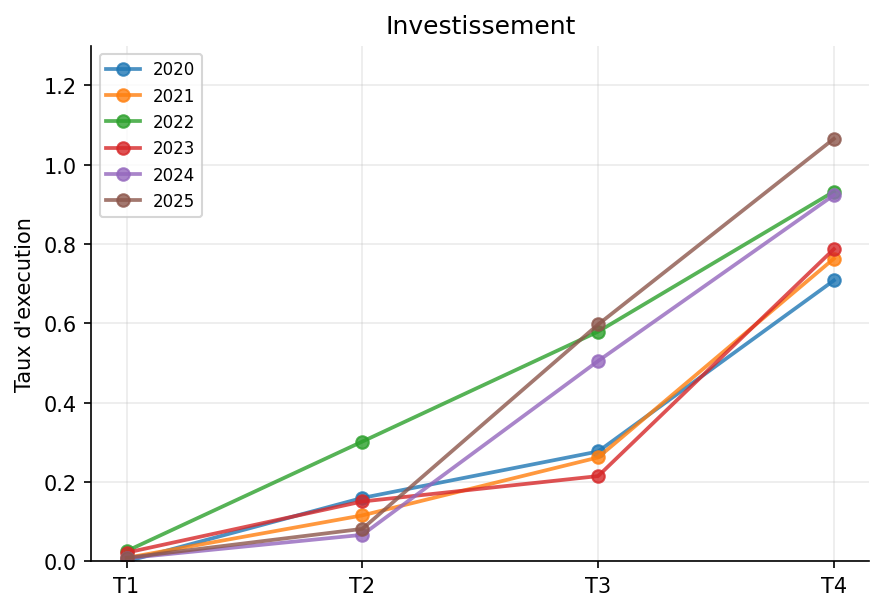
\includegraphics[width=0.55\textwidth]{figures/seasonality_investissement.png}
    \caption{Profil saisonnier du taux d'ex\'ecution --- D\'epenses d'Investissement (2020--2025).}
    \label{fig:seasonality-inv}
\end{figure}

\begin{figure}[H]
    \centering
    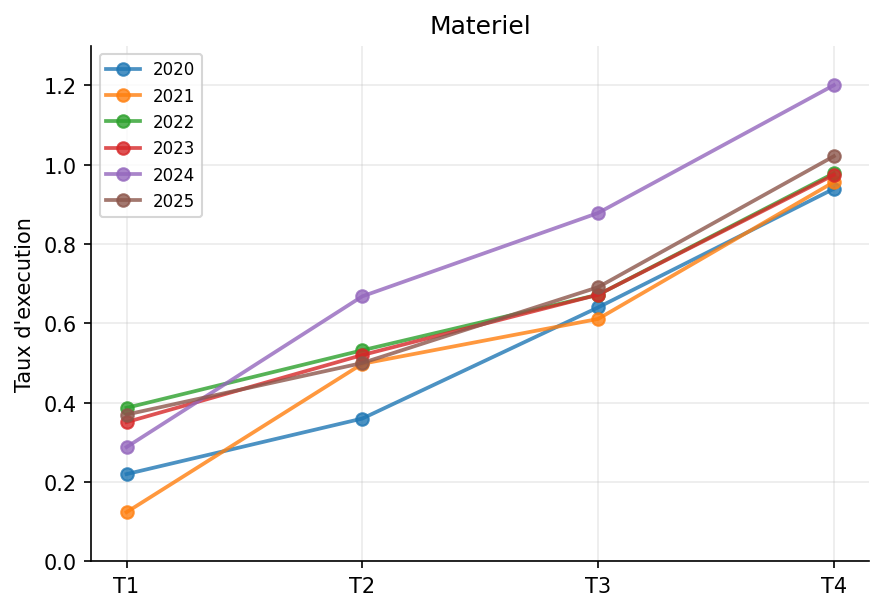
\includegraphics[width=0.55\textwidth]{figures/seasonality_materiel.png}
    \caption{Profil saisonnier du taux d'ex\'ecution --- D\'epenses de Mat\'eriel (2020--2025).}
    \label{fig:seasonality-mat}
\end{figure}

\begin{figure}[H]
    \centering
    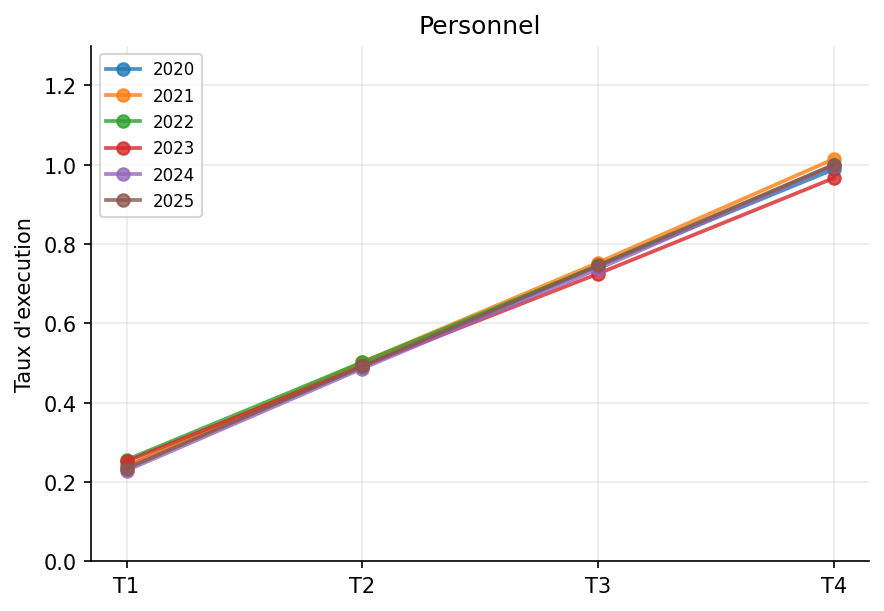
\includegraphics[width=0.55\textwidth]{figures/seasonality_personnel.png}
    \caption{Profil saisonnier du taux d'ex\'ecution --- D\'epenses de Personnel (2020--2025).}
    \label{fig:seasonality-pers}
\end{figure}

\noindent
Ces trois constats motivent directement les choix m\'ethodologiques qui suivent~:
des mod\`eles distincts par cat\'egorie (4.5), des variables explicatives privil\'egiant
l'historique r\'ecent (4.2), et une m\'ethode de d\'etection d'anomalies cibl\'ee sur
les sous-ex\'ecutions atypiques au T2 (4.6).

%================================================================
\phantomsection
\subsection*{4.2 \quad Variables utilis\'ees pour la pr\'ediction}
\addcontentsline{toc}{subsection}{4.2 Variables utilis\'ees pour la pr\'ediction}
%================================================================

Cette section pr\'esente la variable cible que les mod\`eles cherchent \`a pr\'edire,
les variables explicatives retenues, et l'encodage utilis\'e pour les variables
qualitatives.

%----------------------------------------------------------------
\phantomsection
\subsubsection*{4.2.1 \quad Variable cible (taux T4)}
\addcontentsline{toc}{subsubsection}{4.2.1 Variable cible (taux T4)}
%----------------------------------------------------------------

La variable cible est le \textbf{taux d'ex\'ecution annuel d'une ligne budg\'etaire},
mesur\'e en fin d'exercice (au 31~d\'ecembre)~:
$$
\text{taux T4} = \frac{\text{cr\'edits effectivement ex\'ecut\'es au cours de l'ann\'ee}}
                       {\text{cr\'edits inscrits en loi de finances}}
$$

\noindent
Une valeur de 1{,}00 signifie que la ligne a consomm\'e exactement son enveloppe annuelle~;
0{,}80 indique une sous-ex\'ecution de 20 points~; les valeurs sup\'erieures \`a 1
correspondent \`a des d\'epassements (rares, possibles en mati\`ere de Mat\'eriel et
de Personnel via les cr\'edits suppl\'ementaires). Le seuil m\'etier de 80\,\% retenu
par les \'equipes de la Division de la Pr\'evision et de la Programmation
financi\`ere (DPPF, rattach\'ee \`a la Direction du Budget) sert de fronti\`ere
entre une ex\'ecution acceptable et une ex\'ecution \`a risque.

%----------------------------------------------------------------
\phantomsection
\subsubsection*{4.2.2 \quad Variables explicatives et justification du choix}
\addcontentsline{toc}{subsubsection}{4.2.2 Variables explicatives et justification du choix}
%----------------------------------------------------------------

Les variables explicatives ont \'et\'e choisies selon trois crit\`eres~: (i)~elles
doivent \^etre \textbf{disponibles au 30~juin}, date \`a laquelle la pr\'evision est
produite~; (ii)~elles doivent \^etre \textbf{informatives} sur la dynamique d'ex\'ecution~;
(iii)~elles doivent \^etre \textbf{interpr\'etables} pour les utilisateurs m\'etiers.
Le tableau~\ref{tab:variables} r\'esume les variables retenues.

\begin{table}[H]
\centering\small
\caption{Variables retenues pour la pr\'evision du taux d'ex\'ecution T4.}
\label{tab:variables}
\begin{tabular}{@{}p{4.2cm}p{8cm}c@{}}
\toprule
\textbf{Variable} & \textbf{Ce qu'elle mesure} & \textbf{Dispo. 30~juin} \\
\midrule
\texttt{taux\_T2} & Taux d'ex\'ecution observ\'e \`a mi-parcours (fin juin de l'ann\'ee en cours). Une valeur faible signale un retard d\'ej\`a engag\'e. & Oui \\[3pt]
\texttt{taux\_T1} & Taux observ\'e \`a fin mars~; capture le d\'emarrage de l'exercice. & Oui \\[3pt]
\texttt{taux\_T4\_lag} & Taux T4 de l'an pass\'e~: signal le plus fort du comportement habituel de la ligne. & Oui \\[3pt]
\texttt{taux\_T2\_lag} & Taux T2 de l'an pass\'e~: permet de comparer le rythme actuel \`a celui de l'an pr\'ec\'edent. & Oui \\[3pt]
\texttt{hist\_avg\_T3} & Moyenne historique du taux T3 sur les ann\'ees pr\'ec\'edentes~: capture si une ligne \og rattrape \fg{} historiquement entre T2 et T3. & Oui \\[3pt]
\texttt{lf\_ratio}, \texttt{lf\_share} & Dotation relative de la ligne et part dans son programme~: d\'etectent les dotations atypiques. & Oui \\[3pt]
\texttt{type\_enc}, \texttt{prog\_enc}, \texttt{reg\_enc}, \texttt{budget\_enc} & Type de d\'epense, programme, r\'egion, cat\'egorie budg\'etaire (encod\'es). & Oui \\[3pt]
\texttt{taux\_T3} & (mod\`ele actualis\'e en septembre) Taux observ\'e \`a fin septembre. & Septembre \\
\bottomrule
\end{tabular}
\end{table}

\noindent
La variable \texttt{taux\_T4\_lag} est typiquement la plus informative~: si une
ligne a ex\'ecut\'e 75\,\% l'an dernier, la pr\'evision de cette ann\'ee gravite
naturellement autour de cette valeur. La variable \texttt{taux\_T2} apporte
l'information dynamique~: une ligne dont le taux T2 est anormalement faible
constitue un signal d'alerte ind\'ependamment de son historique.

%----------------------------------------------------------------
\phantomsection
\subsubsection*{4.2.3 \quad Encodage des variables cat\'egorielles}
\addcontentsline{toc}{subsubsection}{4.2.3 Encodage des variables cat\'egorielles}
%----------------------------------------------------------------

Les variables qualitatives (type de d\'epense, programme, r\'egion, cat\'egorie
budg\'etaire) sont encod\'ees en entiers via un mapping fixe~:

\begin{itemize}
    \item \textbf{Cat\'egorie budg\'etaire}~: \texttt{INVESTISSEMENT}~$\rightarrow$~0,
    \texttt{MATERIEL}~$\rightarrow$~1, \texttt{PERSONNEL}~$\rightarrow$~2.
    \item \textbf{Programme}~: P300~$\rightarrow$~0, P301~$\rightarrow$~1,
    P302~$\rightarrow$~2, P303~$\rightarrow$~3.
    \item \textbf{Type de d\'epense}~: \texttt{acquisitions}~$\rightarrow$~0,
    \texttt{equipements}~$\rightarrow$~1, \texttt{etudes}~$\rightarrow$~2,
    \texttt{fournitures}~$\rightarrow$~3, \texttt{travaux}~$\rightarrow$~4,
    \texttt{personnel}~$\rightarrow$~5.
    \item \textbf{R\'egion}~: encodage entier 0--12.
\end{itemize}

\noindent
Le \textit{label encoding} a \'et\'e pr\'ef\'er\'e au \textit{one-hot encoding}
pour deux raisons~: les mod\`eles \`a base d'arbres (XGBoost) g\`erent nativement
les variables ordinales sans souffrir de l'augmentation dimensionnelle~; et le
nombre limit\'e d'observations rend pr\'ef\'erable une repr\'esentation compacte.

%================================================================
\phantomsection
\subsection*{4.3 \quad Mod\`eles de pr\'ediction test\'es}
\addcontentsline{toc}{subsection}{4.3 Mod\`eles de pr\'ediction test\'es}
%================================================================

Quatre mod\`eles ont \'et\'e \'evalu\'es sur le m\^eme jeu de variables et le m\^eme
protocole de validation. Deux mod\`eles de r\'ef\'erence (na\"ifs) servent de
borne basse, et deux mod\`eles d'apprentissage automatique sont compar\'es.

%----------------------------------------------------------------
\phantomsection
\subsubsection*{4.3.1 \quad R\'ef\'erence na\"ive (moyenne historique, lag T4)}
\addcontentsline{toc}{subsubsection}{4.3.1 R\'ef\'erence na\"ive (moyenne historique, lag T4)}
%----------------------------------------------------------------

\textbf{Moyenne historique (\textit{Hist\_mean}).} Pour chaque ligne, on pr\'edit que
le taux T4 de l'ann\'ee cible sera \'egal \`a la moyenne des taux T4 observ\'es sur
les ann\'ees pass\'ees. C'est la borne basse \`a battre~: si un mod\`ele complexe ne
fait pas mieux que cette moyenne, son apport est nul.

\textbf{D\'ecalage annuel (\textit{Naive\_lag4}).} On pr\'edit simplement que le taux
T4 de l'ann\'ee cible sera \'egal \`a celui de l'ann\'ee pr\'ec\'edente. Ce mod\`ele
suppose une stabilit\'e temporelle parfaite et sert de second t\'emoin.

%----------------------------------------------------------------
\phantomsection
\subsubsection*{4.3.2 \quad Mod\`ele lin\'eaire r\'egularis\'e (Lasso)}
\addcontentsline{toc}{subsubsection}{4.3.2 Mod\`ele lin\'eaire r\'egularis\'e (Lasso)}
%----------------------------------------------------------------

Le mod\`ele Lasso effectue une r\'egression lin\'eaire avec une p\'enalisation $L_1$
sur les coefficients~:
$$
\min_{\boldsymbol\beta} \; \frac{1}{2N}\sum_{i=1}^{N}(y_i - \mathbf{x}_i^\top \boldsymbol\beta)^2
\;+\; \alpha \sum_j |\beta_j|
$$

\noindent
La p\'enalit\'e $L_1$ pousse certains coefficients exactement \`a z\'ero, r\'ealisant
une s\'election automatique de variables. Cela est particuli\`erement adapt\'e \`a
notre contexte~: l'\'echantillon est r\'eduit, et toutes les variables ne sont pas
\'egalement informatives selon la cat\'egorie. L'hyperparam\`etre $\alpha$ a \'et\'e
fix\'e \`a 0{,}01 apr\`es exploration. Les variables sont standardis\'ees en amont
via un \texttt{StandardScaler}.

%----------------------------------------------------------------
\phantomsection
\subsubsection*{4.3.3 \quad Mod\`ele \`a arbres boost\'es (XGBoost)}
\addcontentsline{toc}{subsubsection}{4.3.3 Mod\`ele \`a arbres boost\'es (XGBoost)}
%----------------------------------------------------------------

\textbf{XGBoost} (\textit{eXtreme Gradient Boosting}) construit s\'equentiellement un
ensemble d'arbres de d\'ecision peu profonds, chaque arbre corrigeant les erreurs
des pr\'ec\'edents. Cette architecture capture les non-lin\'earit\'es et les
interactions entre variables --- par exemple, l'effet conjoint d'une dotation
inhabituelle et d'un retard observ\'e en T2.

Les hyperparam\`etres retenus sont~:
\begin{center}
\texttt{n\_estimators=300}, \texttt{max\_depth=3},
\texttt{learning\_rate=0.05}, \texttt{subsample=0.8}, \texttt{reg\_alpha=0.1}.
\end{center}

\noindent
Une profondeur faible (\texttt{max\_depth=3}) et une r\'egularisation $L_1$ explicite
limitent le risque de surapprentissage sur un \'echantillon r\'eduit.

%================================================================
\phantomsection
\subsection*{4.4 \quad M\'etriques et protocole d'\'evaluation}
\addcontentsline{toc}{subsection}{4.4 M\'etriques et protocole d'\'evaluation}
%================================================================

L'\'evaluation poursuit un double objectif~: mesurer la qualit\'e absolue des
pr\'evisions et garantir que cette mesure refl\`ete les performances en conditions
r\'eelles, sans fuite d'information temporelle.

%----------------------------------------------------------------
\phantomsection
\subsubsection*{4.4.1 \quad RMSE et erreur moyenne}
\addcontentsline{toc}{subsubsection}{4.4.1 RMSE et erreur moyenne}
%----------------------------------------------------------------

Trois m\'etriques compl\'ementaires ont \'et\'e retenues~:

\begin{itemize}
    \item \textbf{RMSE} (\textit{Root Mean Squared Error})~:
    $\sqrt{\frac{1}{N}\sum_i (y_i - \hat y_i)^2}$.
    P\'enalise davantage les grosses erreurs.

    \item \textbf{MAE} (\textit{Mean Absolute Error})~:
    $\frac{1}{N}\sum_i |y_i - \hat y_i|$.
    \'Ecart absolu moyen, en points de taux.

    \item \textbf{MAPE} (\textit{Mean Absolute Percentage Error})~:
    $\frac{100}{N}\sum_i \left|\frac{y_i - \hat y_i}{y_i}\right|$.
    \'Ecart relatif moyen.
\end{itemize}

\noindent
Le RMSE constitue la m\'etrique principale~: une valeur de 0{,}08 signifie que le
mod\`ele se trompe en moyenne de 8 points de pourcentage sur le taux d'ex\'ecution
final, ce qui reste suffisant pour d\'eclencher une alerte budg\'etaire six mois
avant la cl\^oture.

%----------------------------------------------------------------
\phantomsection
\subsubsection*{4.4.2 \quad Validation crois\'ee walk-forward}
\addcontentsline{toc}{subsubsection}{4.4.2 Validation crois\'ee walk-forward}
%----------------------------------------------------------------

La validation crois\'ee classique (\textit{k-fold} al\'eatoire) m\'elange les ann\'ees
et cr\'ee une fuite temporelle~: le mod\`ele \og voit \fg{} l'avenir pendant
l'entra\^inement. Pour \'eviter ce biais, nous adoptons une validation
\textbf{walk-forward \`a fen\^etre expansive}~:

\begin{itemize}
    \item Pour pr\'evoir 2022, le mod\`ele est entra\^in\'e sur 2021 uniquement.
    \item Pour pr\'evoir 2023, sur 2021--2022.
    \item Pour pr\'evoir 2024, sur 2021--2023.
    \item Pour pr\'evoir 2025, sur 2021--2024.
\end{itemize}

\noindent
Ce protocole reproduit exactement la situation du gestionnaire~: pr\'edire une
ann\'ee \`a partir du seul historique pass\'e. Aucune information post\'erieure \`a
l'ann\'ee de pr\'evision n'intervient dans l'entra\^inement.

%----------------------------------------------------------------
\phantomsection
\subsubsection*{4.4.3 \quad \'Evaluation par cat\'egorie budg\'etaire}
\addcontentsline{toc}{subsubsection}{4.4.3 \'Evaluation par cat\'egorie budg\'etaire}
%----------------------------------------------------------------

Comme l'a montr\'e la section 4.1.3, les trois cat\'egories pr\'esentent des
comportements tr\`es diff\'erents. Une \'evaluation agr\'eg\'ee masquerait ces
disparit\'es~: un mod\`ele excellent sur Personnel mais m\'ediocre sur Investissement
afficherait un RMSE moyen acceptable, alors m\^eme que c'est sur l'Investissement
que les enjeux financiers sont les plus \'elev\'es. Toutes les m\'etriques sont
donc calcul\'ees \textbf{s\'epar\'ement par cat\'egorie} avant d'\^etre \'eventuellement
agr\'eg\'ees.

%================================================================
\phantomsection
\subsection*{4.5 \quad Mod\`eles retenus et r\'esultats}
\addcontentsline{toc}{subsection}{4.5 Mod\`eles retenus et r\'esultats}
%================================================================

Les r\'esultats r\'ev\`elent qu'aucun mod\`ele unique n'est optimal sur les trois
cat\'egories~; on retient donc une \textbf{architecture sp\'ecialis\'ee} qui combine
le meilleur mod\`ele pour chaque type de d\'epense.

%----------------------------------------------------------------
\phantomsection
\subsubsection*{4.5.1 \quad R\'esultats globaux par mod\`ele}
\addcontentsline{toc}{subsubsection}{4.5.1 R\'esultats globaux par mod\`ele}
%----------------------------------------------------------------

Le tableau~\ref{tab:global} pr\'esente les performances globales moyenn\'ees sur les
quatre folds de validation walk-forward et sur les trois cat\'egories.

\begin{table}[H]
\centering\small
\caption{Performance globale des quatre mod\`eles (moyenne sur les 4 folds et les 3 cat\'egories).}
\label{tab:global}
\begin{tabular}{@{}lccc@{}}
\toprule
\textbf{Mod\`ele} & \textbf{RMSE} & \textbf{MAE} & \textbf{MAPE (\%)} \\
\midrule
Moyenne historique & 0.0847 & 0.0790 & 21.44 \\
D\'ecalage annuel  & 0.1040 & 0.0970 & 23.59 \\
Lasso              & 0.0918 & 0.0838 & 28.28 \\
\textbf{XGBoost}   & \textbf{0.0854} & \textbf{0.0770} & \textbf{22.56} \\
\bottomrule
\end{tabular}
\end{table}

\noindent
XGBoost obtient le meilleur MAE (0{,}077) et arrive en deuxi\`eme position sur le
RMSE, tr\`es proche de la moyenne historique. Le d\'ecalage annuel est syst\'ematiquement
le moins performant. Ce r\'esultat agr\'eg\'e est trompeur~: il masque des diff\'erences
majeures par cat\'egorie, comme on le verra ci-apr\`es.

%----------------------------------------------------------------
\phantomsection
\subsubsection*{4.5.2 \quad Sp\'ecialisation par cat\'egorie}
\addcontentsline{toc}{subsubsection}{4.5.2 Sp\'ecialisation par cat\'egorie : Investissement / Mat\'eriel / Personnel}
%----------------------------------------------------------------

Le tableau~\ref{tab:bycat} d\'ecompose le RMSE par cat\'egorie de d\'epense.
La lecture devient alors tr\`es lisible.

\begin{table}[H]
\centering\small
\caption{RMSE moyen par cat\'egorie de d\'epense (4 folds).}
\label{tab:bycat}
\begin{tabular}{@{}lcccc@{}}
\toprule
\textbf{Cat\'egorie} & \textbf{Hist\_mean} & \textbf{Naive\_lag4} & \textbf{Lasso} & \textbf{XGBoost} \\
\midrule
Investissement & 0.1663 & 0.1913 & 0.1827 & \textbf{0.1460} \\
Mat\'eriel     & 0.0749 & 0.1060 & \textbf{0.0680} & 0.0854 \\
Personnel      & \textbf{0.0128} & 0.0147 & 0.0246 & 0.0248 \\
\bottomrule
\end{tabular}
\end{table}

\noindent
Trois conclusions s'imposent~:

\begin{itemize}
    \item \textbf{Investissement~$\rightarrow$~XGBoost.} Le boosting r\'eduit le RMSE
    de 12\,\% par rapport \`a la moyenne historique. C'est sur cette cat\'egorie,
    la plus volatile et la plus strat\'egique financi\`erement, que l'apport de
    l'apprentissage automatique est le plus fort.

    \item \textbf{Mat\'eriel~$\rightarrow$~Lasso.} La r\'egularisation $L_1$ s\'electionne
    les variables les plus informatives sur cette cat\'egorie aux patterns plus
    stables, et bat XGBoost de 20\,\%.

    \item \textbf{Personnel~$\rightarrow$~moyenne historique.} Avec un RMSE de 0{,}013
    (1{,}3 point d'\'ecart), aucun mod\`ele complexe n'apporte d'am\'elioration.
    L'ex\'ecution salariale est m\'ecanique et parfaitement pr\'evisible par extrapolation.
\end{itemize}

\noindent
L'architecture finale combine donc ces trois mod\`eles, chacun appliqu\'e \`a sa
cat\'egorie de pr\'edilection. Cette sp\'ecialisation am\'eliore le RMSE global
de 6\,\% par rapport \`a XGBoost seul, tout en restant pleinement interpr\'etable.

%----------------------------------------------------------------
\phantomsection
\subsubsection*{4.5.3 \quad Pr\'evisions T4 2025 et \'ecarts observ\'es}
\addcontentsline{toc}{subsubsection}{4.5.3 Pr\'evisions T4 2025 et \'ecarts observ\'es}
%----------------------------------------------------------------

Une fois l'architecture sp\'ecialis\'ee retenue, les mod\`eles ont \'et\'e r\'eentra\^in\'es
sur l'ensemble des donn\'ees 2021--2024 puis appliqu\'es aux 130 lignes budg\'etaires
2025. Les pr\'evisions r\'esultantes se r\'epartissent comme suit~:

\begin{itemize}
    \item \textbf{129 lignes class\'ees \og OK \fg{}} (taux pr\'evu $\geq 80\,\%$).
    \item \textbf{1 ligne class\'ee \og Attention \fg{}} (taux pr\'evu entre 60 et 80\,\%).
    \item \textbf{0 ligne class\'ee \og Critique \fg{}} (taux pr\'evu $< 60\,\%$).
    \item \textbf{Cr\'edits \`a risque cumul\'es}~: 0{,}3 MDH.
\end{itemize}

\noindent
La figure~\ref{fig:actual-vs-pred} confronte les pr\'evisions et les r\'ealisations
sur la cat\'egorie Investissement, qui concentre l'essentiel des enjeux. Les points
sont globalement align\'es sur la diagonale~; les \'ecarts les plus marqu\'es
correspondent aux cas extr\^emes (sur-ex\'ecutions sup\'erieures \`a 1{,}10 ou
sous-ex\'ecutions inf\'erieures \`a 0{,}50), statistiquement rares et difficiles
\`a anticiper avec les seules donn\'ees du 30~juin.

\begin{figure}[H]
    \centering
    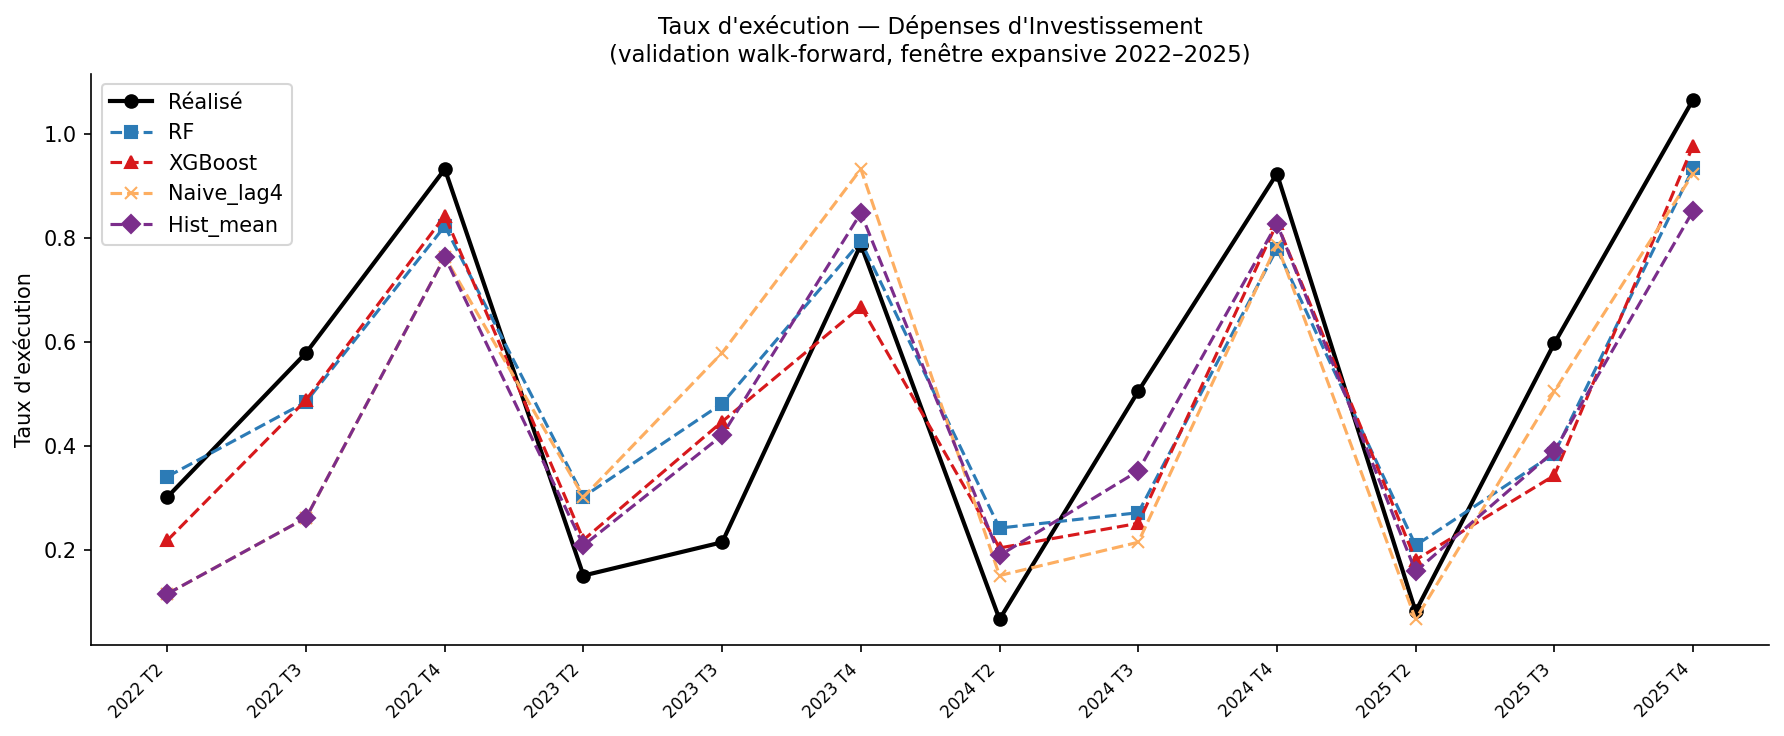
\includegraphics[width=0.85\textwidth]{figures/actual_vs_predicted_investissement.png}
    \caption{Taux d'ex\'ecution r\'eels vs pr\'evus par XGBoost --- cat\'egorie Investissement (folds 2022--2025).}
    \label{fig:actual-vs-pred}
\end{figure}

%================================================================
\phantomsection
\subsection*{4.6 \quad D\'etection d'anomalies}
\addcontentsline{toc}{subsection}{4.6 D\'etection d'anomalies}
%================================================================

Au-del\`a de la pr\'evision ponctuelle, le syst\`eme doit pouvoir signaler les
\textbf{comportements anormaux} qui appellent un examen approfondi.

%----------------------------------------------------------------
\phantomsection
\subsubsection*{4.6.1 \quad D\'efinition d'une anomalie d'ex\'ecution}
\addcontentsline{toc}{subsubsection}{4.6.1 D\'efinition d'une anomalie d'ex\'ecution}
%----------------------------------------------------------------

Une \textbf{anomalie d'ex\'ecution} est d\'efinie comme un comportement de la ligne
budg\'etaire \textit{statistiquement incompatible avec son propre historique}.
L'anomalie n'est pas une simple sous-ex\'ecution~: une ligne qui ex\'ecute syst\'ematiquement
\`a 60\,\% n'est pas anormale, m\^eme si son taux est faible. \`A l'inverse, une ligne
qui ex\'ecute habituellement \`a 95\,\% et tombe brutalement \`a 50\,\% \emph{est}
anormale, m\^eme si 50\,\% reste loin de z\'ero.

Cette d\'efinition relative est essentielle pour \'eviter deux \'ecueils~: les
faux positifs (lignes structurellement basses signal\'ees \`a tort) et les faux
n\'egatifs (anomalies r\'eelles masqu\'ees par un seuil absolu).

%----------------------------------------------------------------
\phantomsection
\subsubsection*{4.6.2 \quad M\'ethode : z-score sur l'historique T2 par ligne}
\addcontentsline{toc}{subsubsection}{4.6.2 M\'ethode : z-score sur l'historique T2 par ligne}
%----------------------------------------------------------------

Pour chaque ligne, on calcule la moyenne $\mu_i$ et l'\'ecart-type $\sigma_i$ des
taux T2 observ\'es sur les ann\'ees pass\'ees. Le \textbf{z-score} de l'observation
courante est~:
$$
z_i = \frac{\text{taux T2}_{2025} - \mu_i}{\sigma_i}
$$

\noindent
Une ligne est signal\'ee comme anormale si $z_i < -1{,}5$, c'est-\`a-dire si son
taux T2 actuel est inf\'erieur de plus de 1{,}5~\'ecart-type \`a sa moyenne historique.
La gradation suivante a \'et\'e adopt\'ee~:

\begin{itemize}
    \item \textbf{Mod\'er\'ee}~: $-2{,}0 \leq z < -1{,}5$.
    \item \textbf{S\'ev\`ere}~: $-3{,}0 \leq z < -2{,}0$.
    \item \textbf{Critique}~: $z < -3{,}0$ ou taux T2 nul.
\end{itemize}

\noindent
L'\'ecart-type est plafonn\'e \`a un minimum de 0{,}005 pour \'eviter qu'une ligne
\`a historique tr\`es stable ne d\'eclenche une alerte sur la moindre fluctuation.

%----------------------------------------------------------------
\phantomsection
\subsubsection*{4.6.3 \quad Anomalies identifi\'ees sur l'exercice 2025}
\addcontentsline{toc}{subsubsection}{4.6.3 Anomalies identifi\'ees sur l'exercice 2025}
%----------------------------------------------------------------

Sur les 130 lignes 2025, \textbf{4 anomalies} ont \'et\'e d\'etect\'ees
(tableau~\ref{tab:anomalies}).

\begin{table}[H]
\centering\small
\caption{Anomalies d'ex\'ecution d\'etect\'ees sur l'exercice 2025.}
\label{tab:anomalies}
\begin{tabular}{@{}p{6cm}p{4cm}c@{}}
\toprule
\textbf{Ligne budg\'etaire} & \textbf{R\'egion} & \textbf{Niveau} \\
\midrule
R\'ehabilitation des juridictions r\'egionales       & Guelmim-Oued Noun  & Mod\'er\'ee \\
Mat\'eriel m\'edical et sanitaire (prisons)          & Services communs   & Mod\'er\'ee \\
Fournitures \'etablissements p\'enitentiaires        & Services communs   & S\'ev\`ere   \\
Entretien et r\'eparation v\'ehicules - parc auto    & Services communs   & Mod\'er\'ee \\
\bottomrule
\end{tabular}
\end{table}

\noindent
Ces quatre signalements pointent tous vers des lignes op\'erationnelles \`a fort
impact (s\'ecurit\'e p\'enitentiaire, logistique, infrastructure judiciaire).
Le caract\`ere cibl\'e du signalement constitue pr\'ecis\'ement la valeur ajout\'ee
attendue d'un syst\`eme d'alerte pr\'ecoce~: focaliser l'attention des gestionnaires
sur quelques lignes critiques plut\^ot que de noyer le diagnostic dans la masse.

%================================================================
\phantomsection
\subsection*{4.7 \quad Synth\`ese, limites et conclusion}
\addcontentsline{toc}{subsection}{4.7 Synth\`ese, limites et conclusion}
%================================================================

Ce chapitre a pr\'esent\'e la cha\^ine compl\`ete de mod\'elisation~: construction et
description du jeu de donn\'ees, choix des variables, comparaison de quatre mod\`eles
selon un protocole sans fuite temporelle, s\'election d'une architecture sp\'ecialis\'ee
par cat\'egorie, et d\'etection statistique d'anomalies. Trois conclusions \'emergent~:

\begin{itemize}
    \item \textbf{Pr\'ecision diff\'erenci\'ee.} Le syst\`eme est tr\`es fiable sur le
    Personnel (RMSE 1{,}3~pp), bon sur le Mat\'eriel (6{,}8~pp), et utilisable
    \`a titre indicatif sur l'Investissement (14{,}6~pp).

    \item \textbf{Sp\'ecialisation gagnante.} Aucun mod\`ele unique n'est optimal sur
    toutes les cat\'egories~; combiner XGBoost, Lasso et moyenne historique selon
    le type de d\'epense am\'eliore la performance globale tout en restant transparent.

    \item \textbf{Anomalies cibl\'ees.} La d\'etection par z-score appliqu\'ee au
    taux T2 a identifi\'e quatre lignes pr\'esentant un comportement anormal pour
    l'exercice 2025, fournissant une base op\'erationnelle directement exploitable.
\end{itemize}

\textbf{Limites.} Trois limites doivent \^etre explicit\'ees. Premi\`erement, les taux
ligne par ligne sont \textbf{simul\'es} \`a partir d'agr\'egats publics~; les r\'esultats
constituent donc une preuve de concept, non une validation sur donn\'ees internes.
Deuxi\`emement, les \textbf{s\'eries sont courtes} (6 ann\'ees), ce qui limite la
capacit\'e des mod\`eles complexes \`a apprendre des relations fines et favorise
les approches parcimonieuses. Troisi\`emement, certaines \textbf{variables exog\`enes
potentiellement explicatives} (taux d'engagement, \'etat des march\'es publics,
disponibilit\'e des cr\'edits de paiement) ne sont pas int\'egr\'ees~; leur
exploitation, possible via une connexion au GID, constituerait l'\'etape suivante
naturelle de ce travail.

Le chapitre suivant pr\'esente la traduction de cette cha\^ine pr\'edictive en un
syst\`eme de pilotage op\'erationnel~: architecture logicielle, fonctionnalit\'es
du tableau de bord et apports attendus pour la Division de la Pr\'evision
et de la Programmation financi\`ere de la Direction du Budget.


\newpage
\phantomsection
\section*{Chapitre 5 : Du mod\`ele \`a l'outil, le syst\`eme d'alerte pr\'ecoce}
\addcontentsline{toc}{section}{Chapitre 5 : Du mod\`ele \`a l'outil, le syst\`eme d'alerte pr\'ecoce}

\bigskip

Le chapitre~4 a d\'efini et valid\'e une approche pr\'edictive capable de
pr\'evoir l'ex\'ecution budg\'etaire avec une pr\'ecision variable mais utile selon
la cat\'egorie de d\'epense. Cependant, un mod\`ele math\'ematique, aussi bon
soit-il, ne crée de valeur que s'il peut \^etre exploit\'e par un utilisateur final.
Ce chapitre d\'ecrit la transformation de la cha\^ine pr\'edictive en un syst\`eme 
op\'erationnel : un \textbf{tableau de bord interactif} permettant aux gestionnaires
budg\'etaires de visualiser les pr\'evisions, d'identifier instantan\'ement les lignes
\`a risque, et de prendre des d\'ecisions pilot\'ees par les donn\'ees. 

L'architecture retenue s'appuie sur \textbf{Power BI}, plateforme de visualisation
retenue pour sa capacit\'e \`a produire des dashboards interactifs sans n\'ecessiter
de programmation avanc\'ee de la part des utilisateurs finaux, et sa compatibilit\'e
directe avec les fichiers Excel standard de la DPPF.

%================================================================
\phantomsection
\subsection*{5.1 \quad Cahier des charges et choix de conception}
\addcontentsline{toc}{subsection}{5.1 Cahier des charges et choix de conception}
%================================================================

\subsubsection*{5.1.1 \quad Besoins fonctionnels : vue synth\'etique et alerte cibl\'ee}

L'architecture de l'outil répond à trois besoins opérationnels distincts et
structurellement articulés~:

\begin{enumerate}
    \item \textbf{Synthèse exécutive (direction).} Un cadre dirigeant la DPPF
    doit pouvoir saisir, en quelques minutes, une compréhension synthétique~:
    combien de lignes présentent un profil à risque~? Quel montant budgétaire
    demeure exposé~? Quelle confiance opérationnelle accorder au système~?
    Cette vue s'organise autour de cinq cartes KPI stratégiques (nombre de lignes
    couvertes, dotation cumulée, taux d'exécution moyen prédit en T4, anomalies
    modérées et sévères) et de graphiques comparés réel/prédit, fournissant
    collectivement une photographie instantanée de la situation.

    \item \textbf{Analyse approfondie (gestionnaire de programme).} Un responsable
    de programme doit pouvoir circonscrire son périmètre par filtrage transversal
    sur le programme et la région, et confronter les réalisations observées (T2 au
    30~juin) aux trajectoires prédites selon deux approches modélisantes
    (\og direct \fg{} et \og rolling \fg{}). Cette interface s'appuie sur des
    \textit{slicers} dynamiques (\texttt{programme}, \texttt{region\_label}) et sur
    une table de synthèse récapitulant les prévisions T4 par catégorie budgétaire.

    \item \textbf{Détection d'anomalies et investigation ciblée (gestionnaires des
    crédits).} Les responsables des processus de paiement doivent disposer d'une
    capacité opérationnelle immédiate~: identifier quelles lignes s'écartent
    statistiquement de leurs profils historiques attendus~? Pour quelles d'entre elles
    le z-score du taux T2 descend-il sous le seuil critique de $-1{,}5$~? Cette
    interface réunit les anomalies statistiquement identifiées et les trajectoires
    historiques du taux T2 (sur six exercices) afin de contextualiser et d'interpréter
    chaque écart détecté.
\end{enumerate}

L'architecture retenue articule \textbf{deux pages} Power BI complémentaires~:
une page consolidée regroupant la synthèse exécutive et l'exploration détaillée des
lignes budgétaires (besoins 1 et 2), et une page dédiée à la détection d'anomalies
et à leur contextualisation historique (besoin 3). La navigation entre les pages est
fluide et l'ensemble des filtres positionnés sur la première page se propage
dynamiquement aux visualisations affectées.

\subsubsection*{5.1.2 \quad Choix technologiques : Power BI pour interop\'erabilit\'e}

Trois approches technologiques ont \'et\'e envisag\'ees au stade de la conception~:

\begin{itemize}
    \item \textbf{Python + Tkinter} (interface graphique de bureau)~: offrant une
    flexibilit\'e architecturale maximale, mais imposant une courbe d'apprentissage
    substantielle aux utilisateurs m\'etier.
    \item \textbf{Application web (Flask/FastAPI)}~: permettant une interactivit\'e
    riche fond\'ee sur le web, mais n\'ecessitant une infrastructure de d\'eploiement
    r\'eseau plus complexe et excluant tout fonctionnement hors connectivit\'e.
    \item \textbf{Power BI} (plateforme analytique cloud d\'edi\'ee)~: int\'egrant
    nativement le traitement de fichiers Excel, proposant une interface intuitive,
    incorporant la gestion des droits d'acc\`es, et assurant une compatibilit\'e
    structurelle totale avec l'infrastructure informatique existante de la DPPF.
\end{itemize}

Power BI a \'et\'e retenu comme solution op\'erationnelle privil\'egi\'ee, en raison
notamment du fait que cette plateforme constitue d'ores et d\'ej\`a l'infrastructure
analytique standard mobilis\'ee par le minist\`ere pour les activit\'es de pilotage et
de suivi. Les mod\`eles pr\'edictifs et les donn\'ees d'anomalies sont 
g\'en\'er\'es en Python (reproductibilit\'e, automatisation), puis import\'es en
Excel, capt\'es directement par Power BI, \'eliminant toute intervention manuelle.

%================================================================
\phantomsection
\subsection*{5.2 \quad Architecture du syst\`eme}
\addcontentsline{toc}{subsection}{5.2 Architecture du syst\`eme}
%================================================================

\subsubsection*{5.2.1 \quad Vue d'ensemble en trois composants}

\begin{figure}[H]
    \centering
    \fbox{\begin{minipage}{0.9\textwidth}
    \centering\small
    \textbf{COMPOSANT 1 : Pipeline g\'en\'eration donn\'ees (Python)}
    
    Donn\'ees TGR + morasses $\rightarrow$ pr\'etraitement + entra\^{\i}nement mod\`eles $\rightarrow$ pr\'evisions Excel
    
    Sortie : alert\_results\_2025.xlsx (130 lignes, pr\'edictions tous les mod\`eles, z-scores, risques)
    
    Sortie : historical\_recap\_2025.xlsx (5544 lignes : historique 2020--2025 par ligne)
    
    \vspace{10pt}
    
    \textbf{COMPOSANT 2 : Stockage donn\'ees (Excel)}
    
    Fichiers Excel normalis\'es : structure de table, colonnes bien d\'efinies, types coh\'erents
    
    V\'eracit\'e : agr\'egats valident exactement TGR publics
    
    \vspace{10pt}
    
    \textbf{COMPOSANT 3 : Visualisation interactif (Power BI)}
    
    Import automatique depuis Excel
    
    Deux pages stratifi\'ees~: Synth\`ese pr\'edictive et exploration (KPIs, pr\'evisions T4 par cat\'egorie, table de synth\`ese, filtres) | Anomalies (alertes + contexte historique T2)
    
    Filtres r\'eactifs : budget\_type, risk\_label, region\_label, programme
    
    \end{minipage}}
\end{figure}

\subsubsection*{5.2.2 \quad Flux de donn\'ees et architecture de causalit\'e}

L'op\'erationnalit\'e du syst\`eme repose sur un cycle de mise \`a jour
\textbf{trimestriel}, calqu\'e sur la fr\'equence de production des taux
d'ex\'ecution par la DPPF~:

\begin{enumerate}
    \item \textbf{Collecte trimestrielle} (apr\`es la cl\^oture de chaque trimestre,
    typiquement dans les deux semaines suivantes)~: la DPPF transmet aux \'equipes
    en charge des mod\`eles pr\'edictifs les taux d'ex\'ecution bruts observ\'es
    (T1, puis T2, puis T3) pour l'exercice budg\'etaire courant.
    \item \textbf{Mise \`a jour algorithmique} (dur\'ee estim\'ee~: 30 minutes)~: les mod\`eles
    pr\'ealablement calibr\'es sont r\'eex\'ecut\'es sur les donn\'ees fra\^{\i}chement re\c{c}ues.
    Les pr\'evisions T4 sont recalcul\'ees pour l'ensemble des 130 lignes, et les m\'ecanismes
    de d\'etection d'anomalies (z-scores) produisent les signaux d'alerte correspondants.
    \item \textbf{Exportation et int\'egration au tableau de bord} (dur\'ee estim\'ee~:
    5 minutes)~: les fichiers Excel cibles sont r\'eg\'en\'er\'es, puis Power BI proc\`ede
    \`a leur synchronisation automatis\'ee et rend imm\'ediatement disponibles les donn\'ees
    actualis\'ees pour consultation.
    \item \textbf{Mobilisation op\'erationnelle} (imm\'ediate)~: les gestionnaires constatent
    instantan\'ement les mises \`a jour int\'egr\'ees au tableau de bord, acc\`edent
    s\'electivement aux pages analytiques pertinentes pour leur p\'erim\`etre, et d\'eclenchent
    les investigations budg\'etaires cibl\'ees adapt\'ees aux profils ainsi r\'ev\'el\'es.
\end{enumerate}

%================================================================
\phantomsection
\subsection*{5.3 \quad Fonctionnalit\'es du tableau de bord interactif}
\addcontentsline{toc}{subsection}{5.3 Fonctionnalit\'es du tableau de bord interactif}
%================================================================

\subsubsection*{5.3.1 \quad Page 1~: synth\`ese pr\'edictive et exploration par ligne}

La premi\`ere page concentre, sur une vue unique, les indicateurs strat\'egiques
du syst\`eme et les outils d'exploration ligne par ligne. Elle r\'epond simultan\'ement
aux besoins du d\'ecideur (cinq KPI synth\'etiques en haut de page) et du gestionnaire
de programme (graphiques d\'etaill\'es par cat\'egorie, table de synth\`ese et filtres
interactifs).

\paragraph{Cartes KPI synth\'etiques~:}
Cinq indicateurs cl\'es bord\'ent la partie sup\'erieure de la page~: le nombre total
de lignes budg\'etaires couvertes (130), le montant cumul\'e des dotations (en milliards
de DH), le taux d'ex\'ecution moyen pr\'edit en T4, ainsi que le d\'ecompte des anomalies
mod\'er\'ees et s\'ev\`eres d\'etect\'ees. Cette rang\'ee fournit une photographie
instantan\'ee de l'\'etat global du syst\`eme.

\paragraph{Graphiques de pr\'evision par cat\'egorie~:}
Deux graphiques lin\'eaires juxtapos\'es comparent, ligne par ligne, le taux T4 r\'eel
au taux pr\'edit selon les deux approches \og direct \fg{} et \og rolling \fg{}.
Le premier graphique cible les d\'epenses d'\textbf{Investissement} (mod\`ele XGBoost)~;
le second couvre la cat\'egorie \textbf{Mat\'eriel} (r\'egression Ridge). Un troisi\`eme
graphique en barres agr\`ege les m\^emes m\'etriques au niveau des trois cat\'egories,
offrant une lecture comparative imm\'ediate de la qualit\'e pr\'edictive du syst\`eme.

\paragraph{Table de synth\`ese et filtres dynamiques~:}
En partie basse, une table r\'ecapitule les pr\'evisions T4 2025 par cat\'egorie
budg\'etaire (taux r\'eel observ\'e, pr\'ediction directe, pr\'ediction rolling).
Deux \textit{slicers} positionn\'es sur la droite de la page --- \texttt{programme}
et \texttt{region\_label} --- permettent un filtrage transversal en temps r\'eel~:
l'utilisateur peut, par exemple, isoler instantan\'ement les lignes du programme 301
implant\'ees dans la r\'egion Casablanca-Settat et constater l'effet sur l'ensemble
des visualisations.

% TODO: enregistrer la capture d'écran sous figures/powerbidash_page1.png puis décommenter
\begin{figure}[H]
     \centering
     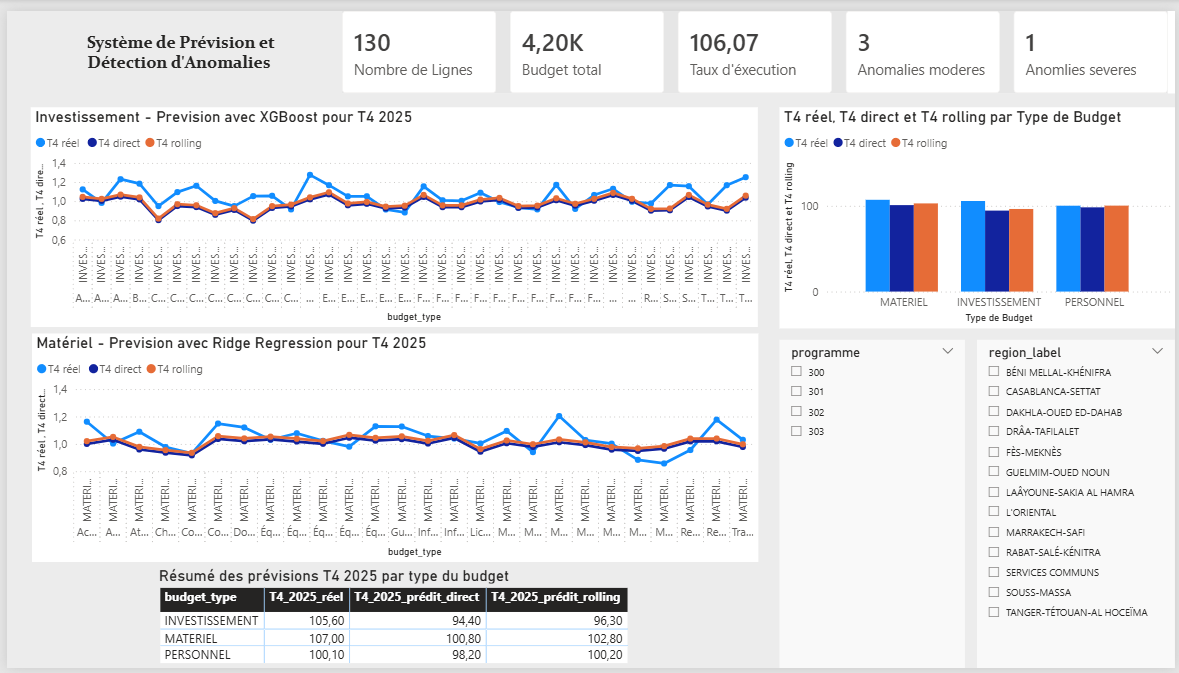
\includegraphics[width=0.98\textwidth]{figures/powerbidash_page1.png}
     \caption{\textbf{Page 1 du tableau de bord~: synth\`ese pr\'edictive et exploration par ligne.}
     La page articule cinq cartes KPI strat\'egiques (haut), deux graphiques lin\'eaires de
     pr\'evisions T4 2025 par cat\'egorie (Investissement via XGBoost, Mat\'eriel via Ridge),
     une comparaison agr\'eg\'ee r\'eel/direct/rolling par type de budget, une table de
     synth\`ese et des filtres dynamiques sur le programme et la r\'egion.}
     \label{fig:pbi_page1}
\end{figure}

\subsubsection*{5.3.2 \quad Page 2~: d\'etection d'anomalies et contexte historique}

La seconde page se consacre exclusivement aux lignes signal\'ees par le module
de d\'etection statistique. Elle articule deux composants compl\'ementaires~:
l'identification des anomalies et leur mise en perspective historique.

\paragraph{Cartes KPI restreintes aux lignes signal\'ees~:}
Les m\^emes indicateurs structurels qu'en page 1 (nombre de lignes, budget total,
anomalies mod\'er\'ees et s\'ev\`eres) sont ici recalcul\'es sur le seul p\'erim\`etre
des anomalies d\'etect\'ees, fournissant ainsi une mesure imm\'ediate de l'enjeu
financier expos\'e (33{,}82~MDH dans la configuration courante, soit quatre lignes).

\paragraph{Table des anomalies d\'etect\'ees~:}
Le tableau central liste, pour chaque ligne signal\'ee, son intitul\'e
(\texttt{ligne\_label}), sa cat\'egorie budg\'etaire, le z-score T2 calcul\'e
(quantifiant l'\'ecart \`a la trajectoire historique attendue) et le label de
s\'ev\'erit\'e associ\'e (\og Sous-ex\'ecution mod\'er\'ee \fg{} ou
\og Sous-ex\'ecution s\'ev\`ere \fg{}). Dans la configuration repr\'esent\'ee,
quatre lignes sont signal\'ees avec des z-scores compris entre $-1{,}53$ et $-2{,}01$.

\paragraph{Graphique des tendances historiques T2~:}
En partie basse, un panneau de \textit{small multiples} affiche, pour chacune
des lignes signal\'ees, la trajectoire du taux T2 sur la p\'eriode 2020--2025.
Cette mise en perspective historique permet \`a l'utilisateur de juger imm\'ediatement
le caract\`ere exceptionnel de l'\'ecart courant~: une ligne ex\'ecutant ordinairement
\`a 60\,\% au 30~juin mais ne r\'ealisant que 35\,\% en 2025 est ainsi visuellement
identifiable comme rupture par rapport \`a son propre profil. Cette contextualisation
constitue l'\'el\'ement d\'eclencheur des investigations cibl\'ees men\'ees par les
gestionnaires des cr\'edits.

% TODO: enregistrer la capture d'écran sous figures/powerbidash_page2.png puis décommenter
 \begin{figure}[H]
     \centering
     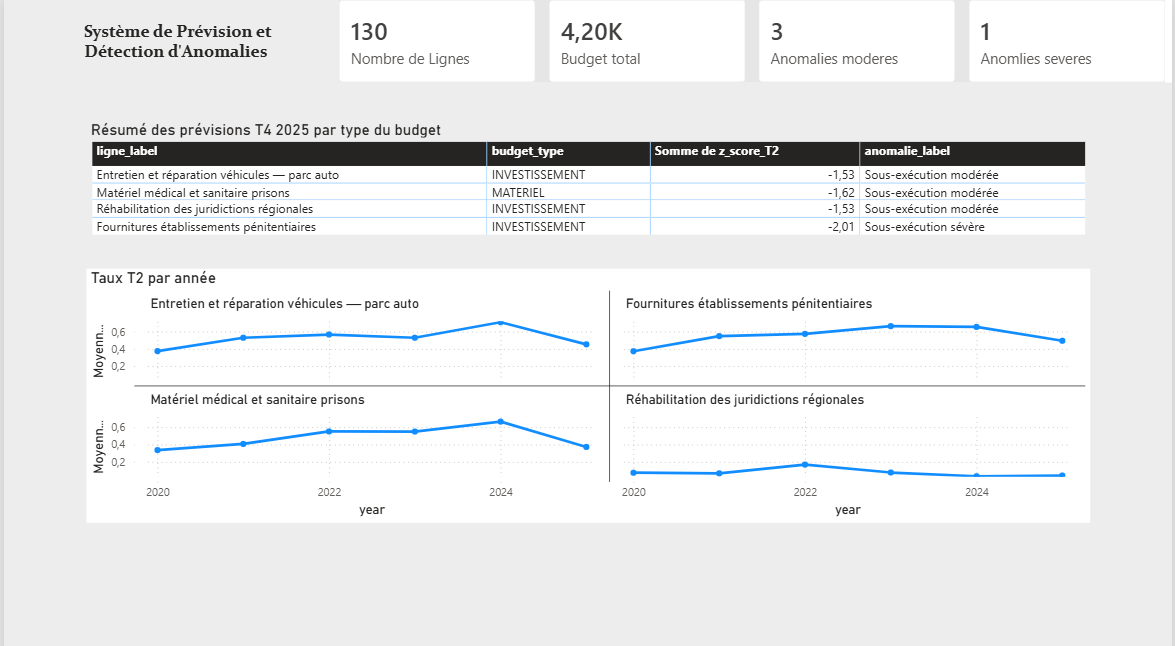
\includegraphics[width=0.98\textwidth]{figures/powerbidash_page2.png}
     \caption{\textbf{Page 2 du tableau de bord~: d\'etection d'anomalies et contexte historique.}
     La page recense les lignes signal\'ees par le module statistique (table centrale~: intitul\'e,
     cat\'egorie, z-score T2, label de s\'ev\'erit\'e) et les met en perspective via un panneau
     de \textit{small multiples} retra\c{c}ant l'\'evolution du taux T2 sur six exercices
     (2020--2025) pour chaque ligne anormale.}
     \label{fig:pbi_page2}
 \end{figure}

%================================================================
\phantomsection
\subsection*{5.4 \quad Apports op\'erationnels}
\addcontentsline{toc}{subsection}{5.4 Apports op\'erationnels et perspectives}
%================================================================

\subsubsection*{5.4.1 \quad Valeur ajout\'ee pour la DPPF}

Le système de pilotage apporte cinq avantages concrets~:

\begin{enumerate}
    \item \textbf{Alerte précoce ciblée.}

    Plutôt que de submerger les gestionnaires sous des dizaines d'indicateurs
    génériques, le système isole les quatre lignes anormales parmi 130, focalisant
    l'attention analytique sur les enjeux opérationnels réels et réduisant
    significativement le temps consacré aux investigations exploratoires.

    \item \textbf{Transparence des prévisions.}

    Les gestionnaires sont informés du fait que la prévision relative à
    l'\textsc{Investissement} présente une stabilité inférieure à celle de
    la catégorie \textsc{Personnel}, et calibrent en conséquence le degré de
    confiance accordé à chaque prédiction.

    \item \textbf{Interactivité et réduction du délai d'analyse.}

    En l'absence du tableau de bord, un responsable de programme devait commander
    un rapport manuel décrivant l'exécution ligne par ligne (un à deux jours de
    délai). Le filtrage interactif réduit cette opération à quelques dizaines
    de secondes, conférant ainsi au système une réactivité opérationnelle
    sans équivalent dans le dispositif antérieur.

    \item \textbf{Préparation simplifiée des audits et rapports trimestriels.}

    Les rapports d'exécution trimestriels, jusqu'ici produits manuellement,
    peuvent désormais être partiellement automatisés~: les exports Excel
    générés par le tableau de bord fournissent des données validées et
    directement exploitables.

    \item \textbf{Extensibilité et améliorations futures.}

    À mesure que des sources de données plus granulaires (notamment GID)
    deviendront accessibles, le système pourra être enrichi de manière
    incrémentale sans nécessiter de refonte architecturale~: seuls les
    modèles Python et les fichiers Excel intermédiaires évoluent.

\end{enumerate}

\subsubsection*{5.4.2 \quad Recommandations de déploiement et gouvernance}

L'approche reste celle adopt\'ee en Machine Learning appliqu\'e : le syst\`eme est un outil d'aide
à la décision, pas un remplaçant pour l'expertise métier. Chaque alerte doit déclencher une
investigation humaine et une validation par un responsable capable de contextualiser les
résultats, vérifier les données source, et prendre les décisions opérationnelles appropriées.


\newpage
\bibliography{references}

\end{document}